% !TeX spellcheck = en_US
% COMPILE WITH LuaLatex !!!

% Other paper formats are possible: aspectratio = 43 (4:3), 169 (16:9), etc...
% If you set the option "handout", overlay effects will be ignored:
%\documentclass[aspectratio=43,handout]{beamer}
\documentclass[8pt, t,
% aspectratio=169,% for widescreen (16:9) presentations
aspectratio=43,% for traditional (4:3) presentations
%handout,%
]{beamer}

\usepackage[utf8]{}
\usepackage[T1]{fontenc}
\usepackage{circledsteps}

% Title and author
\title{Ecohydraulic Engineering\\ of Water Resources\\{\tiny Analysis \& Management of Connectivity}} % If needed, manually add line breaks with "\\"
\author[Dr. sc. (PhD) Sebastian Schwindt]{Dr. sc. (PhD) Sebastian Schwindt}
%\title{\footnotesize If the title is very long and does not fit easily, you might want to manually use a smaller font here.}

\subtitle{}

\usetheme{lww}

% for ecosystem services mitigating extreme weather, see https://en.wikipedia.org/wiki/Millennium_Ecosystem_Assessment
\begin{document}

% Create the titlepage
\maketitle

% Optional: show the outline
%\begin{frame}{Table of Contents}
%	\tableofcontents
%\end{frame}

%%%%%%%%%%%%%%%%%%%%%%%%%%%%%%%%%%% slides %%%%%%%%%%%%%%%%%%%%%%%%%%%%%%%%%%%%%
\section*{Connectivity Dimensions}

\begin{frame}{\secname}
	\begin{tikzpicture}
		\clip (0,0) rectangle (\paperwidth,\paperheight);
		\onslide<1->{
			\begin{scope}
				\node[anchor=south west, xshift=0.08\paperwidth, yshift=0.14\paperheight] {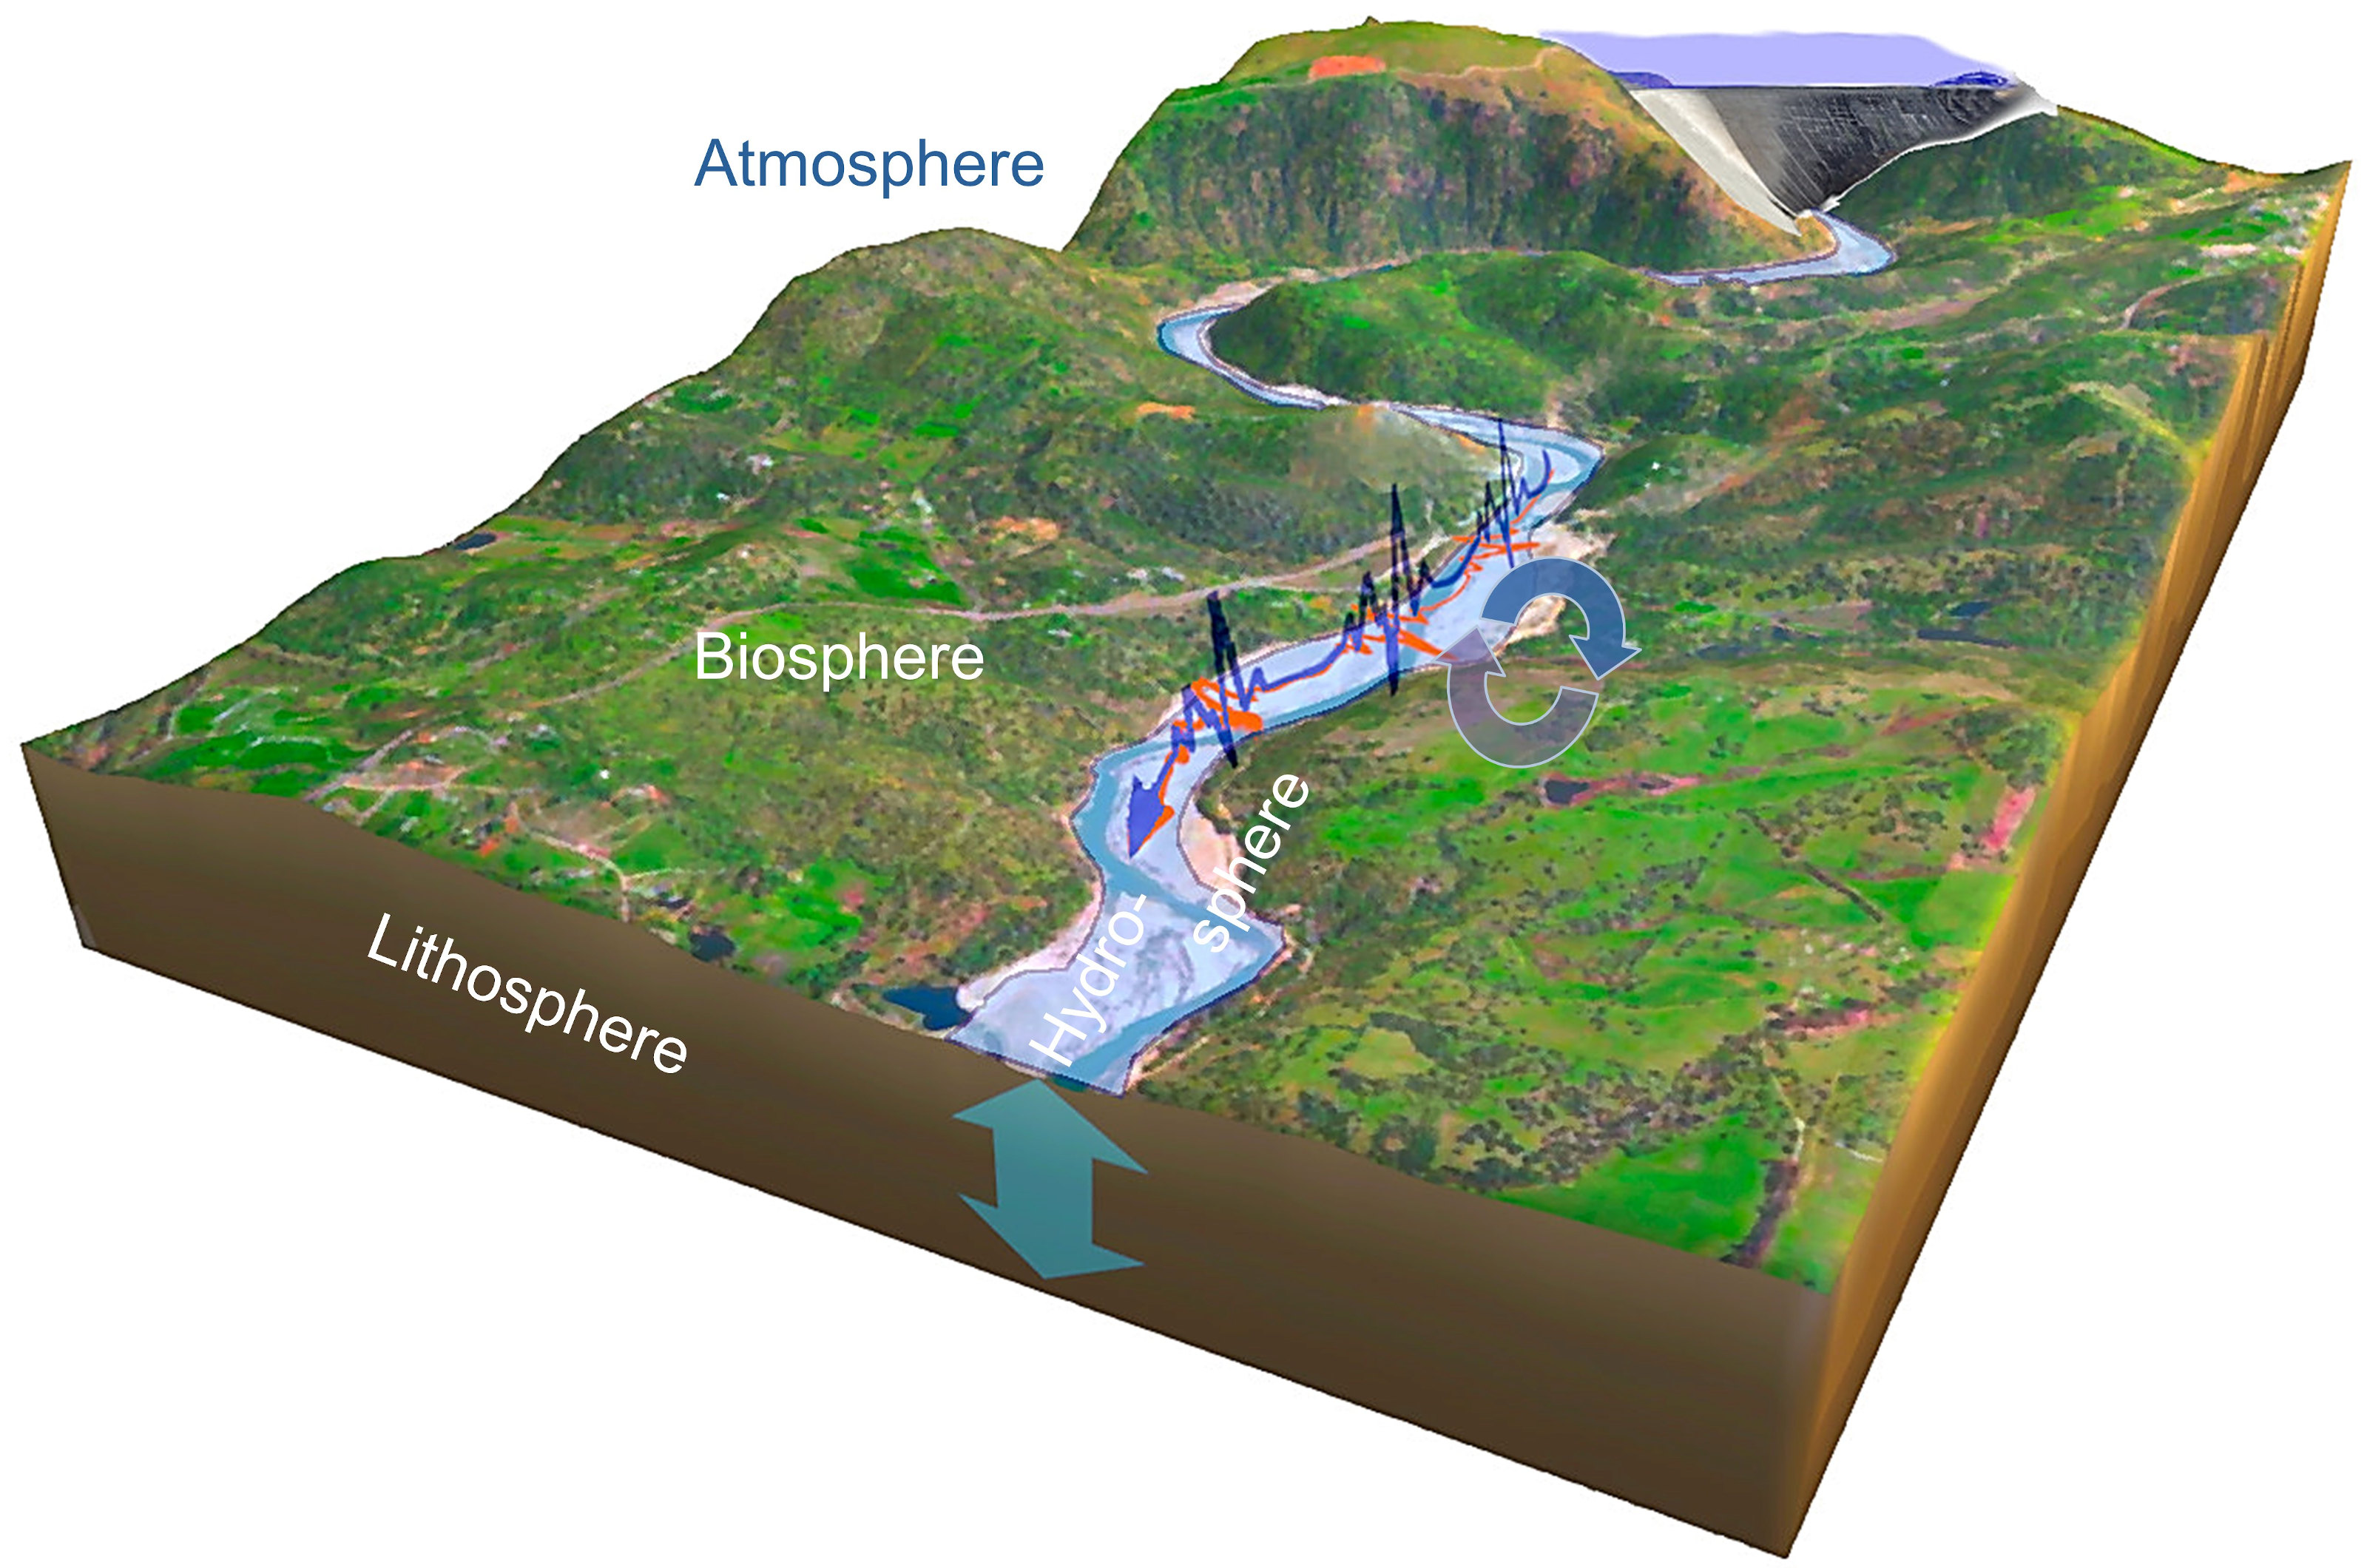
\includegraphics[width=0.82\paperwidth]{hyconnect-with-dam}};
		\end{scope}}
		\onslide<1->{
			\fill[unisblue,opacity=0.7,xshift=-0.91\paperwidth,yshift=0.86] (\paperwidth,0.86\paperheight) circle (0.11\paperheight);
			% place text in circle
			\node at (\paperwidth,0.865\paperheight)[xshift=-0.908\paperwidth,yshift=0.865,text width=0.135\paperwidth,align=center]{\bf \large {\textcolor{white}{Spatio-temporal axes}}};
		}
	\end{tikzpicture}
\end{frame}

\subsection{Space \& Time Axes}
\begin{frame}{\secname: \subsecname}
	\begin{tikzpicture}
		\clip (0,0) rectangle (\paperwidth,\paperheight);
		\onslide<1-1>{
			\begin{scope}
				\node[anchor=south west, xshift=0.\paperwidth, yshift=0.2\paperheight] {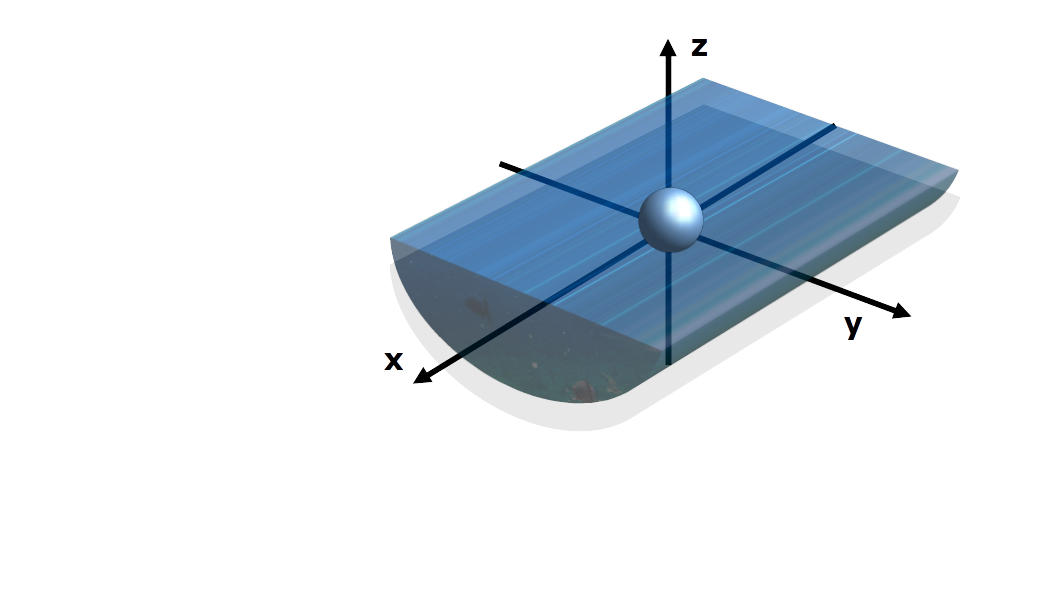
\includegraphics[width=0.9\paperwidth]{connectivity-dimensions-0}};
		\end{scope}}
		\onslide<2->{
			\begin{scope}
				\node[anchor=south west, xshift=0.\paperwidth, yshift=0.2\paperheight] {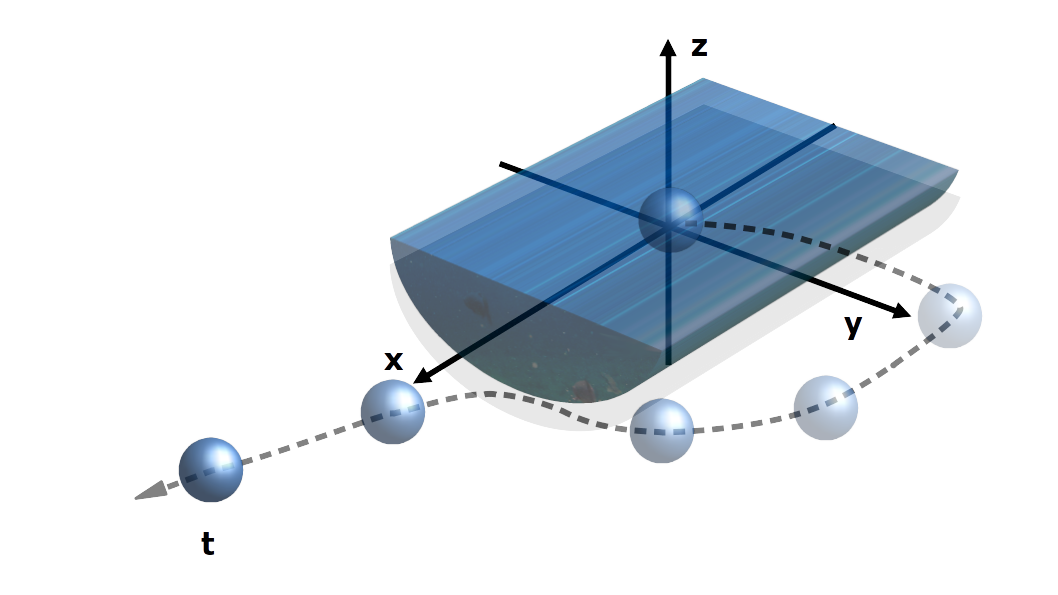
\includegraphics[width=0.9\paperwidth]{connectivity-dimensions-1}};
		\end{scope}}
	\end{tikzpicture}
\end{frame}

\section*{Engineering}
\subsection{Problem \& Solution}
\begin{frame}{\secname: \subsecname}
	\begin{tikzpicture}
		\clip (0,0) rectangle (\paperwidth,\paperheight);
		\onslide<1->{
			\begin{scope}
				\node[anchor=south west, xshift=0.\paperwidth, yshift=0.235\paperheight] {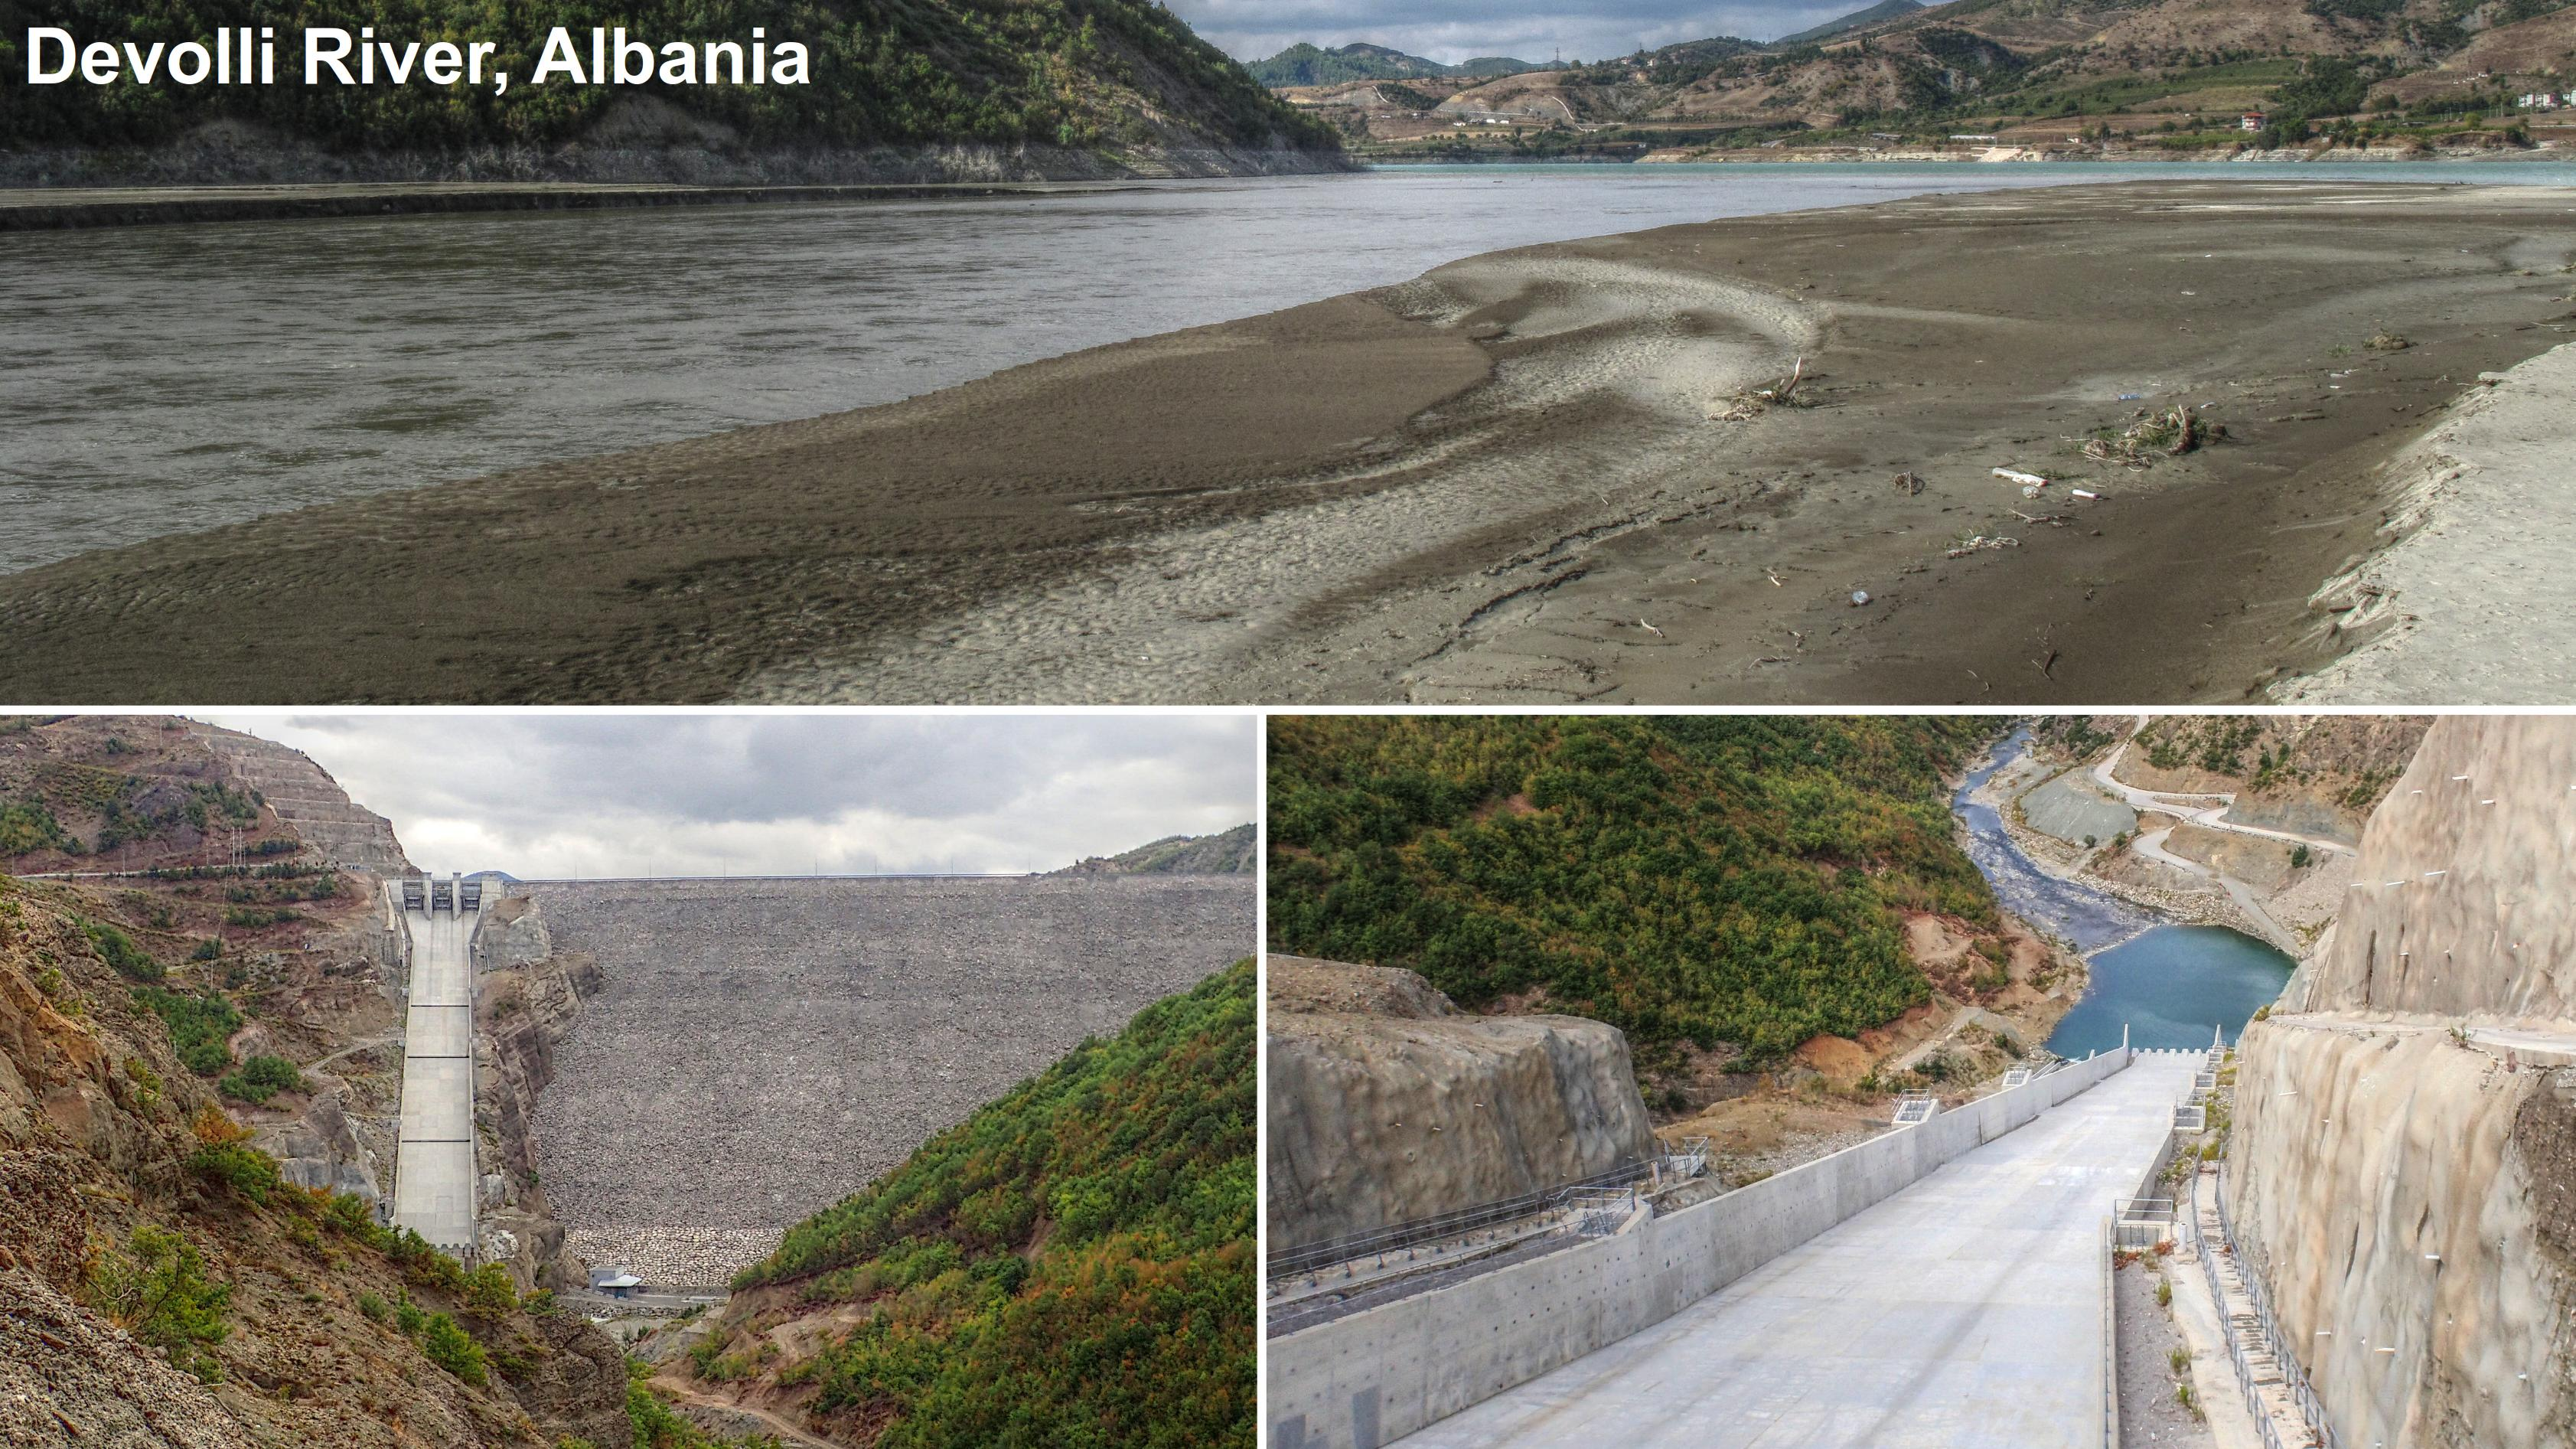
\includegraphics[width=0.88\paperwidth]{engineering-image-assembley}};
		\end{scope}}
		\onslide<2->{
		\begin{scope}
				\node[anchor=south west, xshift=0.03\paperwidth, yshift=0.235\paperheight] {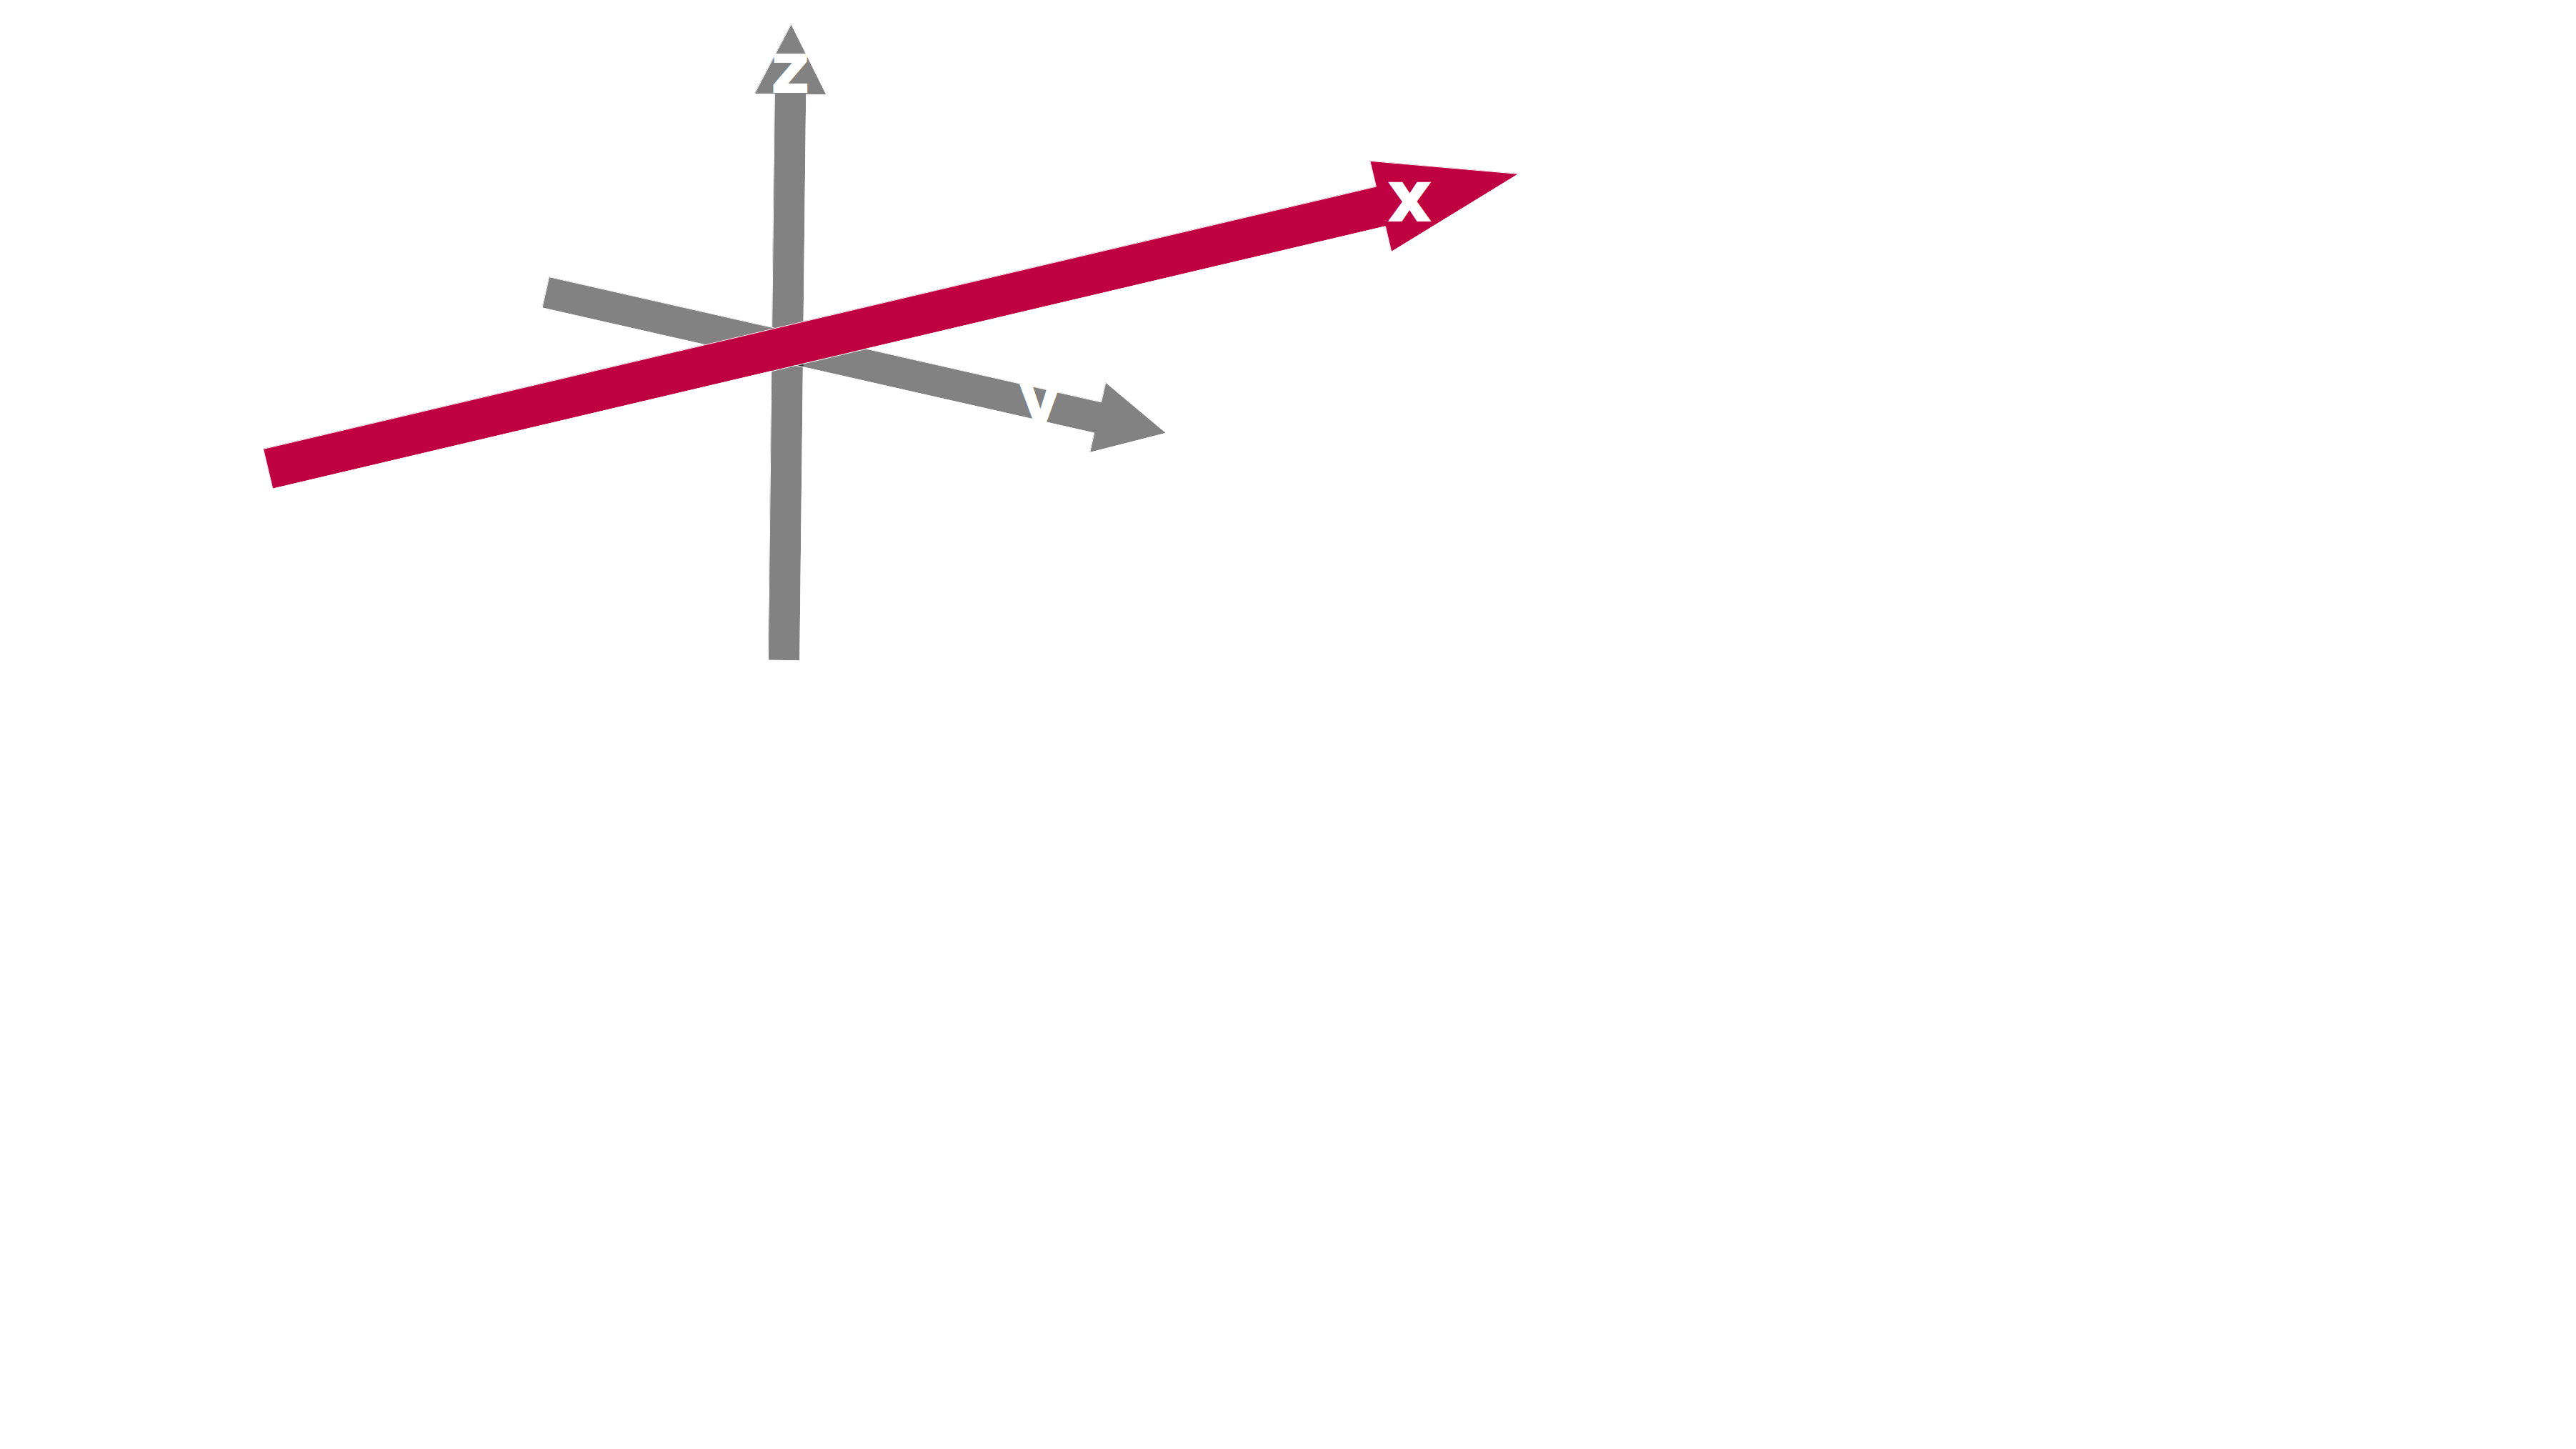
\includegraphics[width=0.88\paperwidth]{engineering-image-assembley-arrows}};
		\end{scope}}
	\end{tikzpicture}
\end{frame}


%\begin{frame}{\secname: \subsecname}
%	\begin{tikzpicture}
%		\clip (0,0) rectangle (\paperwidth,\paperheight);
%		\onslide<1->{
%			\begin{scope}
%				\node[anchor=south west, xshift=0.\paperwidth, yshift=0.235\paperheight] {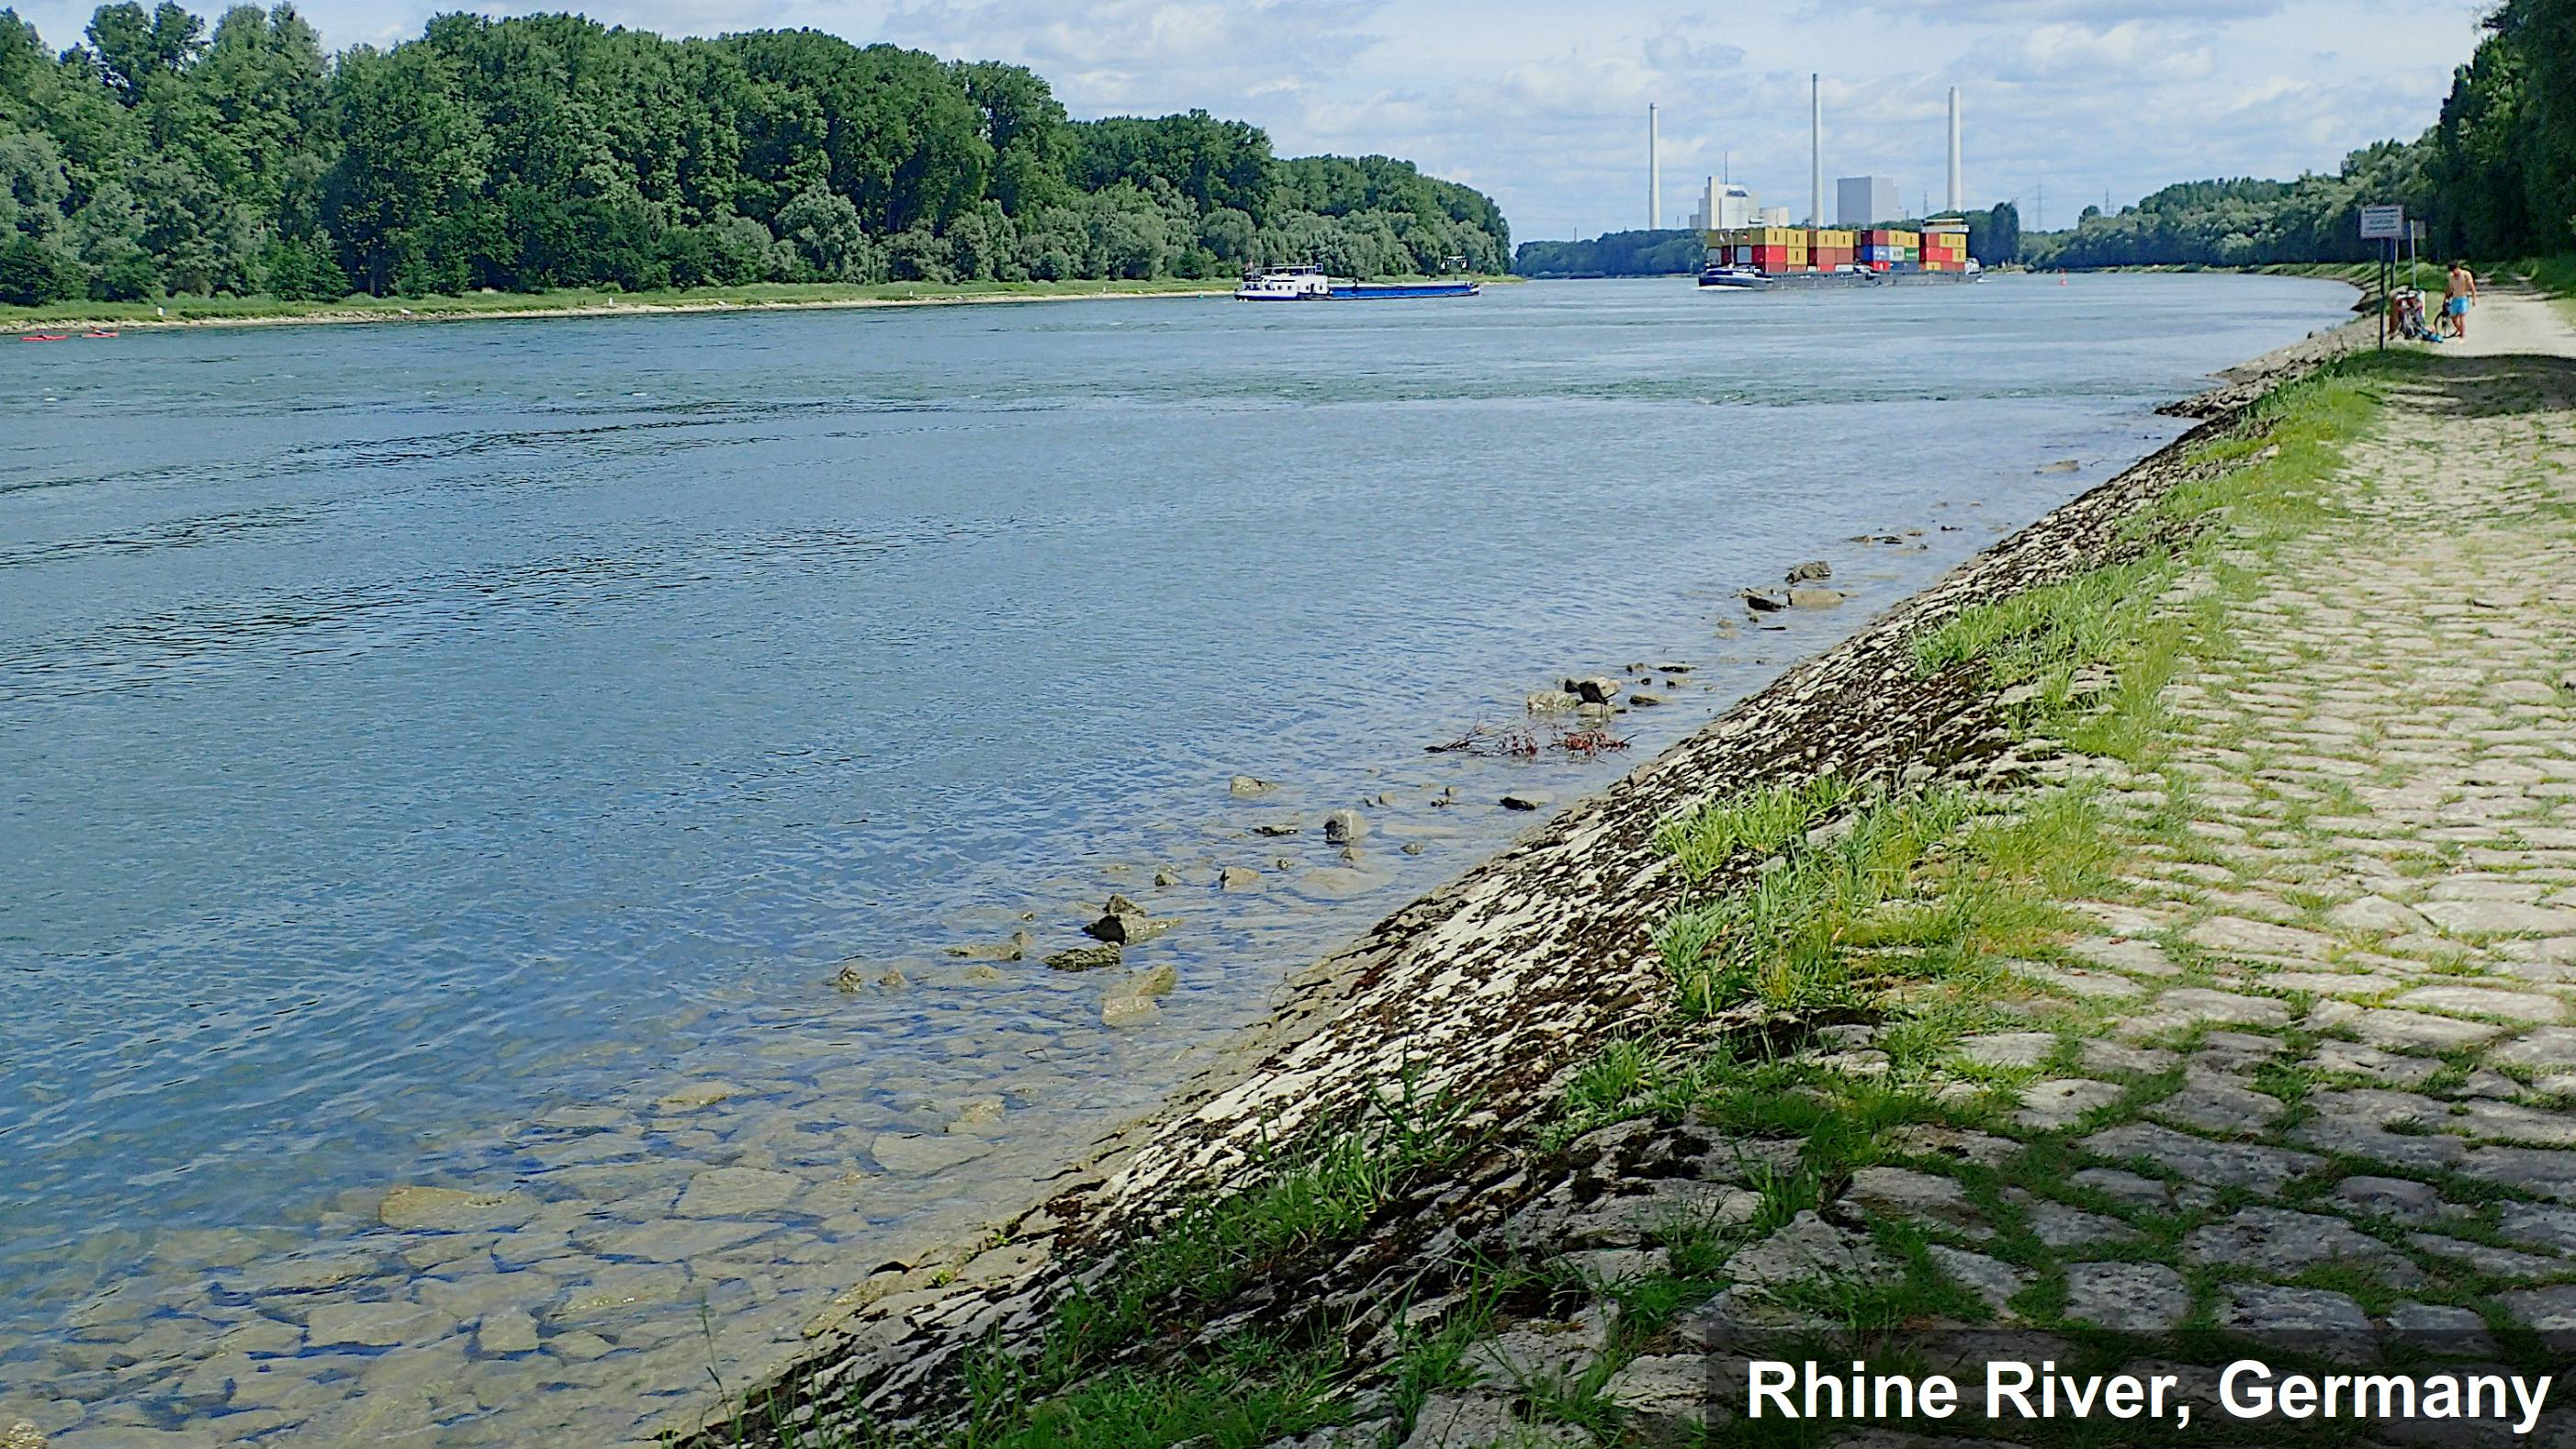
\includegraphics[width=0.88\paperwidth]{rhine-ww}};
%		\end{scope}}
%		\onslide<2->{
%			\begin{scope}
%				\node[anchor=south west, xshift=0.\paperwidth, yshift=0.235\paperheight] {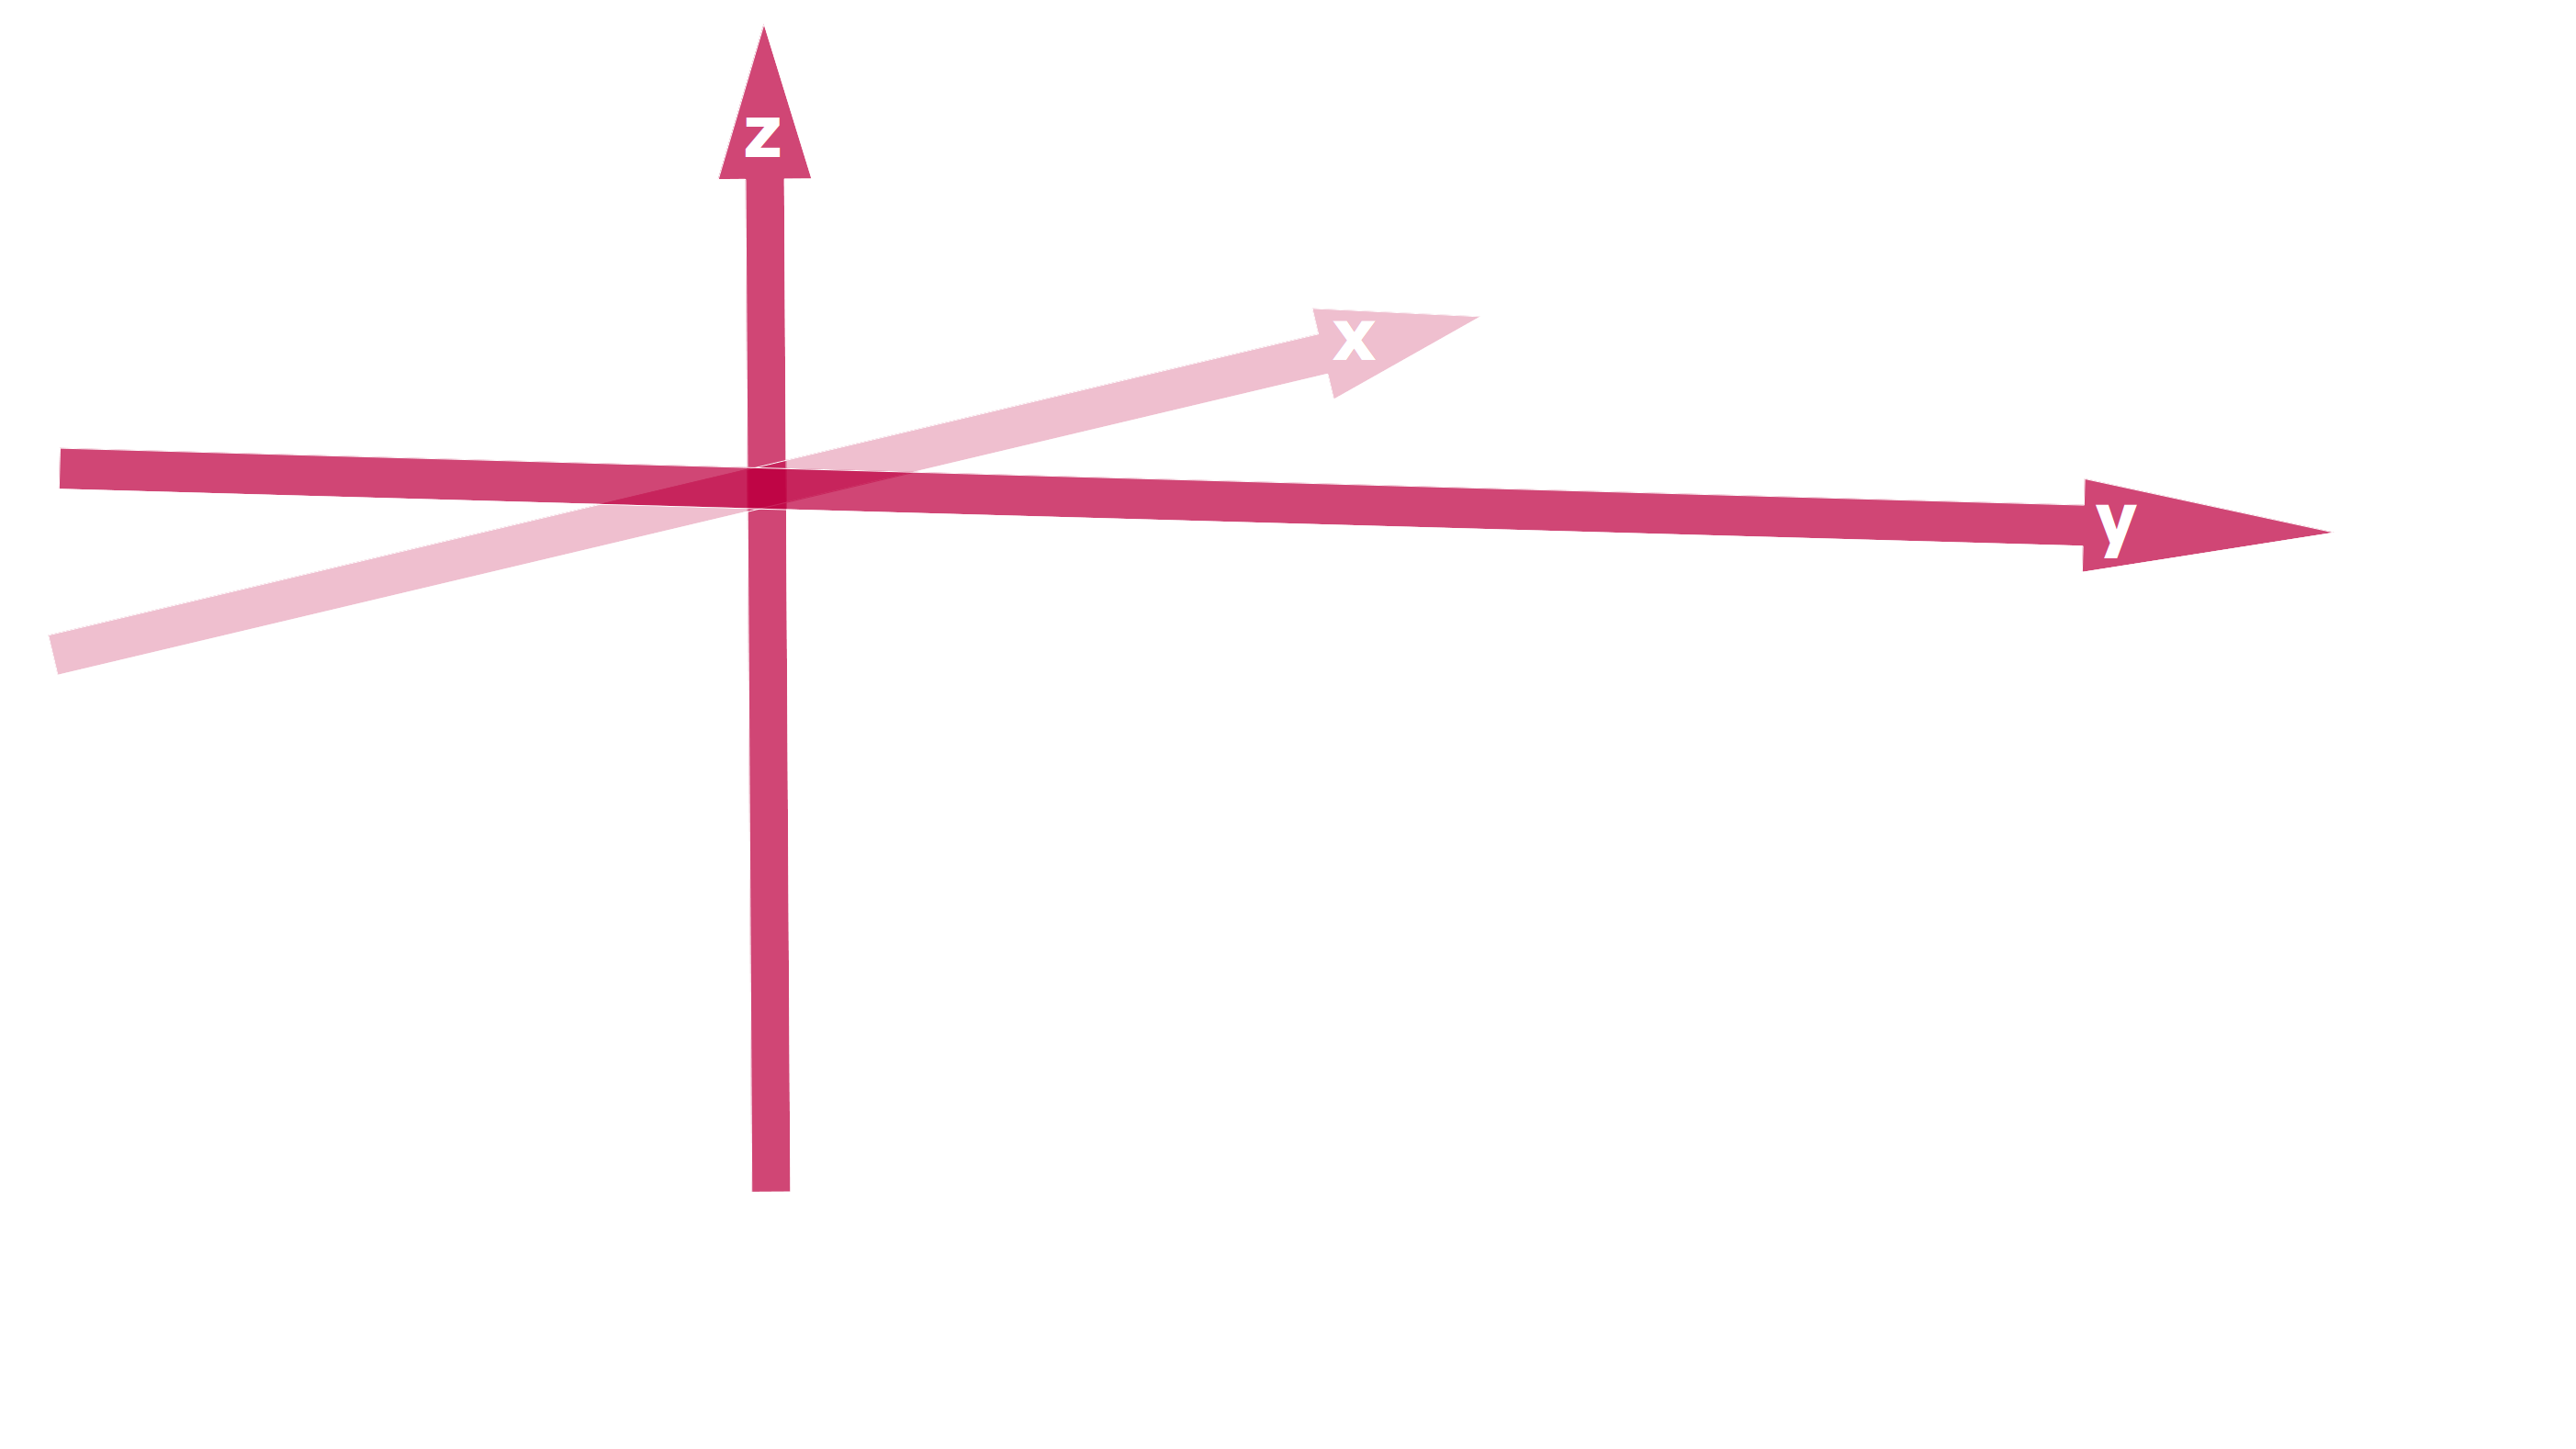
\includegraphics[width=0.88\paperwidth]{rhine-ww-arrows}};
%		\end{scope}}
%	\end{tikzpicture}
%\end{frame}




\begin{frame}{\secname: \subsecname}
	Reconnecting the x-axis: harm vs. utility of dams
	\begin{tikzpicture}
		\clip (0,0) rectangle (\paperwidth,\paperheight);
		\onslide<1->{
		\begin{scope}
				\node[anchor=south west, xshift=0.\paperwidth, yshift=0.235\paperheight] {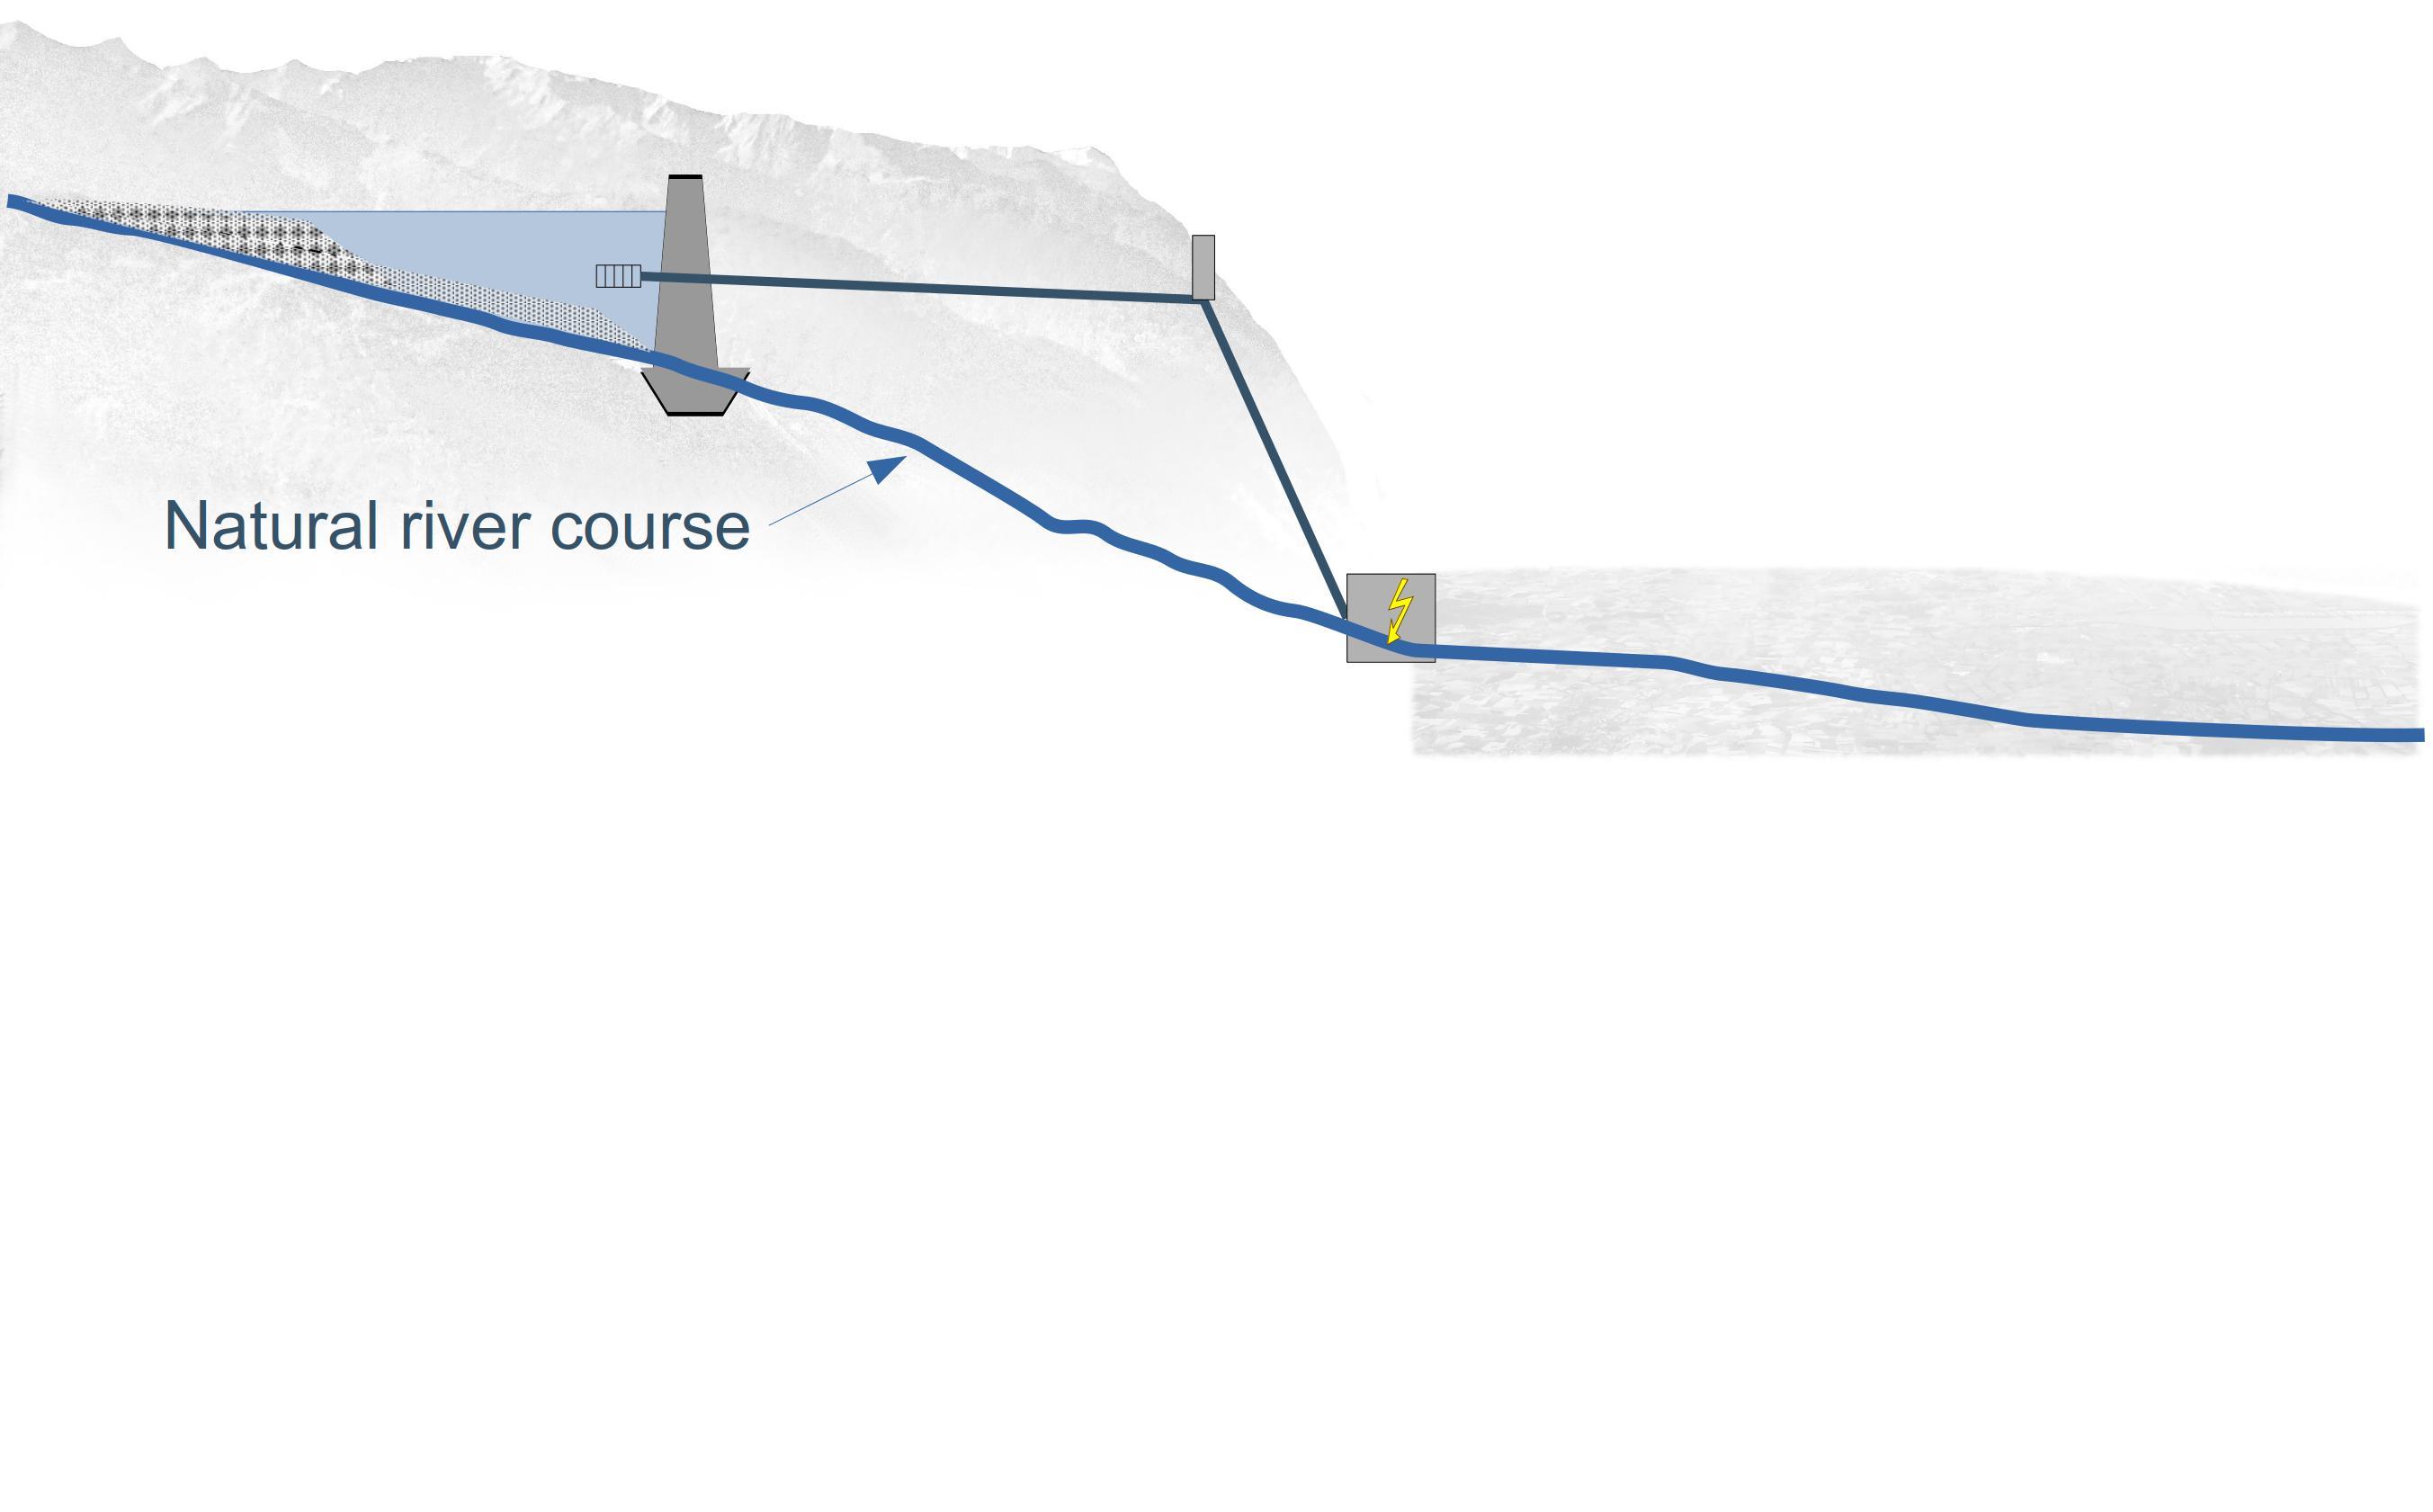
\includegraphics[width=0.88\paperwidth]{dam-scheme-0}};
		\end{scope}}
		\onslide<2->{
			\begin{scope}
				\node[anchor=south west, xshift=0.\paperwidth, yshift=0.235\paperheight] {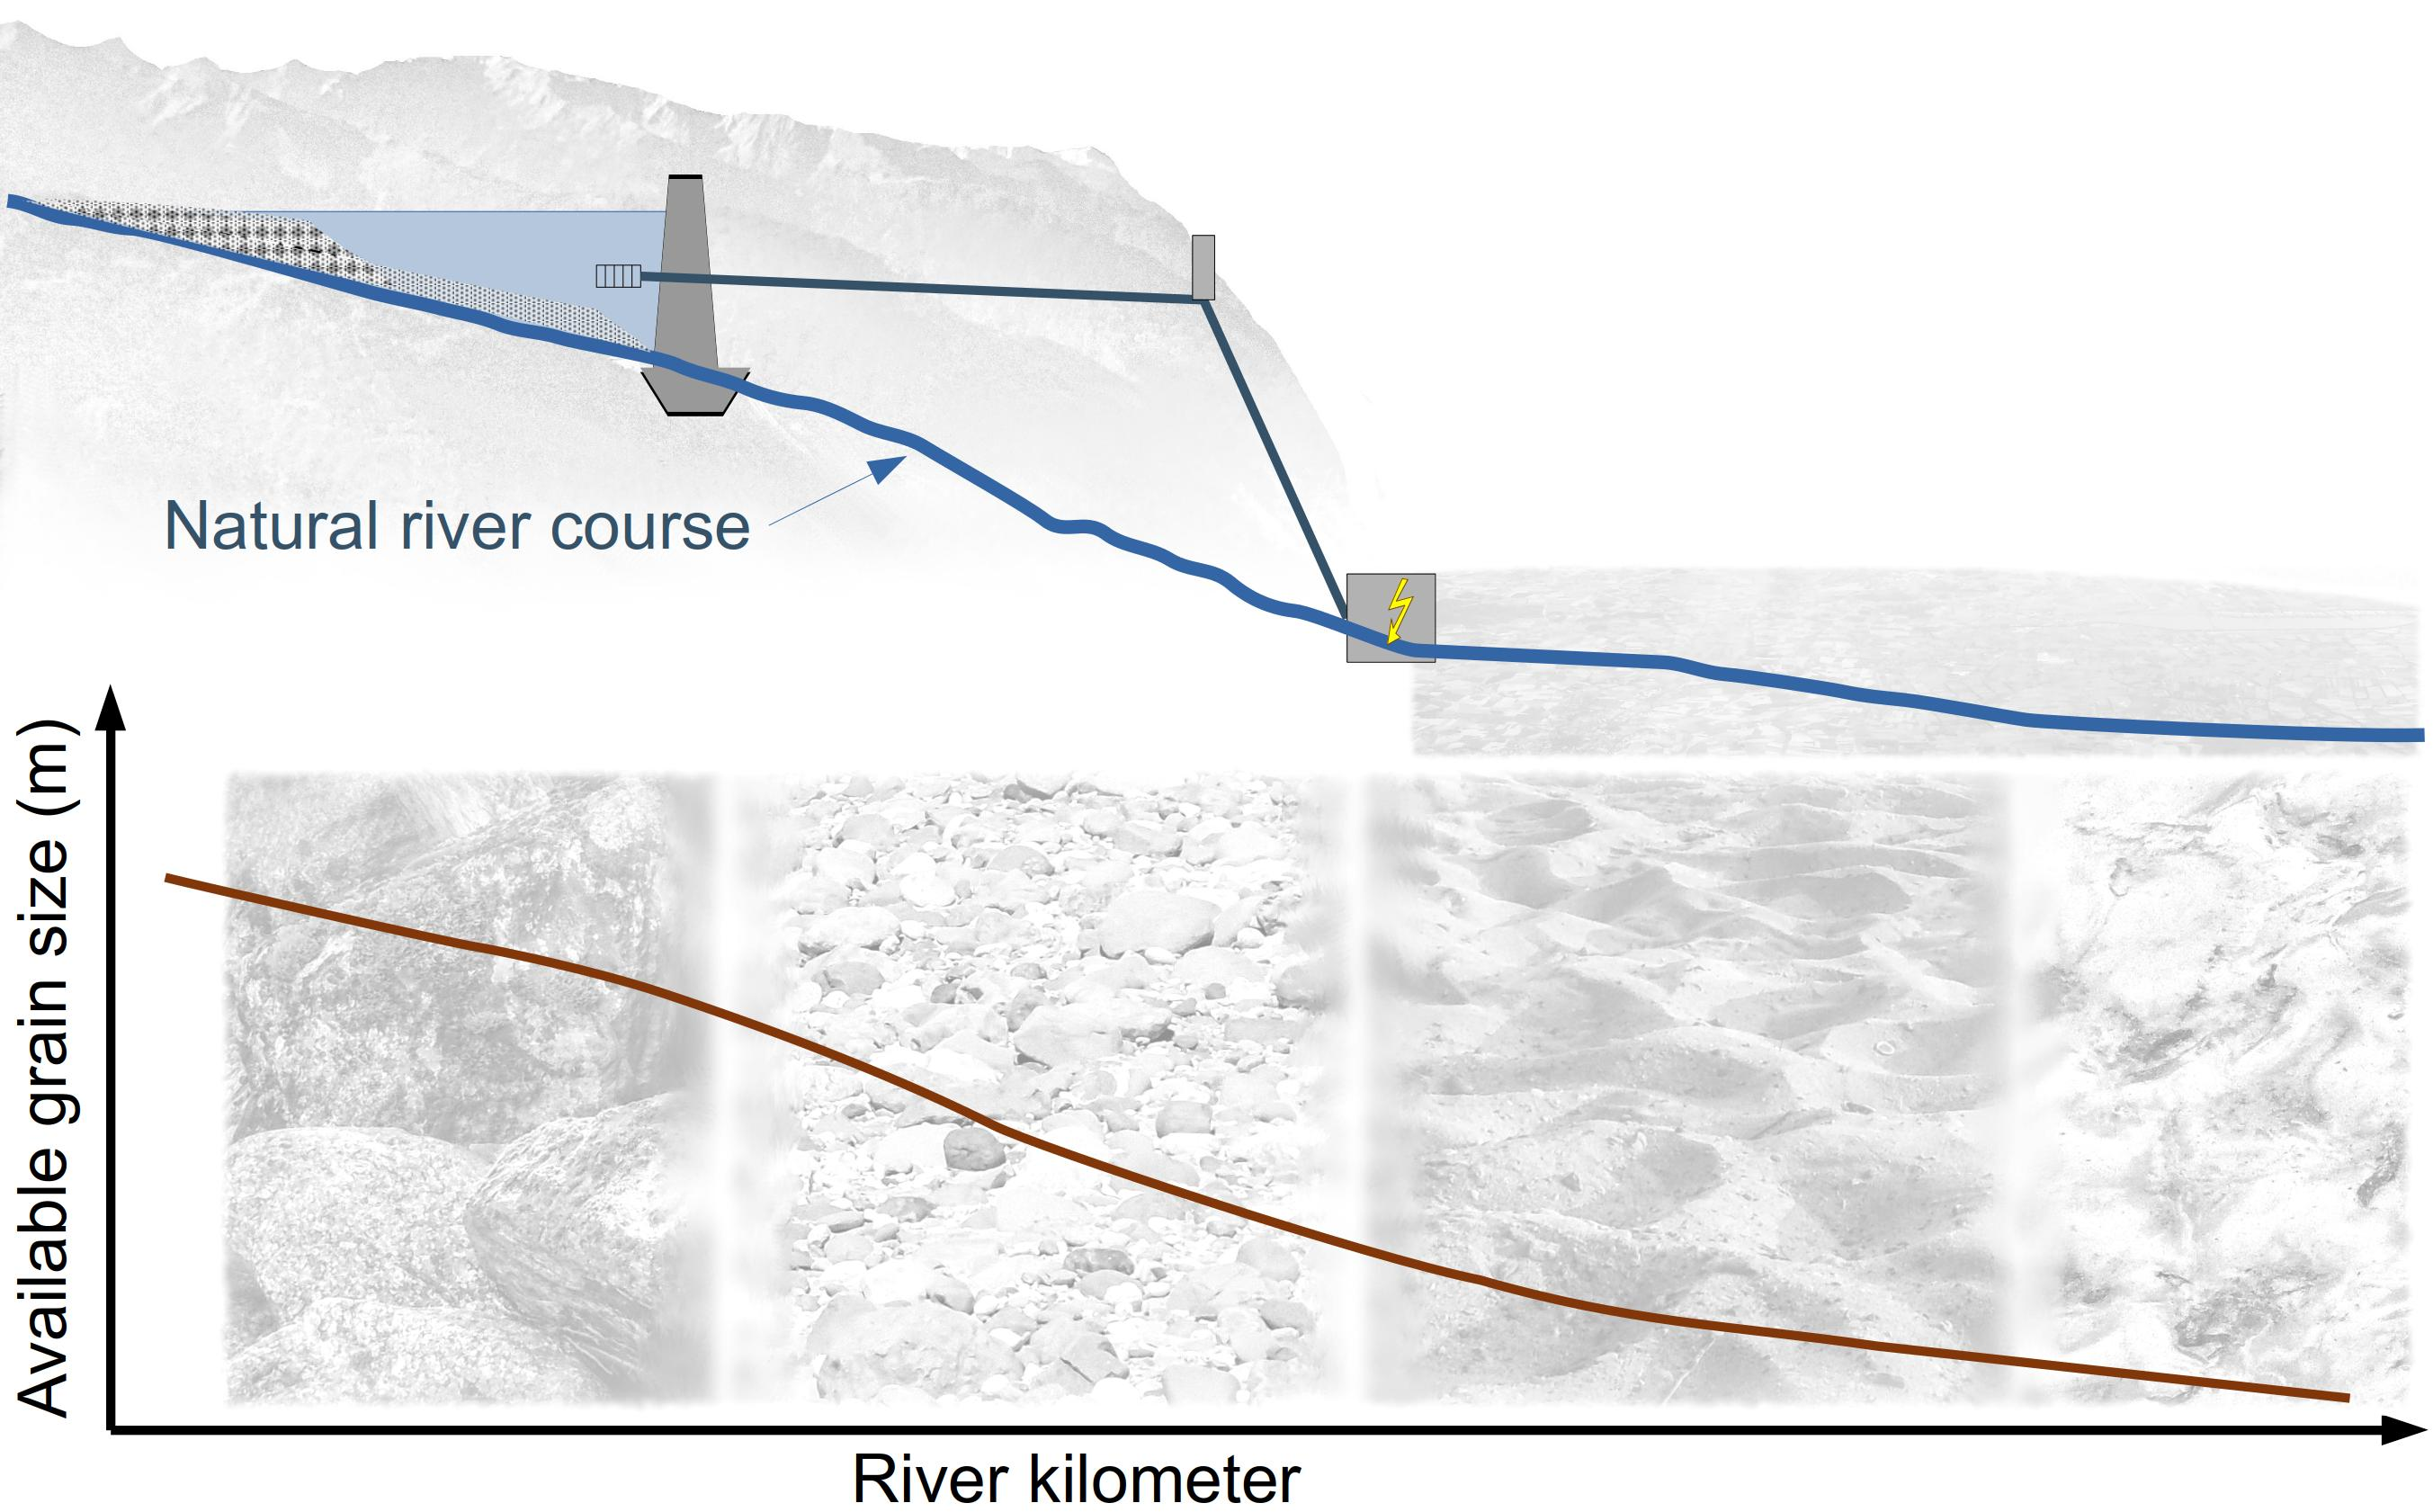
\includegraphics[width=0.88\paperwidth]{dam-scheme-1}};
		\end{scope}}
	\end{tikzpicture}
\end{frame}

%\begin{frame}{\secname: \subsecname}
%	\begin{tikzpicture}
%		\clip (0,0) rectangle (\paperwidth,\paperheight);
%		\onslide<1->{
%		\begin{scope}
%				\node[anchor=south west, xshift=0.\paperwidth, yshift=0.235\paperheight] {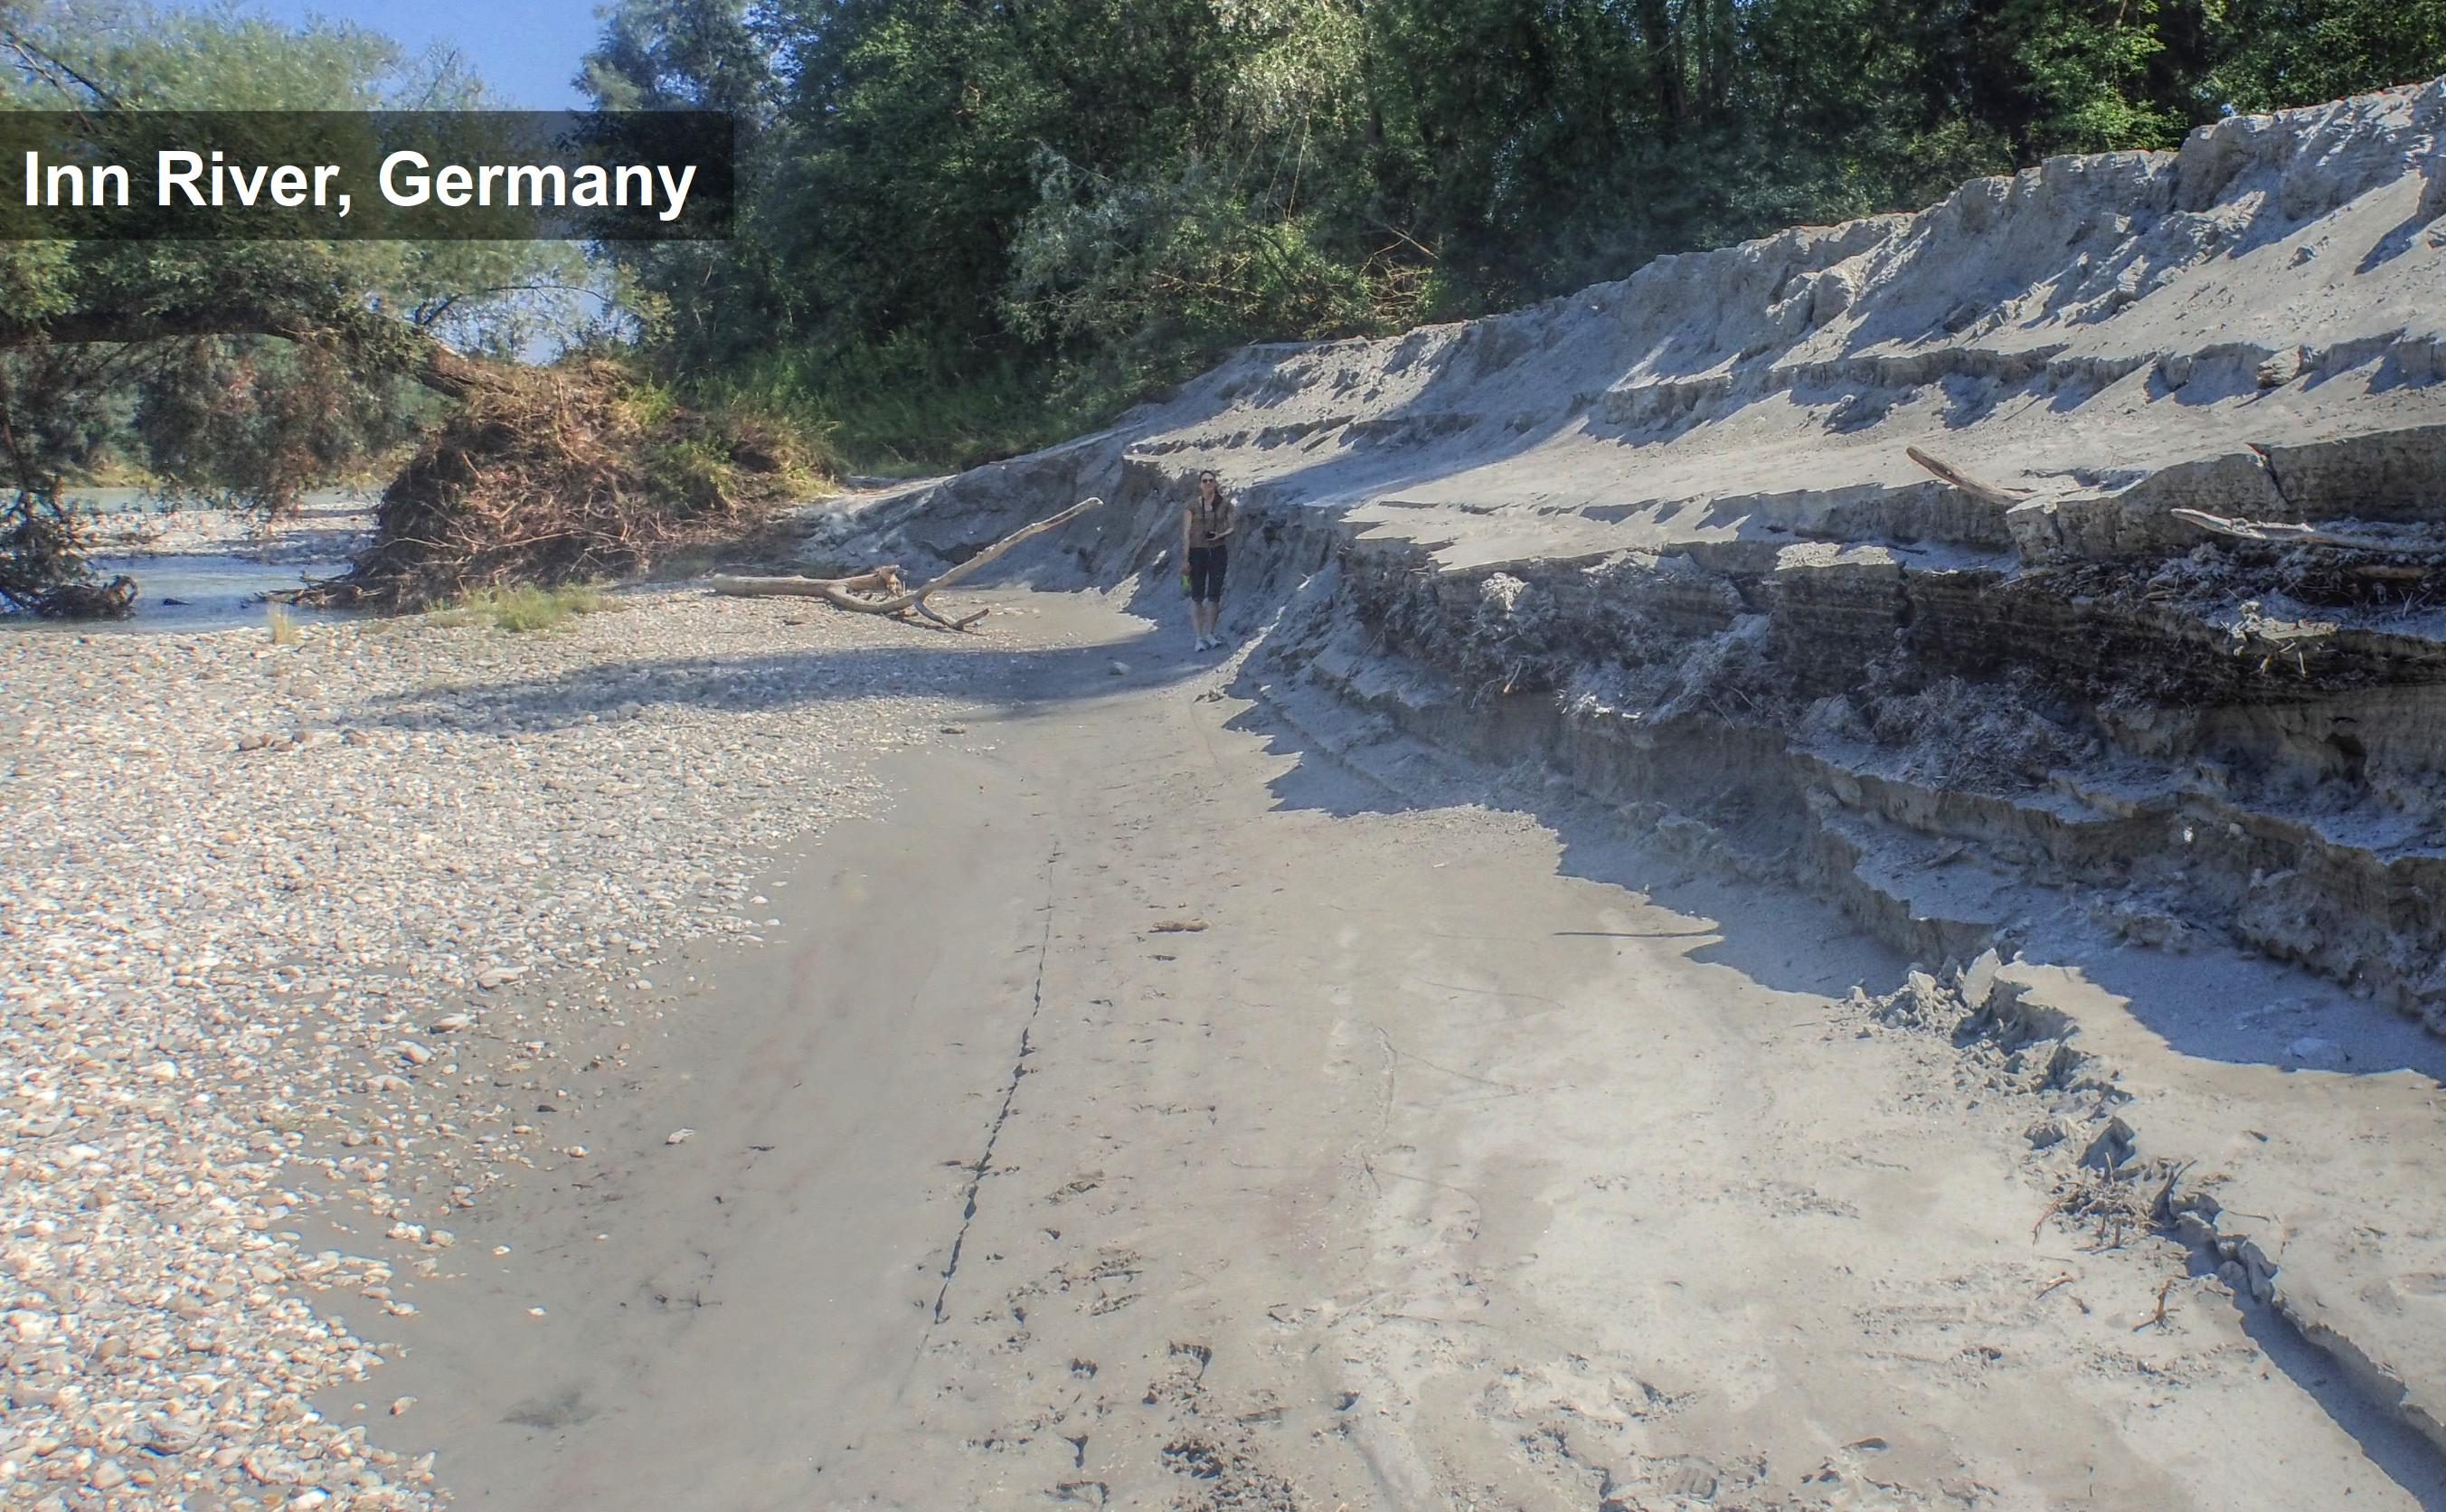
\includegraphics[width=0.88\paperwidth]{inn-sand-bank-ann}};
%		\end{scope}}
%	\end{tikzpicture}
%\end{frame}


{
\usebackgroundtemplate{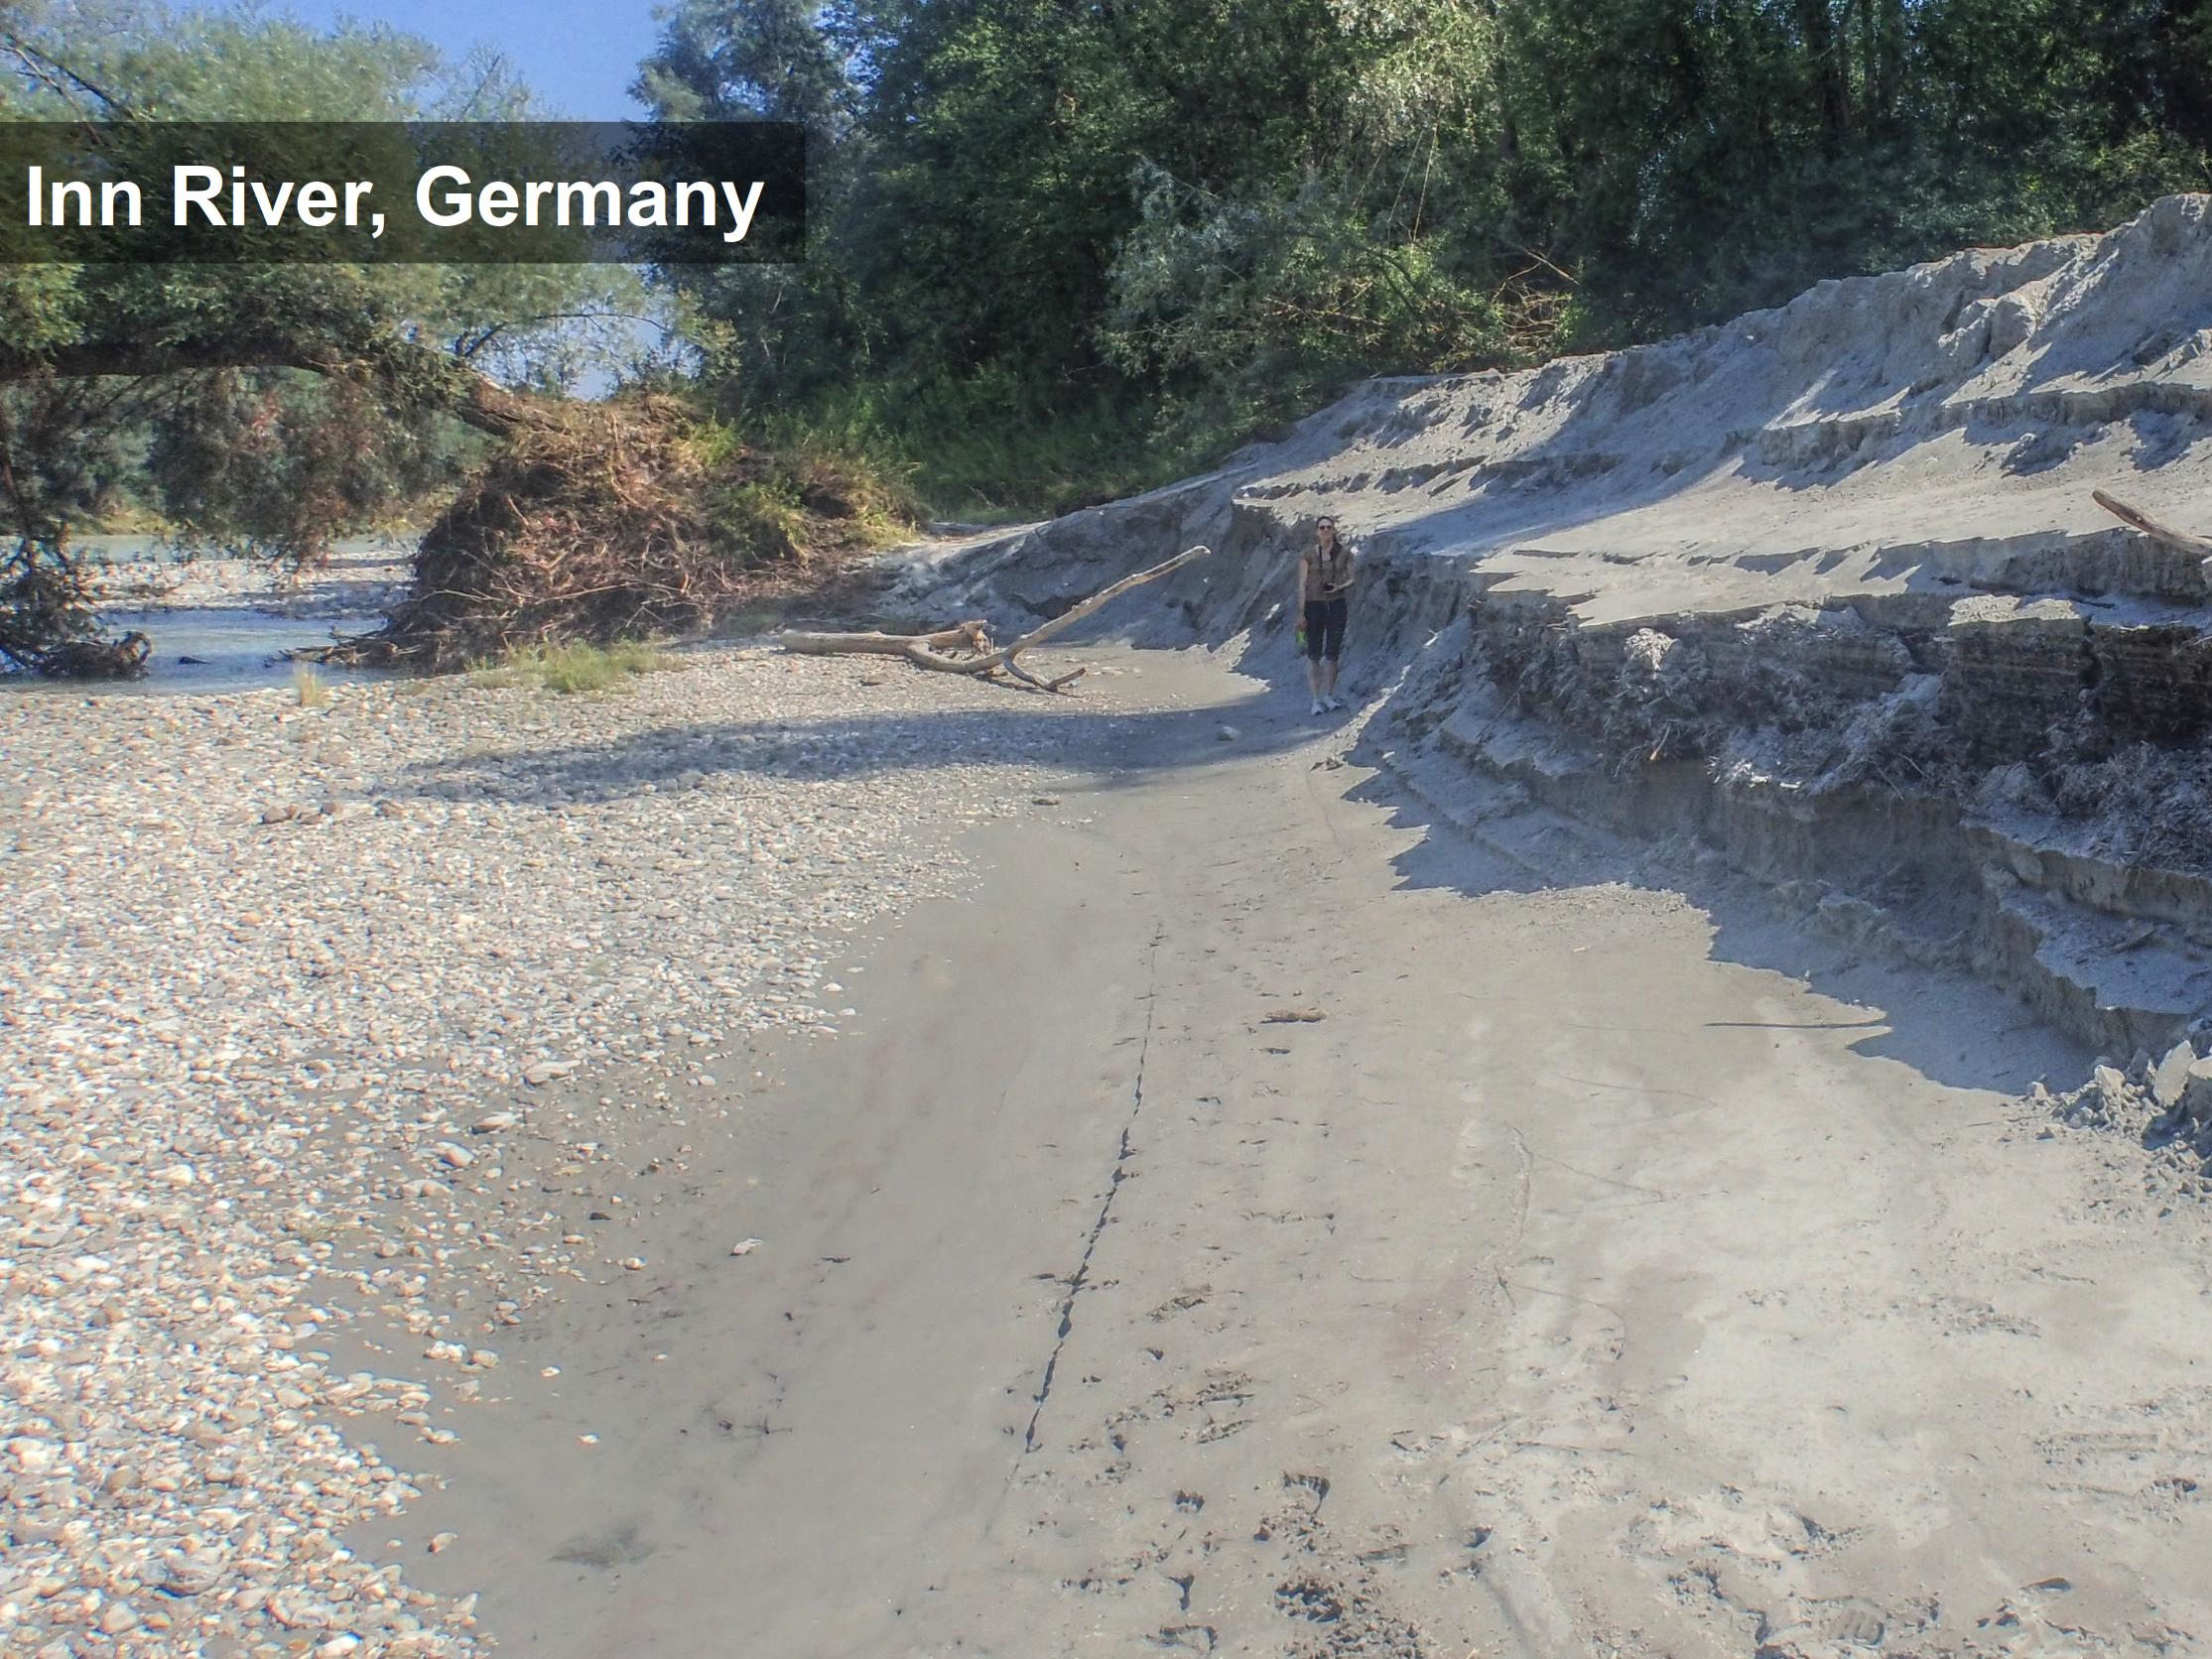
\includegraphics[width=\paperwidth]{inn-sand-bank-ann43.jpg}}%
\begin{frame}[plain]{}{\secname}
	\vspace{3cm}
	\onslide<2->{
	\begin{tcolorbox}[colbacktitle=hellblau!80!black, colback=hellblau!15!white, fonttitle=\bfseries, standard jigsaw,colframe=blue_light, bottom=0mm, middle=0mm, boxsep=0.2mm, opacityframe=0.5, opacityfill=0.75, opacitybacktitle=0.95, title filled, title={Challenges \& Opportunities}, size=fbox]
		\vspace{0.25cm}		 
		\begin{itemize}
			\item[\faChainBroken]\ \textbf{Dams disconnect river ecosystems}
			\item[\faChainBroken]\ No general solution available $\rightarrow$ Local actions\vspace{0.5cm}
			\item[\faChevronCircleRight]\ Optimize actions with fluvial sediment transport assessments
			\item[\faChevronCircleRight]\ Methods: Lab, field, and computer simulations\\			
			$\rightarrow$ Modeling sediment transport is complex: high uncertainty
		\end{itemize}
		\vspace{0.25cm}
	\end{tcolorbox}\smallskip}
\end{frame}}

\section{Longitudinal Connectivity {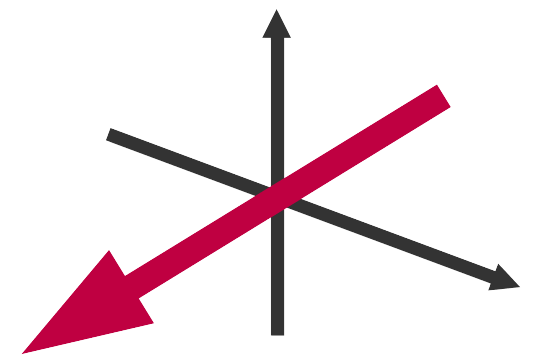
\includegraphics[height=15pt]{connectivity-x-small}}}

\subsection{Reservoir Sedimentation - Principles}


\subsection{Mountain River Engineering}
\begin{frame}{\secname\vspace{0.1cm}\\\textcolor{anthrazit!80!white}{\subsecname}}
	\begin{tikzpicture}
		\clip (0,0) rectangle (\paperwidth,\paperheight);
		\onslide<1->{
		\begin{scope}
				\node[anchor=south west, xshift=0.0\paperwidth, yshift=0.31\paperheight] {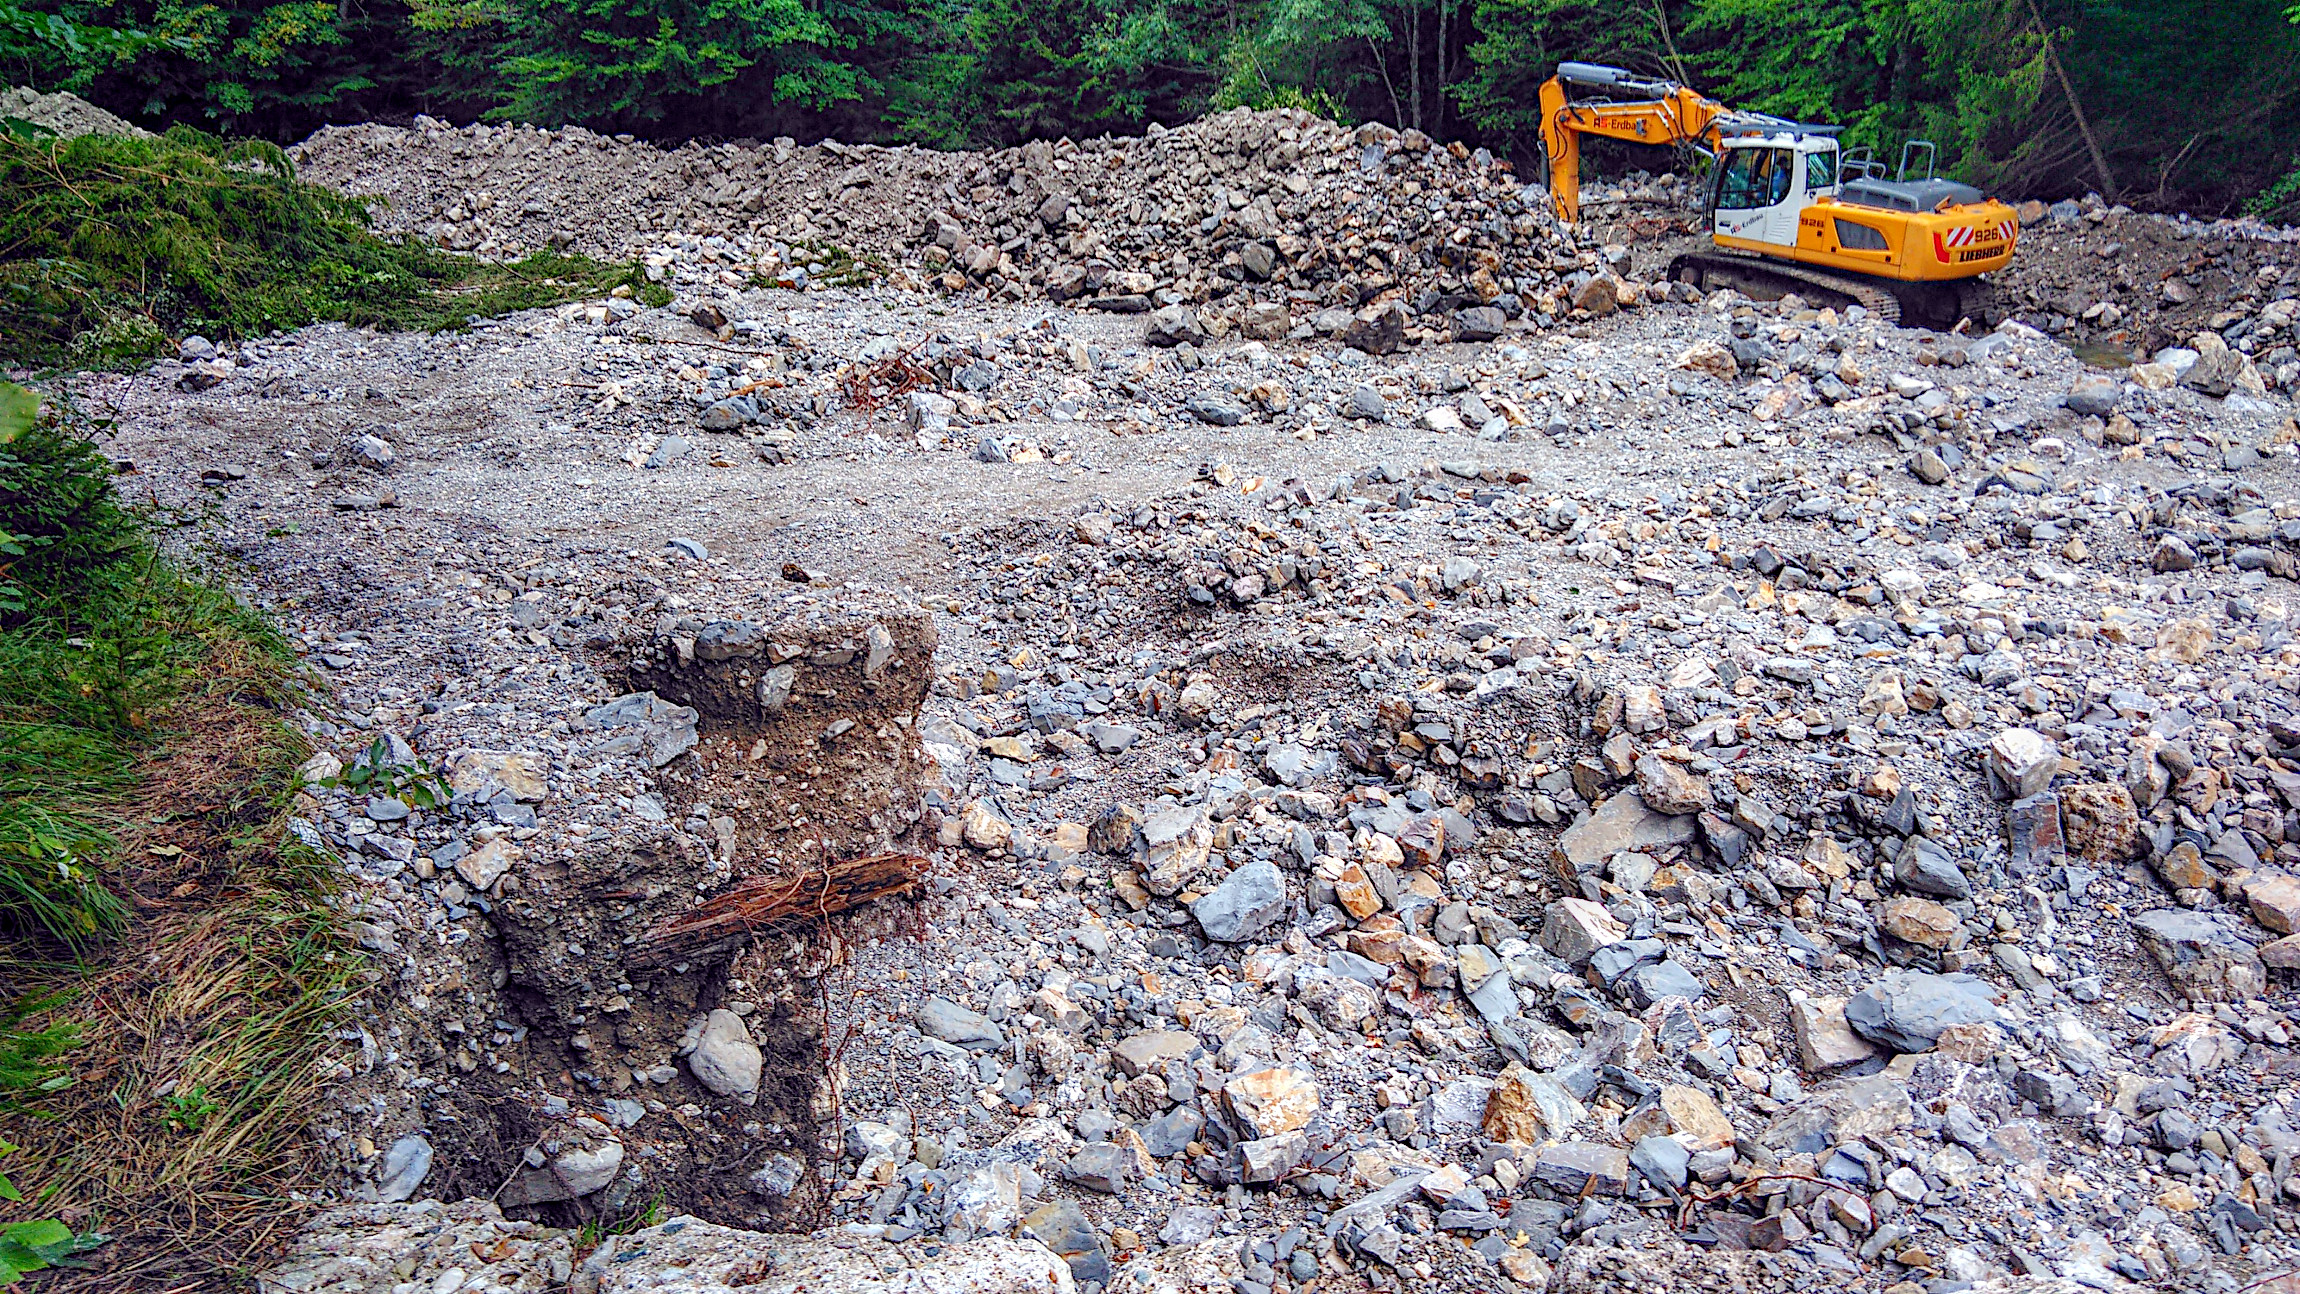
\includegraphics[width=0.865\paperwidth]{jenbach-bagger}};
		\end{scope}}
		\node[anchor=south west, xshift=0.33\paperwidth, yshift=2.13cm, text=black, text width=0.5\paperwidth,align=left]{\tiny \textcolor{gray}{Jenbach, Bavarian Alps}};
	\end{tikzpicture}
\end{frame}
\begin{frame}{\secname\vspace{0.1cm}\\\textcolor{anthrazit!80!white}{\subsecname}}
	\begin{tikzpicture}
		\clip (0,0) rectangle (\paperwidth,\paperheight);
		\onslide<1->{
			\begin{scope}
				\node[anchor=south west, xshift=0.0\paperwidth, yshift=0.31\paperheight] {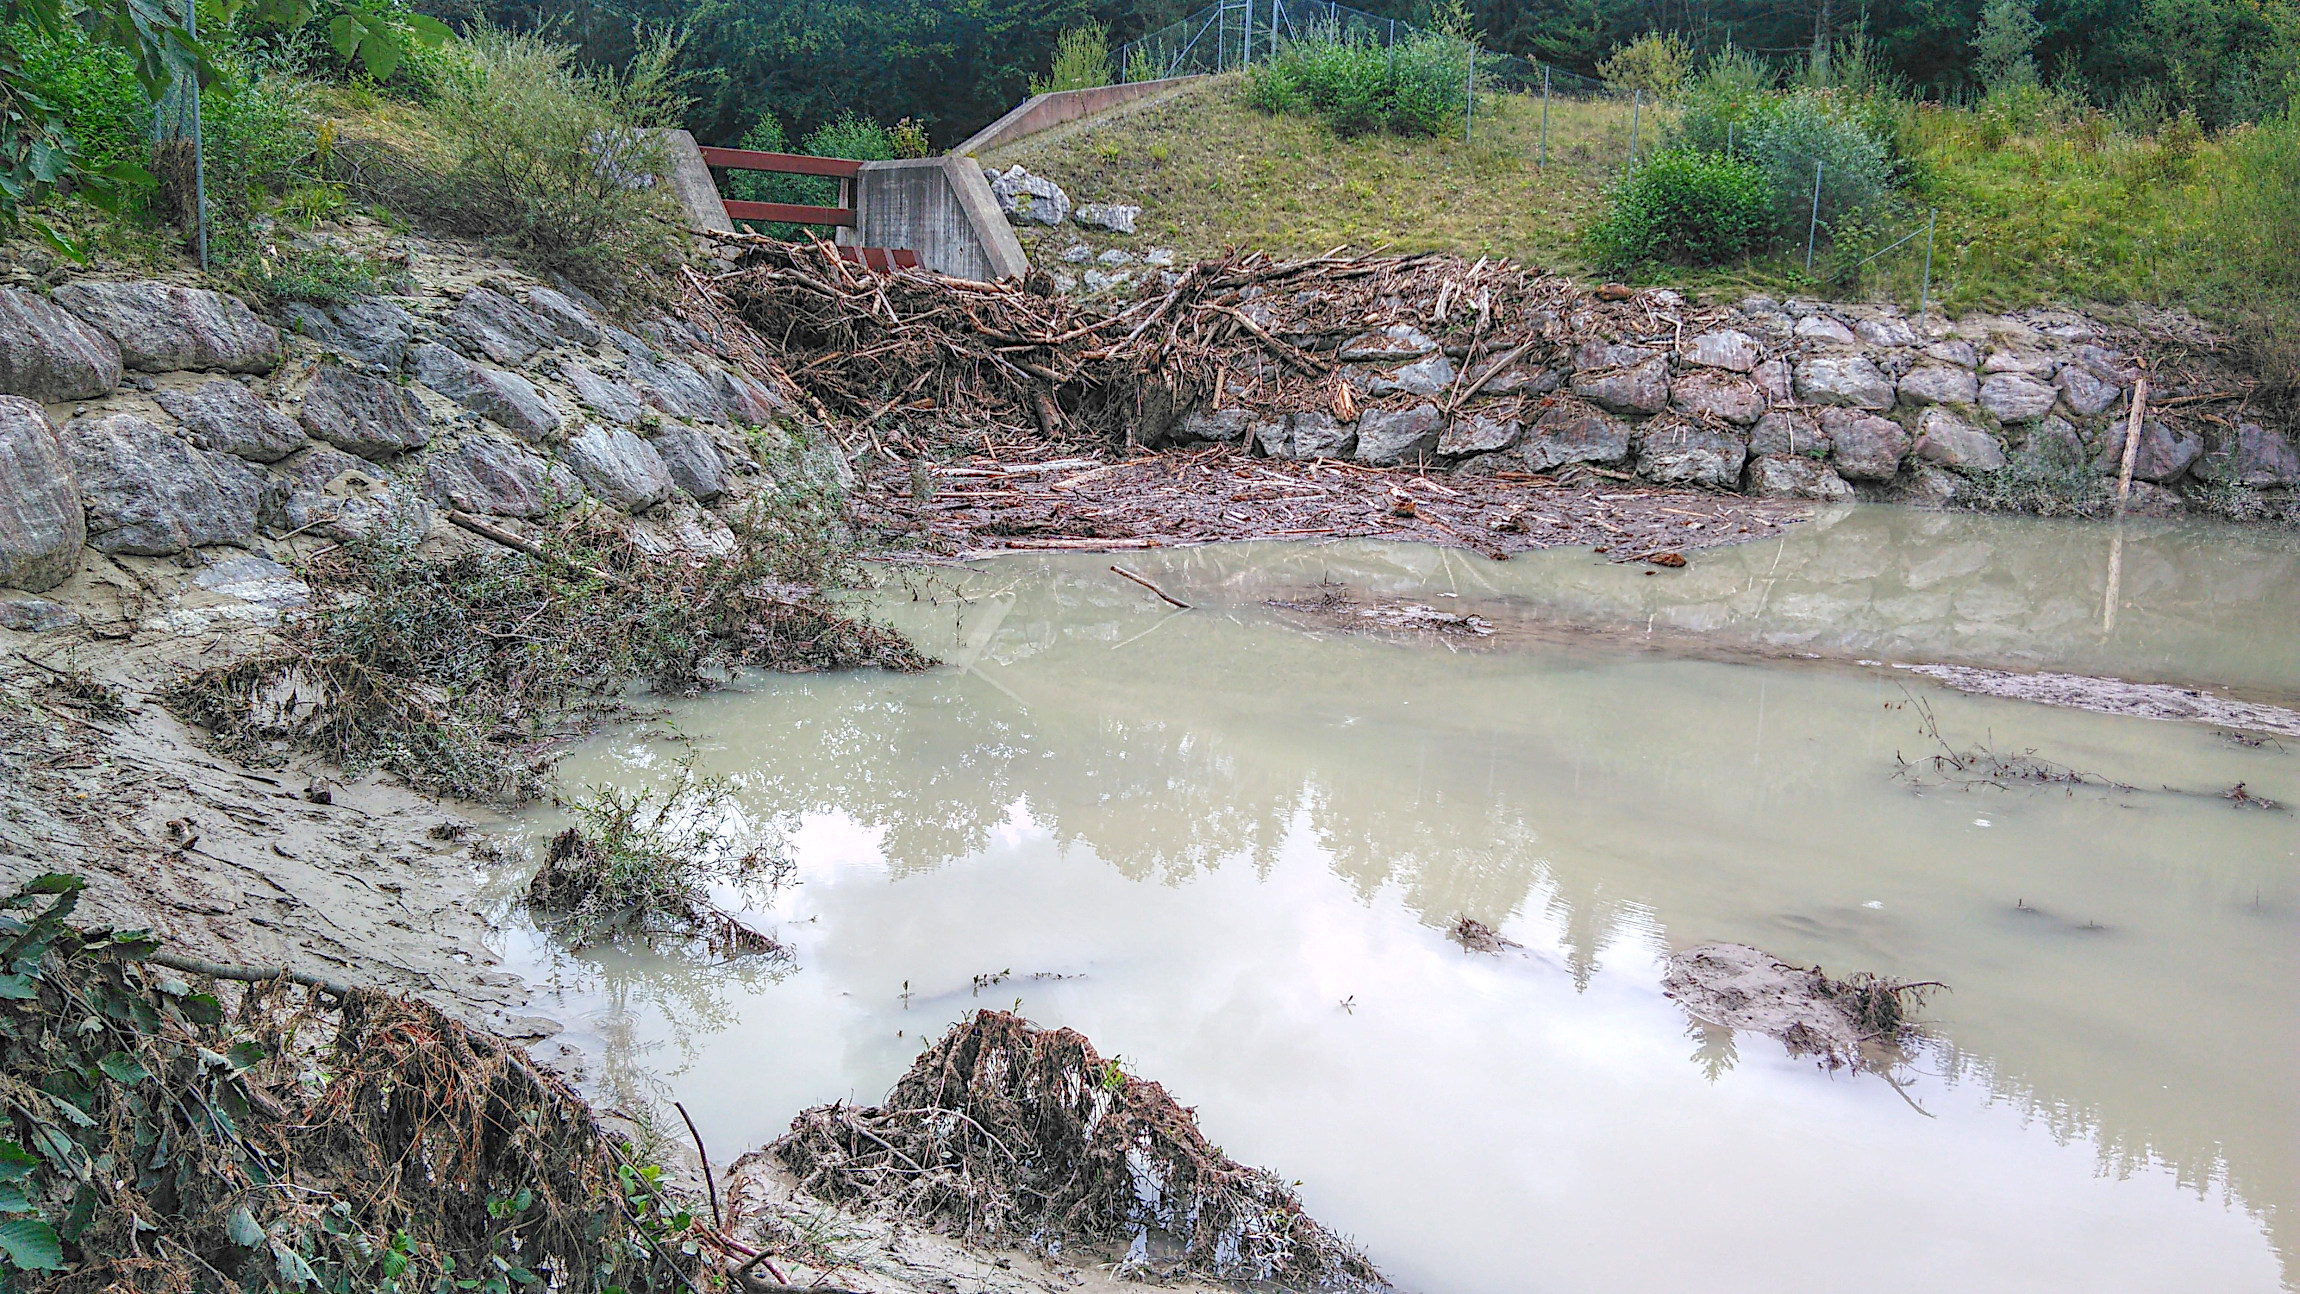
\includegraphics[width=0.865\paperwidth]{jenbach-trap-filled}};
		\end{scope}}
	\node[anchor=south west, xshift=0.33\paperwidth, yshift=2.13cm, text=black, text width=0.5\paperwidth,align=left]{\tiny \textcolor{gray}{Sediment trap at the Jenbach, Bavarian Alps}};
	\end{tikzpicture}
\end{frame}



\begin{frame}{\secname\vspace{0.1cm}\\\textcolor{anthrazit!80!white}{\subsecname}}
	\begin{tikzpicture}
		\clip (0,0) rectangle (\paperwidth,\paperheight);
		\onslide<1->{
			\begin{scope}
				\node[anchor=south west, xshift=0.0\paperwidth, yshift=0.34\paperheight] {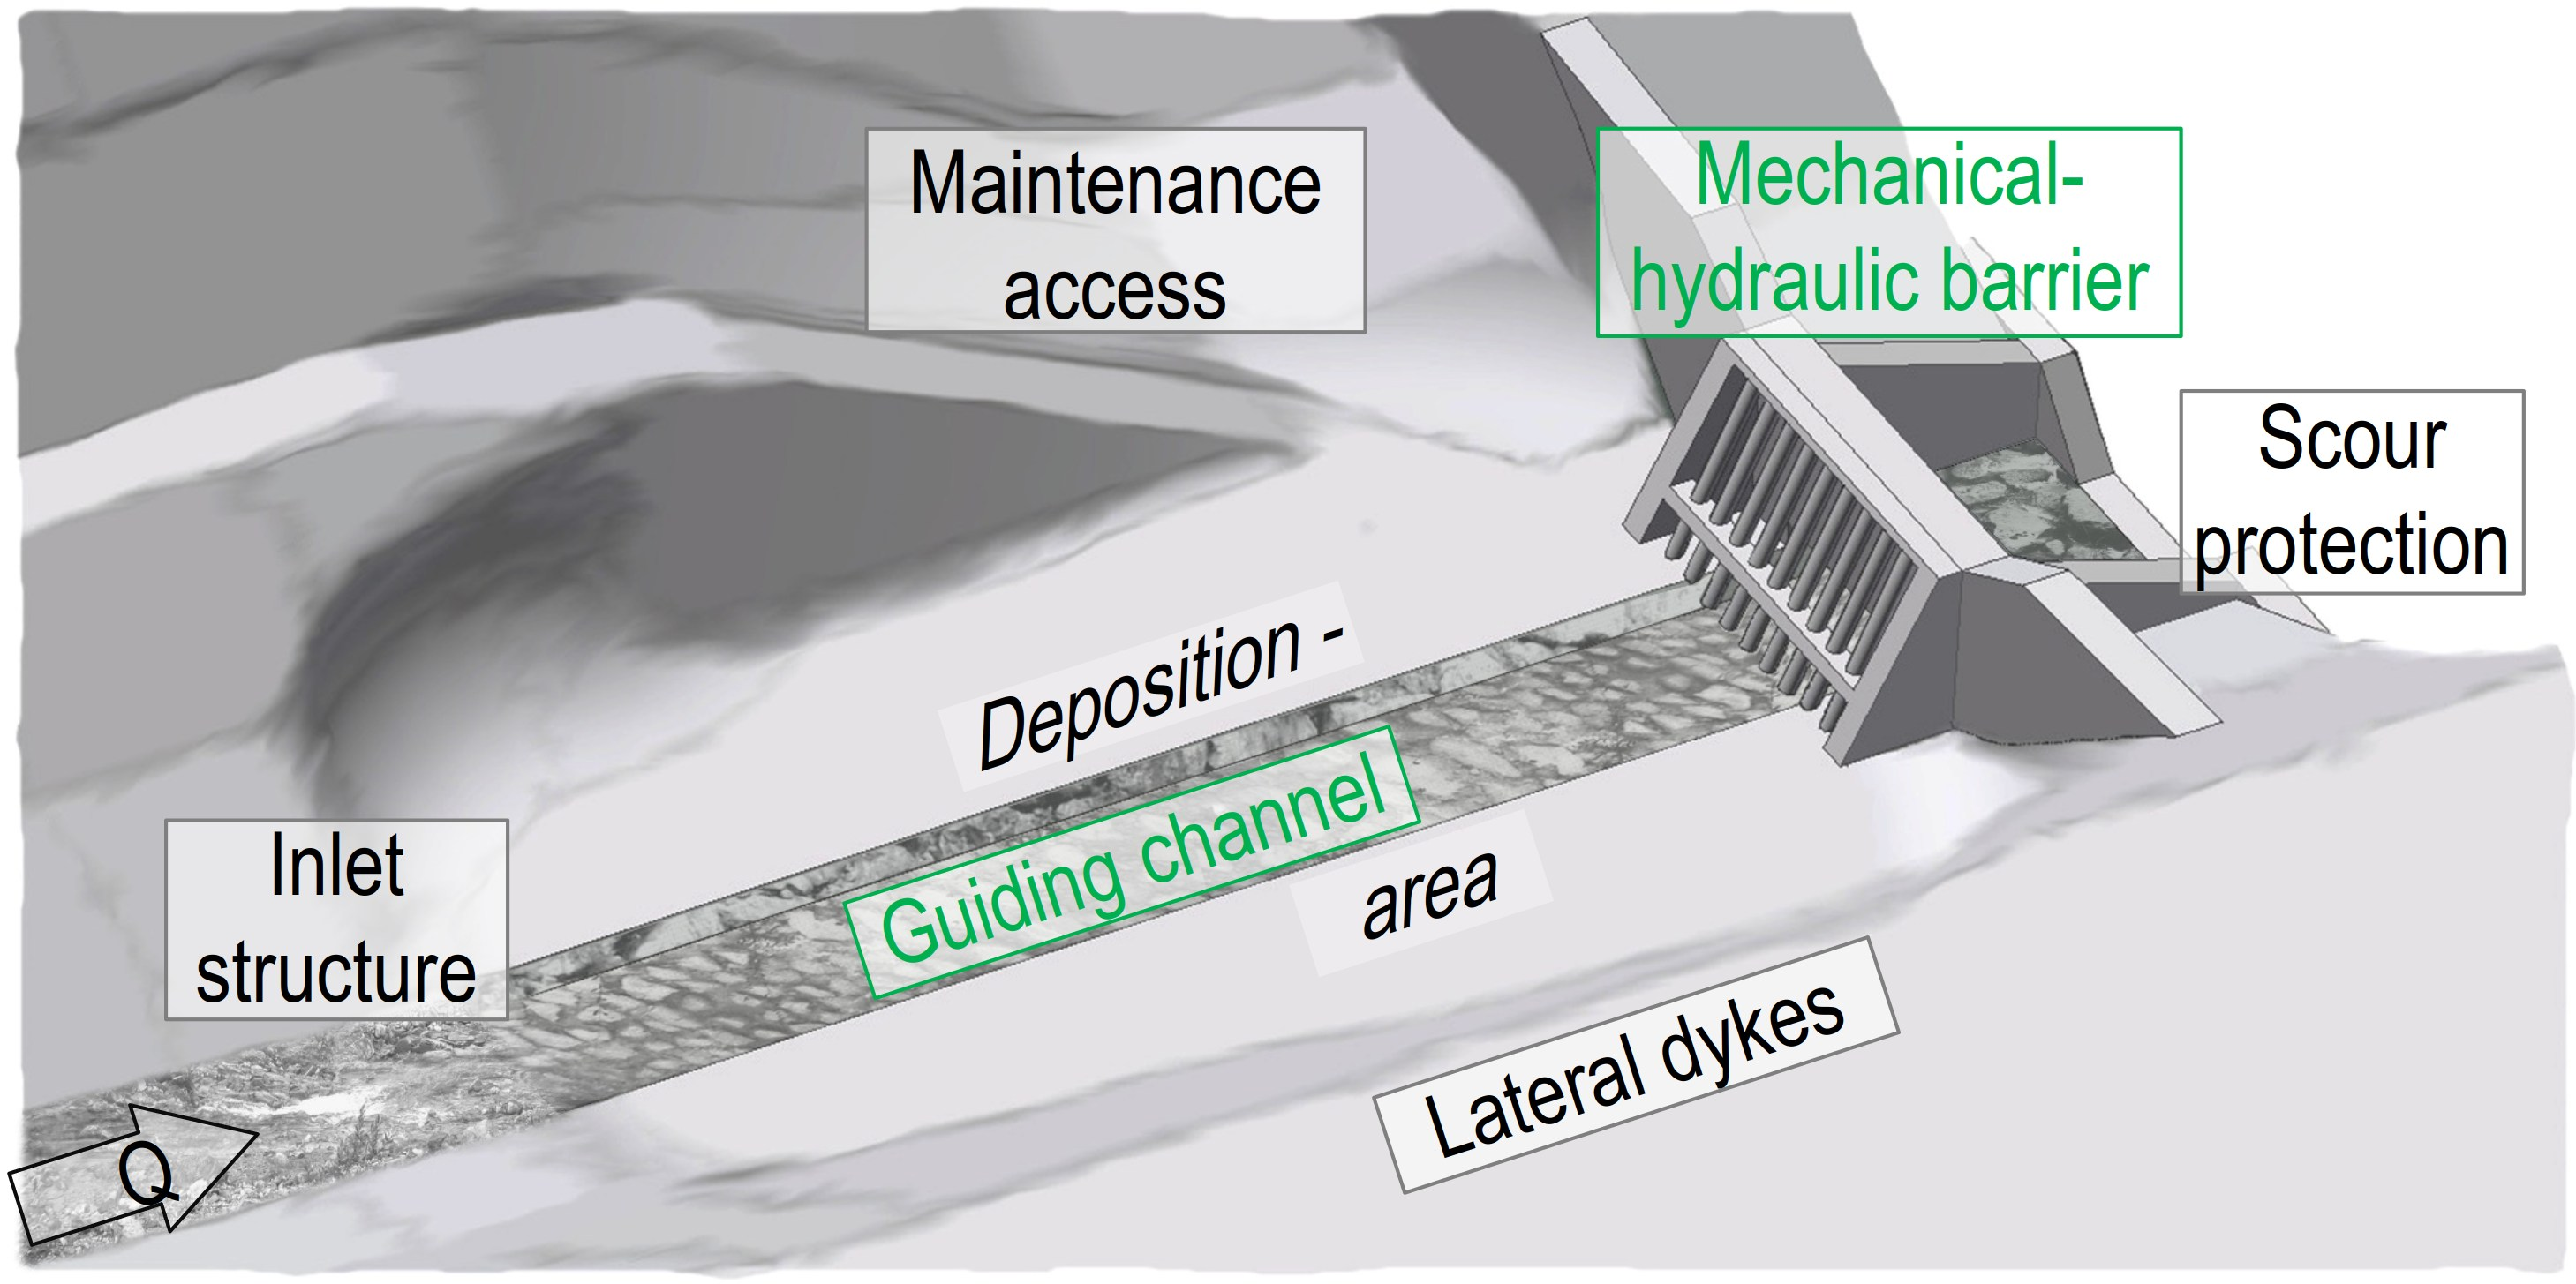
\includegraphics[width=0.88	\paperwidth]{check-dam-concept}};
		\end{scope}}
		\onslide<1-1>{
			\node[anchor=south west, xshift=0.21\paperwidth, yshift=2.21cm, text=black, text width=0.55\paperwidth,align=left]{\tiny \textcolor{gray}{Source: \sscURL{Schwindt \textit{et al.} (2018)}{https://www.nat-hazards-earth-syst-sci.net/18/647/2018/} / \sscURL{Moldenhauer, Piton, Schwindt \textit{et al. (2021)}}{https://www.sciencedirect.com/science/article/pii/S1001627920300792}}};}
	\end{tikzpicture}
\end{frame}

\subsection{Sediment Management in Reservoirs}

\begin{frame}{\secname\vspace{0.1cm}\\\textcolor{anthrazit!80!white}{\subsecname}}
	\begin{tikzpicture}
		\clip (0,0) rectangle (\paperwidth,\paperheight);
		\onslide<1->{
			\begin{scope}
				\node[anchor=south west, xshift=0.0\paperwidth, yshift=0.48\paperheight] {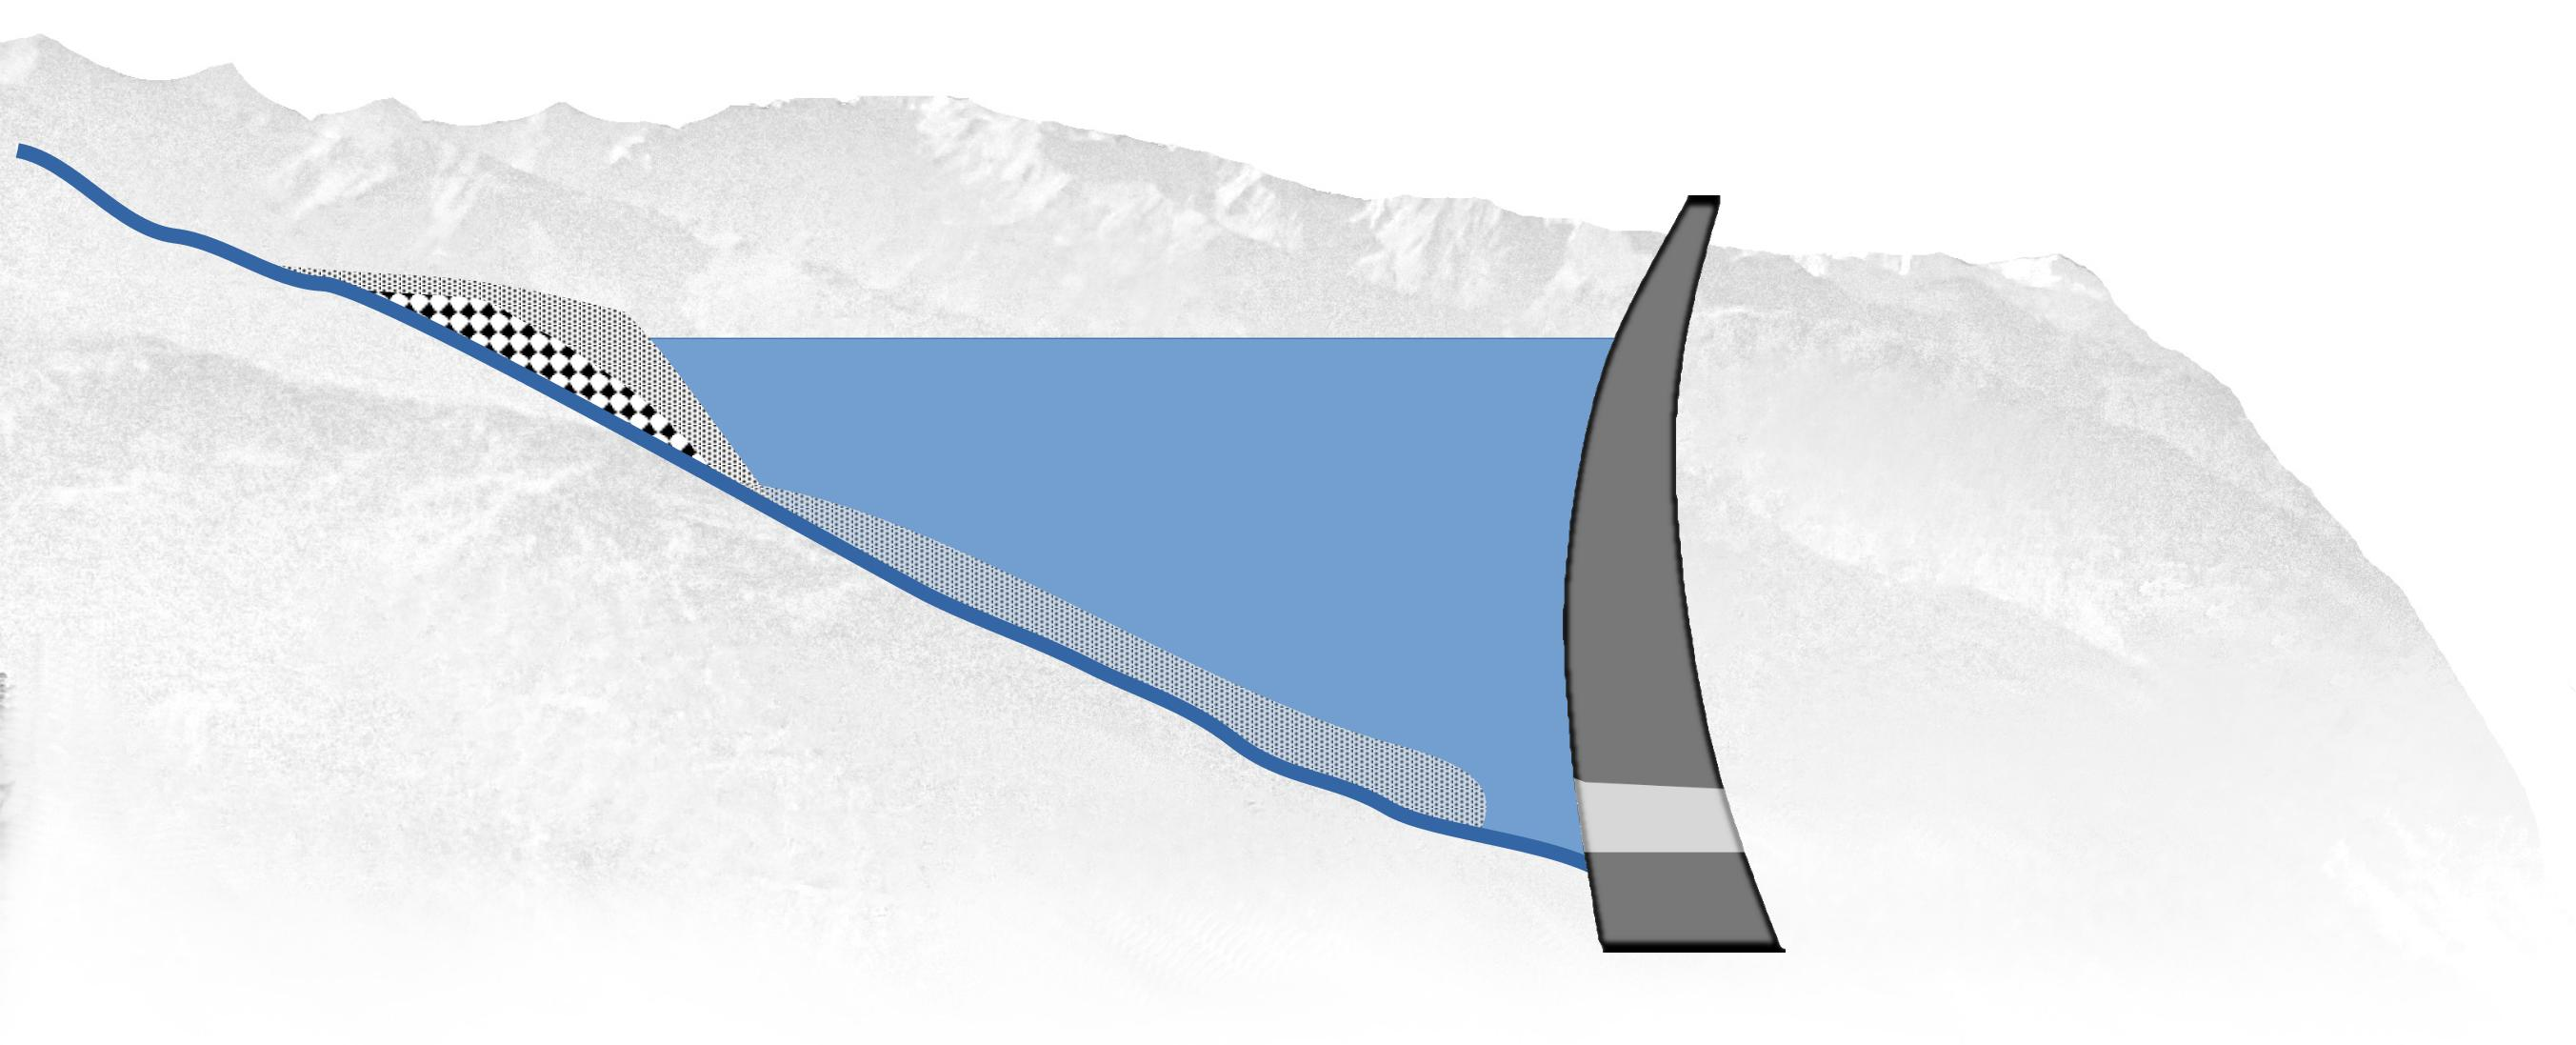
\includegraphics[width=0.91\paperwidth]{dam-scheme-zoom}};
		\end{scope}}
%		\onslide<2->{
%			\begin{scope}
%				\node[anchor=south west, xshift=0.0\paperwidth, yshift=0.48\paperheight] {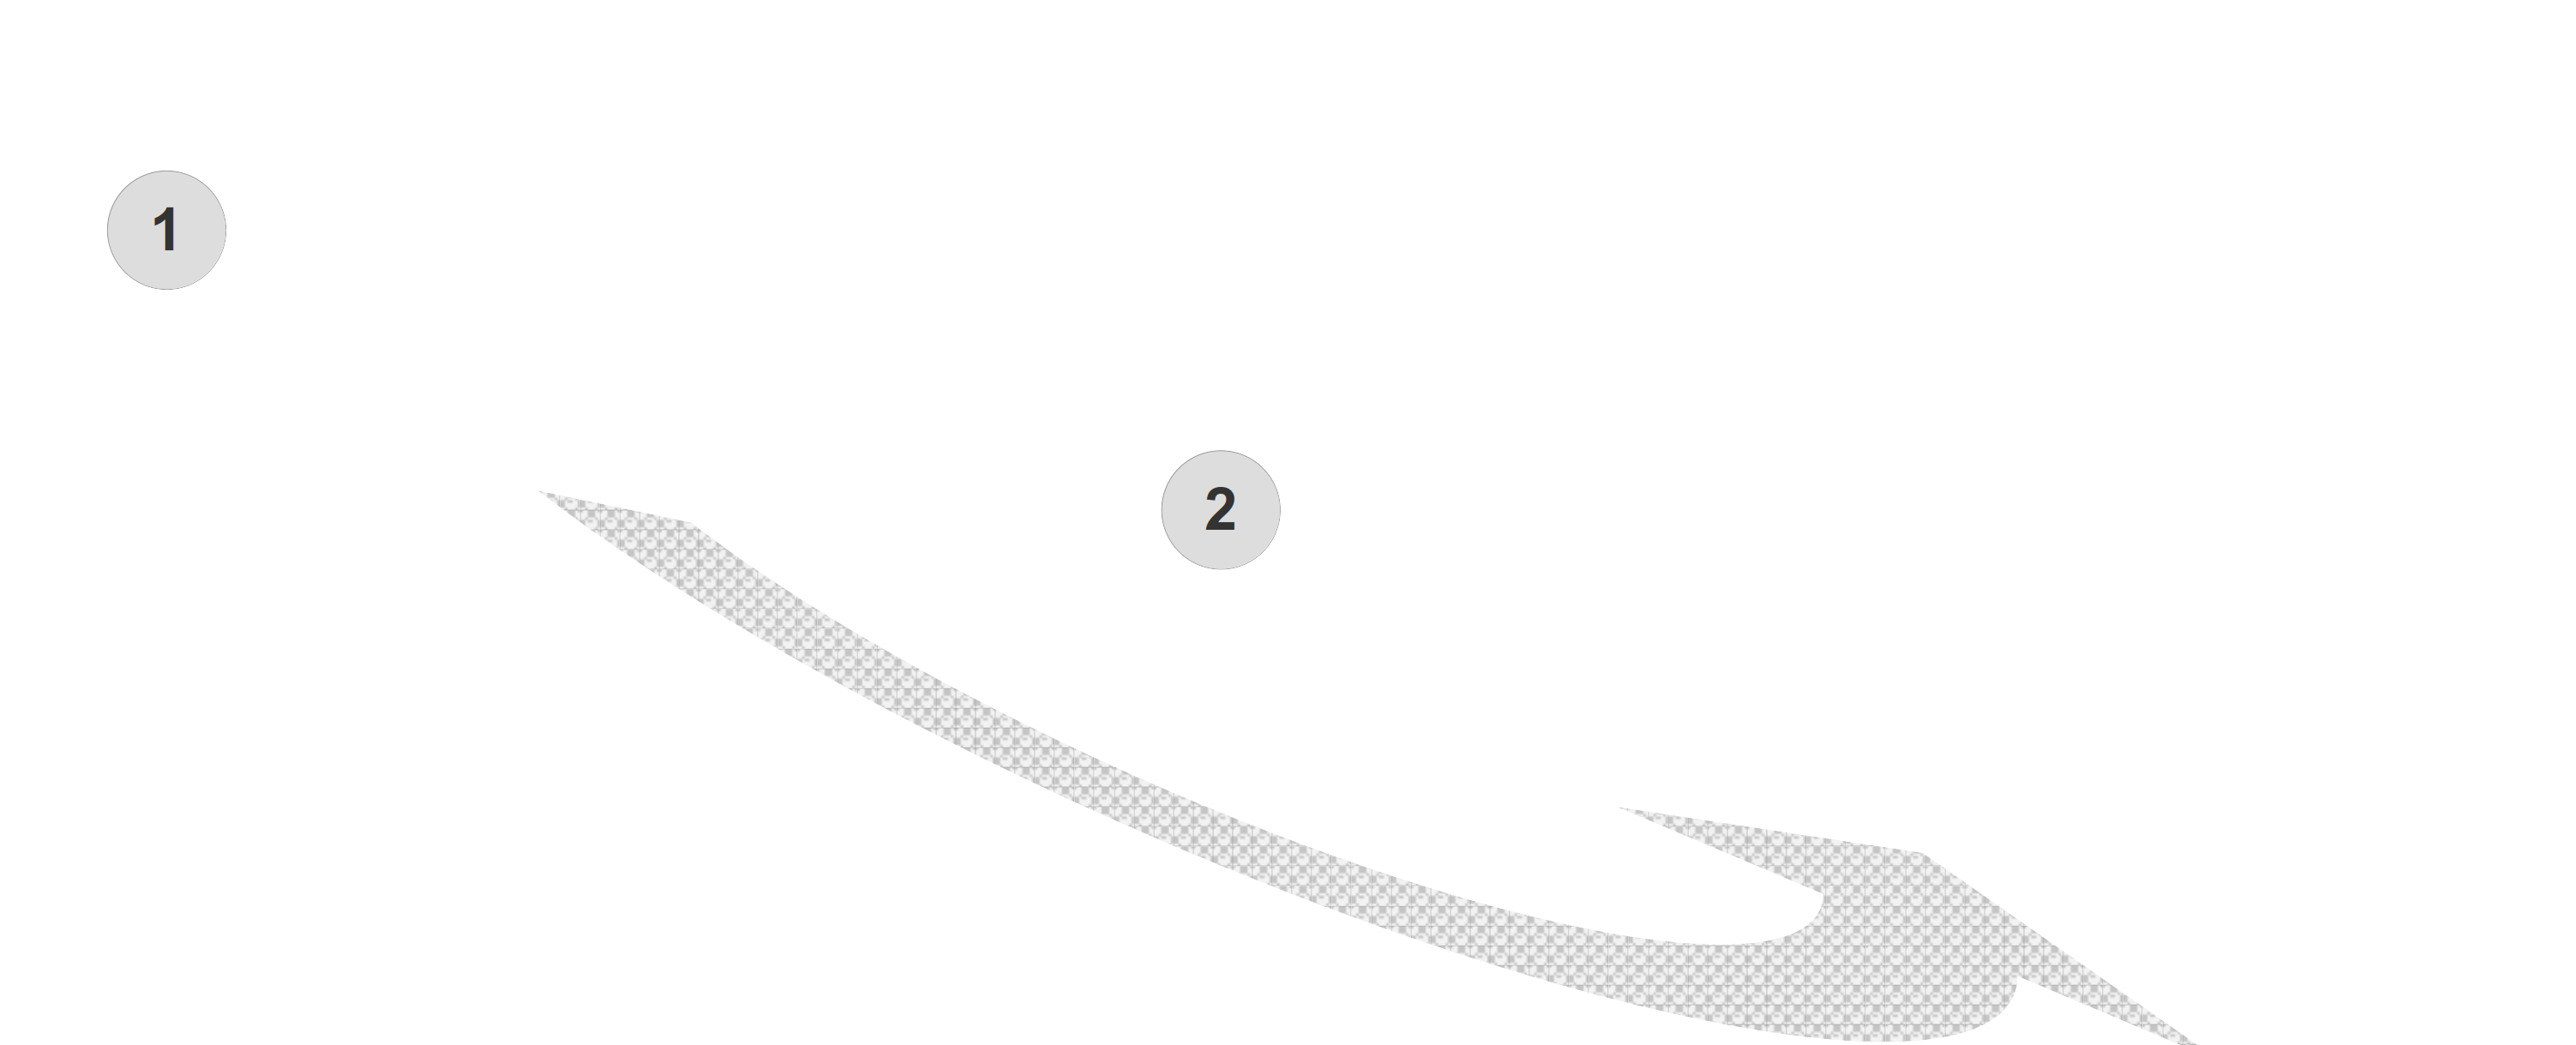
\includegraphics[width=0.91\paperwidth]{dam-scheme-zoom-overlay}};
%		\end{scope}}
		\onslide<1->{
			\begin{scope}
				\node[anchor=south west, xshift=0.0\paperwidth, yshift=0.32\paperheight] {
					\begin{minipage}{0.95\textwidth}
						\begin{itemize}
							% \setlength\itemsep{0.7em}
							\item[\faHandORight]\ Coarse \& fine sediment deposits in delta regions (reservoir head)
							\item[\faHandORight]\ Very fine, partially cohesive sediment disperses in the entire reservoir
							\item[\faHandORight]\ Turbidity currents move suspended sediment close to dams
						\end{itemize}
					\end{minipage}
				};
		\end{scope}}
		\onslide<1->{
			\node[anchor=south west, xshift=0.33\paperwidth, yshift=2.1947cm, text=black, text width=0.5\paperwidth,align=left]{\tiny \textcolor{gray}{Image concept from Chamoun \textit{et al.} (2017) / SCCER-SoE}};}
	\end{tikzpicture}
\end{frame}

\begin{frame}{\secname\vspace{0.1cm}\\\textcolor{anthrazit!80!white}{\subsecname}}
	\begin{tikzpicture}
		\clip (0,0) rectangle (\paperwidth,\paperheight);
		\onslide<1->{
			\begin{scope}
				\node[anchor=south west, xshift=0.06\paperwidth, yshift=0.27\paperheight] {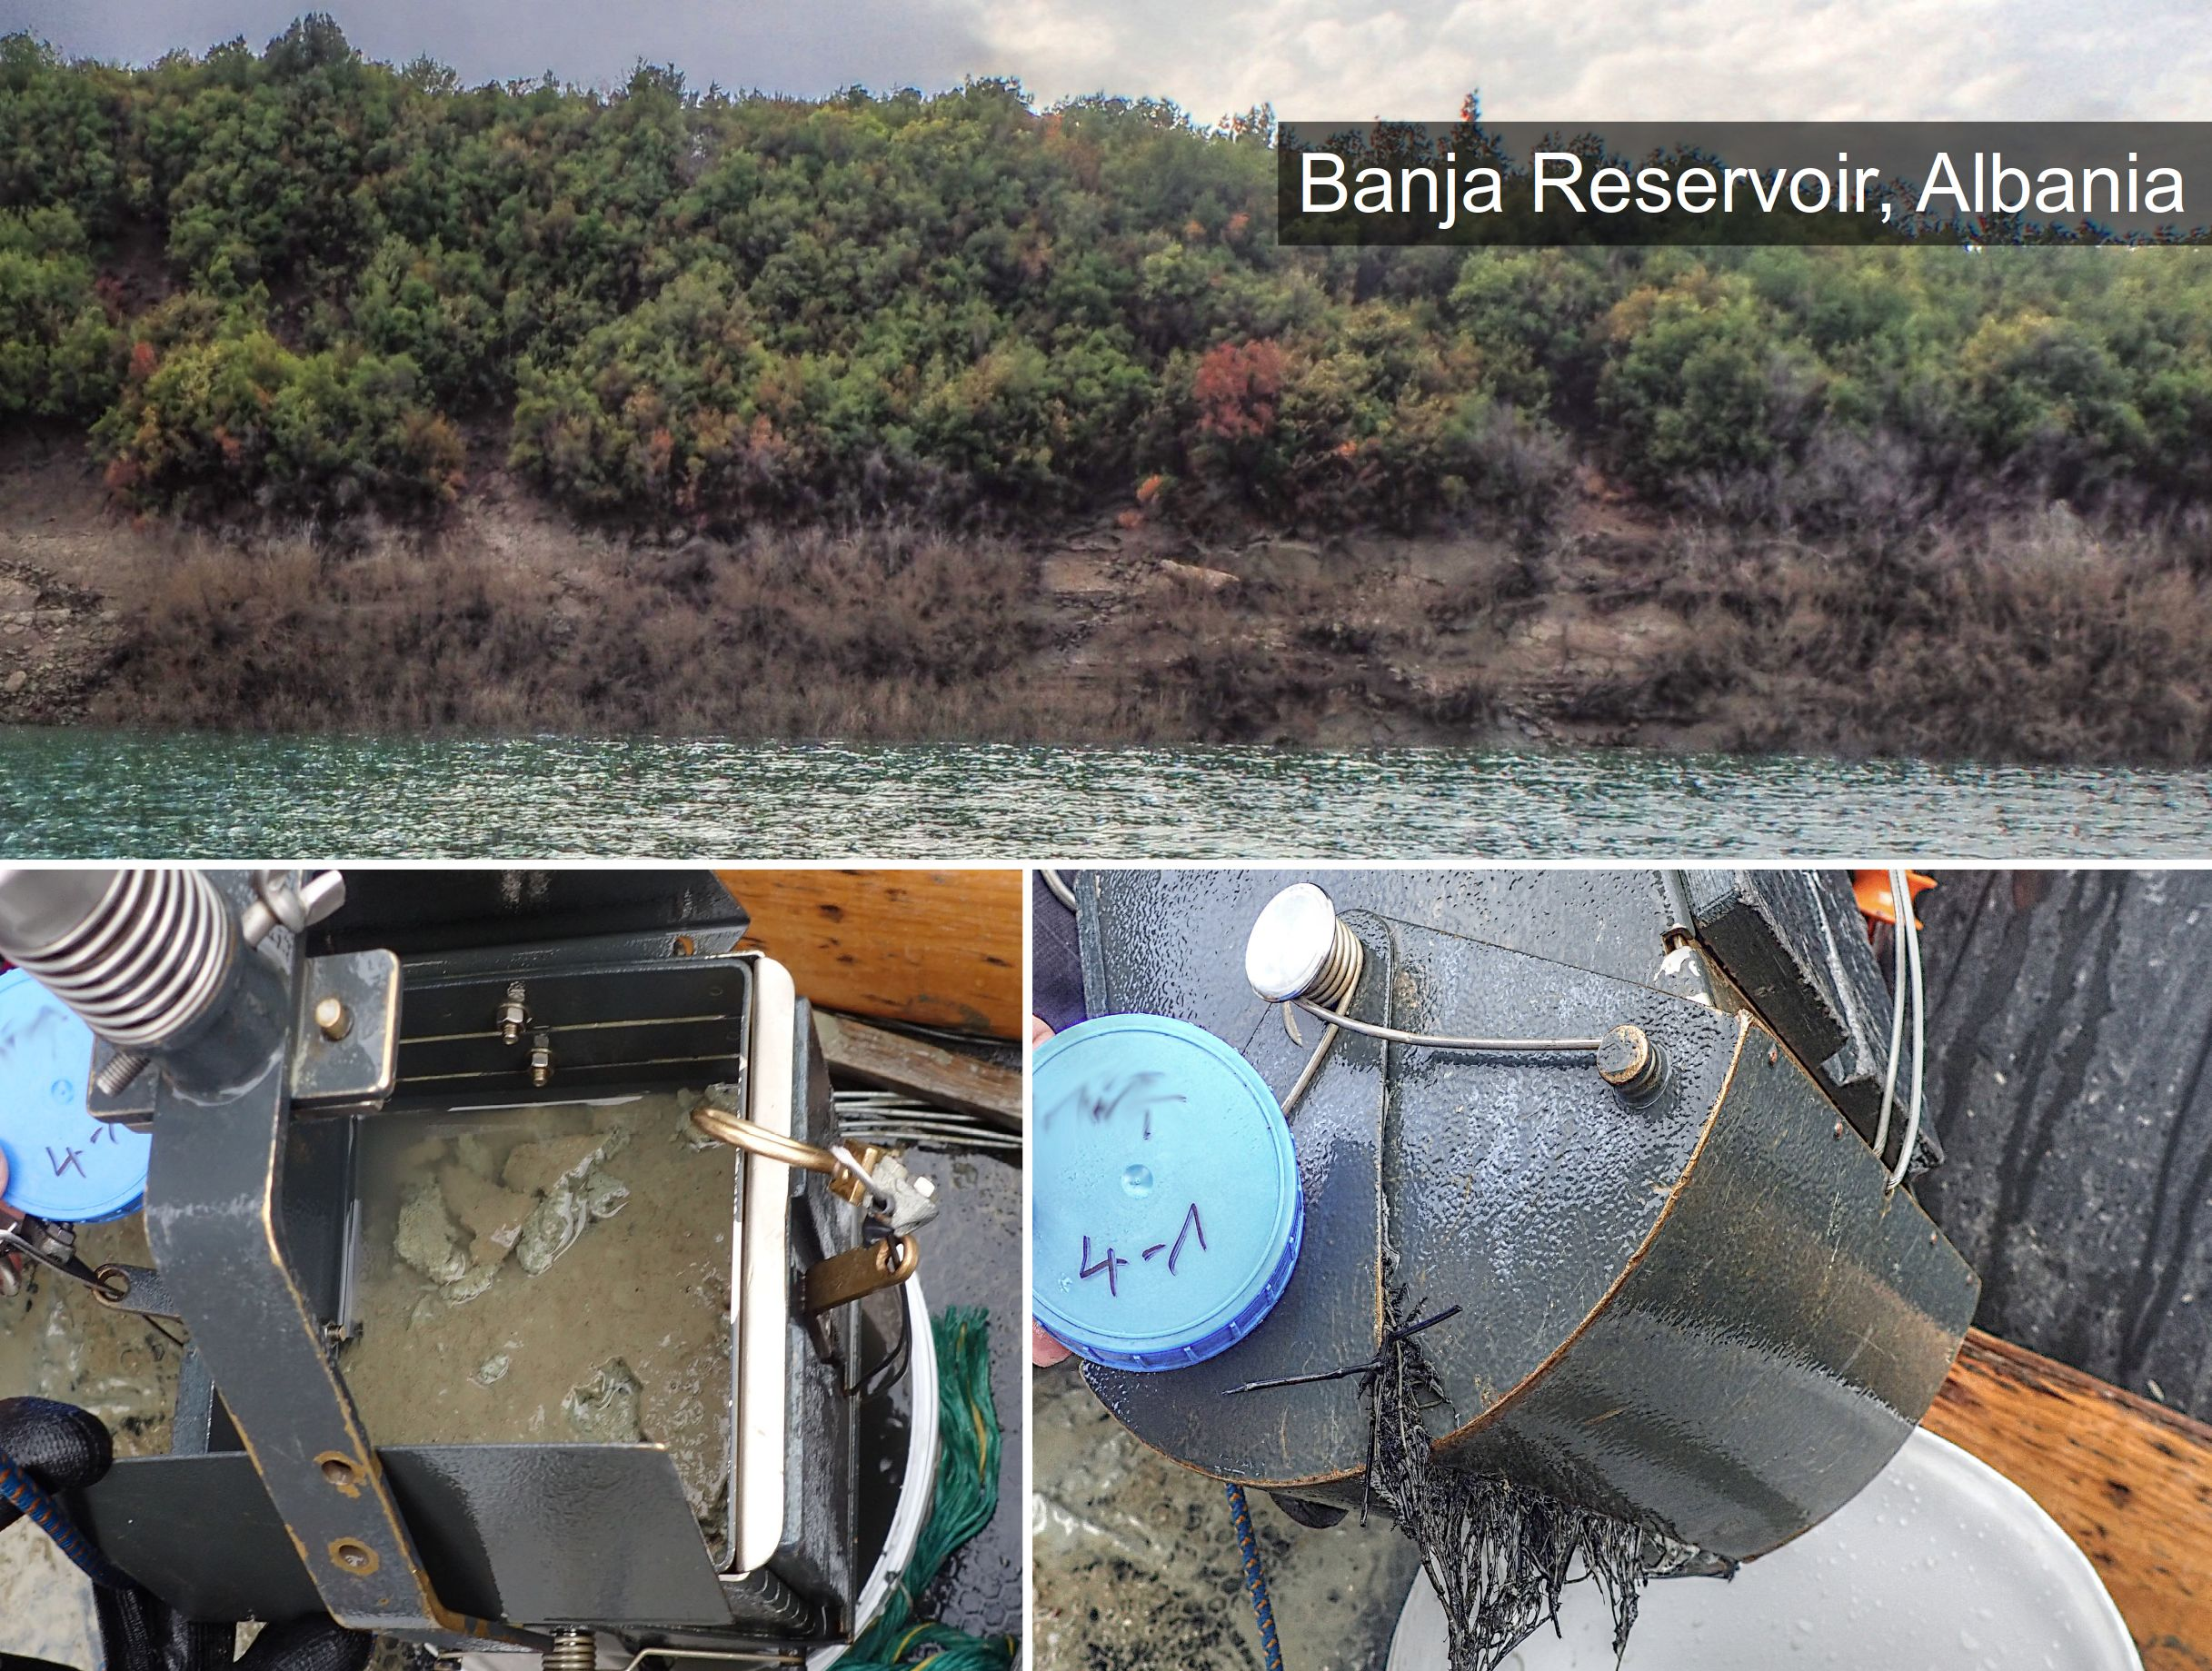
\includegraphics[width=0.73\paperwidth]{banja-mud}};
		\end{scope}}
	\end{tikzpicture}
\end{frame}

\begin{frame}{\secname\vspace{0.1cm}\\\textcolor{anthrazit!80!white}{\subsecname}}
	\begin{tikzpicture}
		\clip (0,0) rectangle (\paperwidth,\paperheight);
		\onslide<1->{
		\begin{scope}
			\node[anchor=south west, xshift=0.05\paperwidth, yshift=0.4\paperheight] {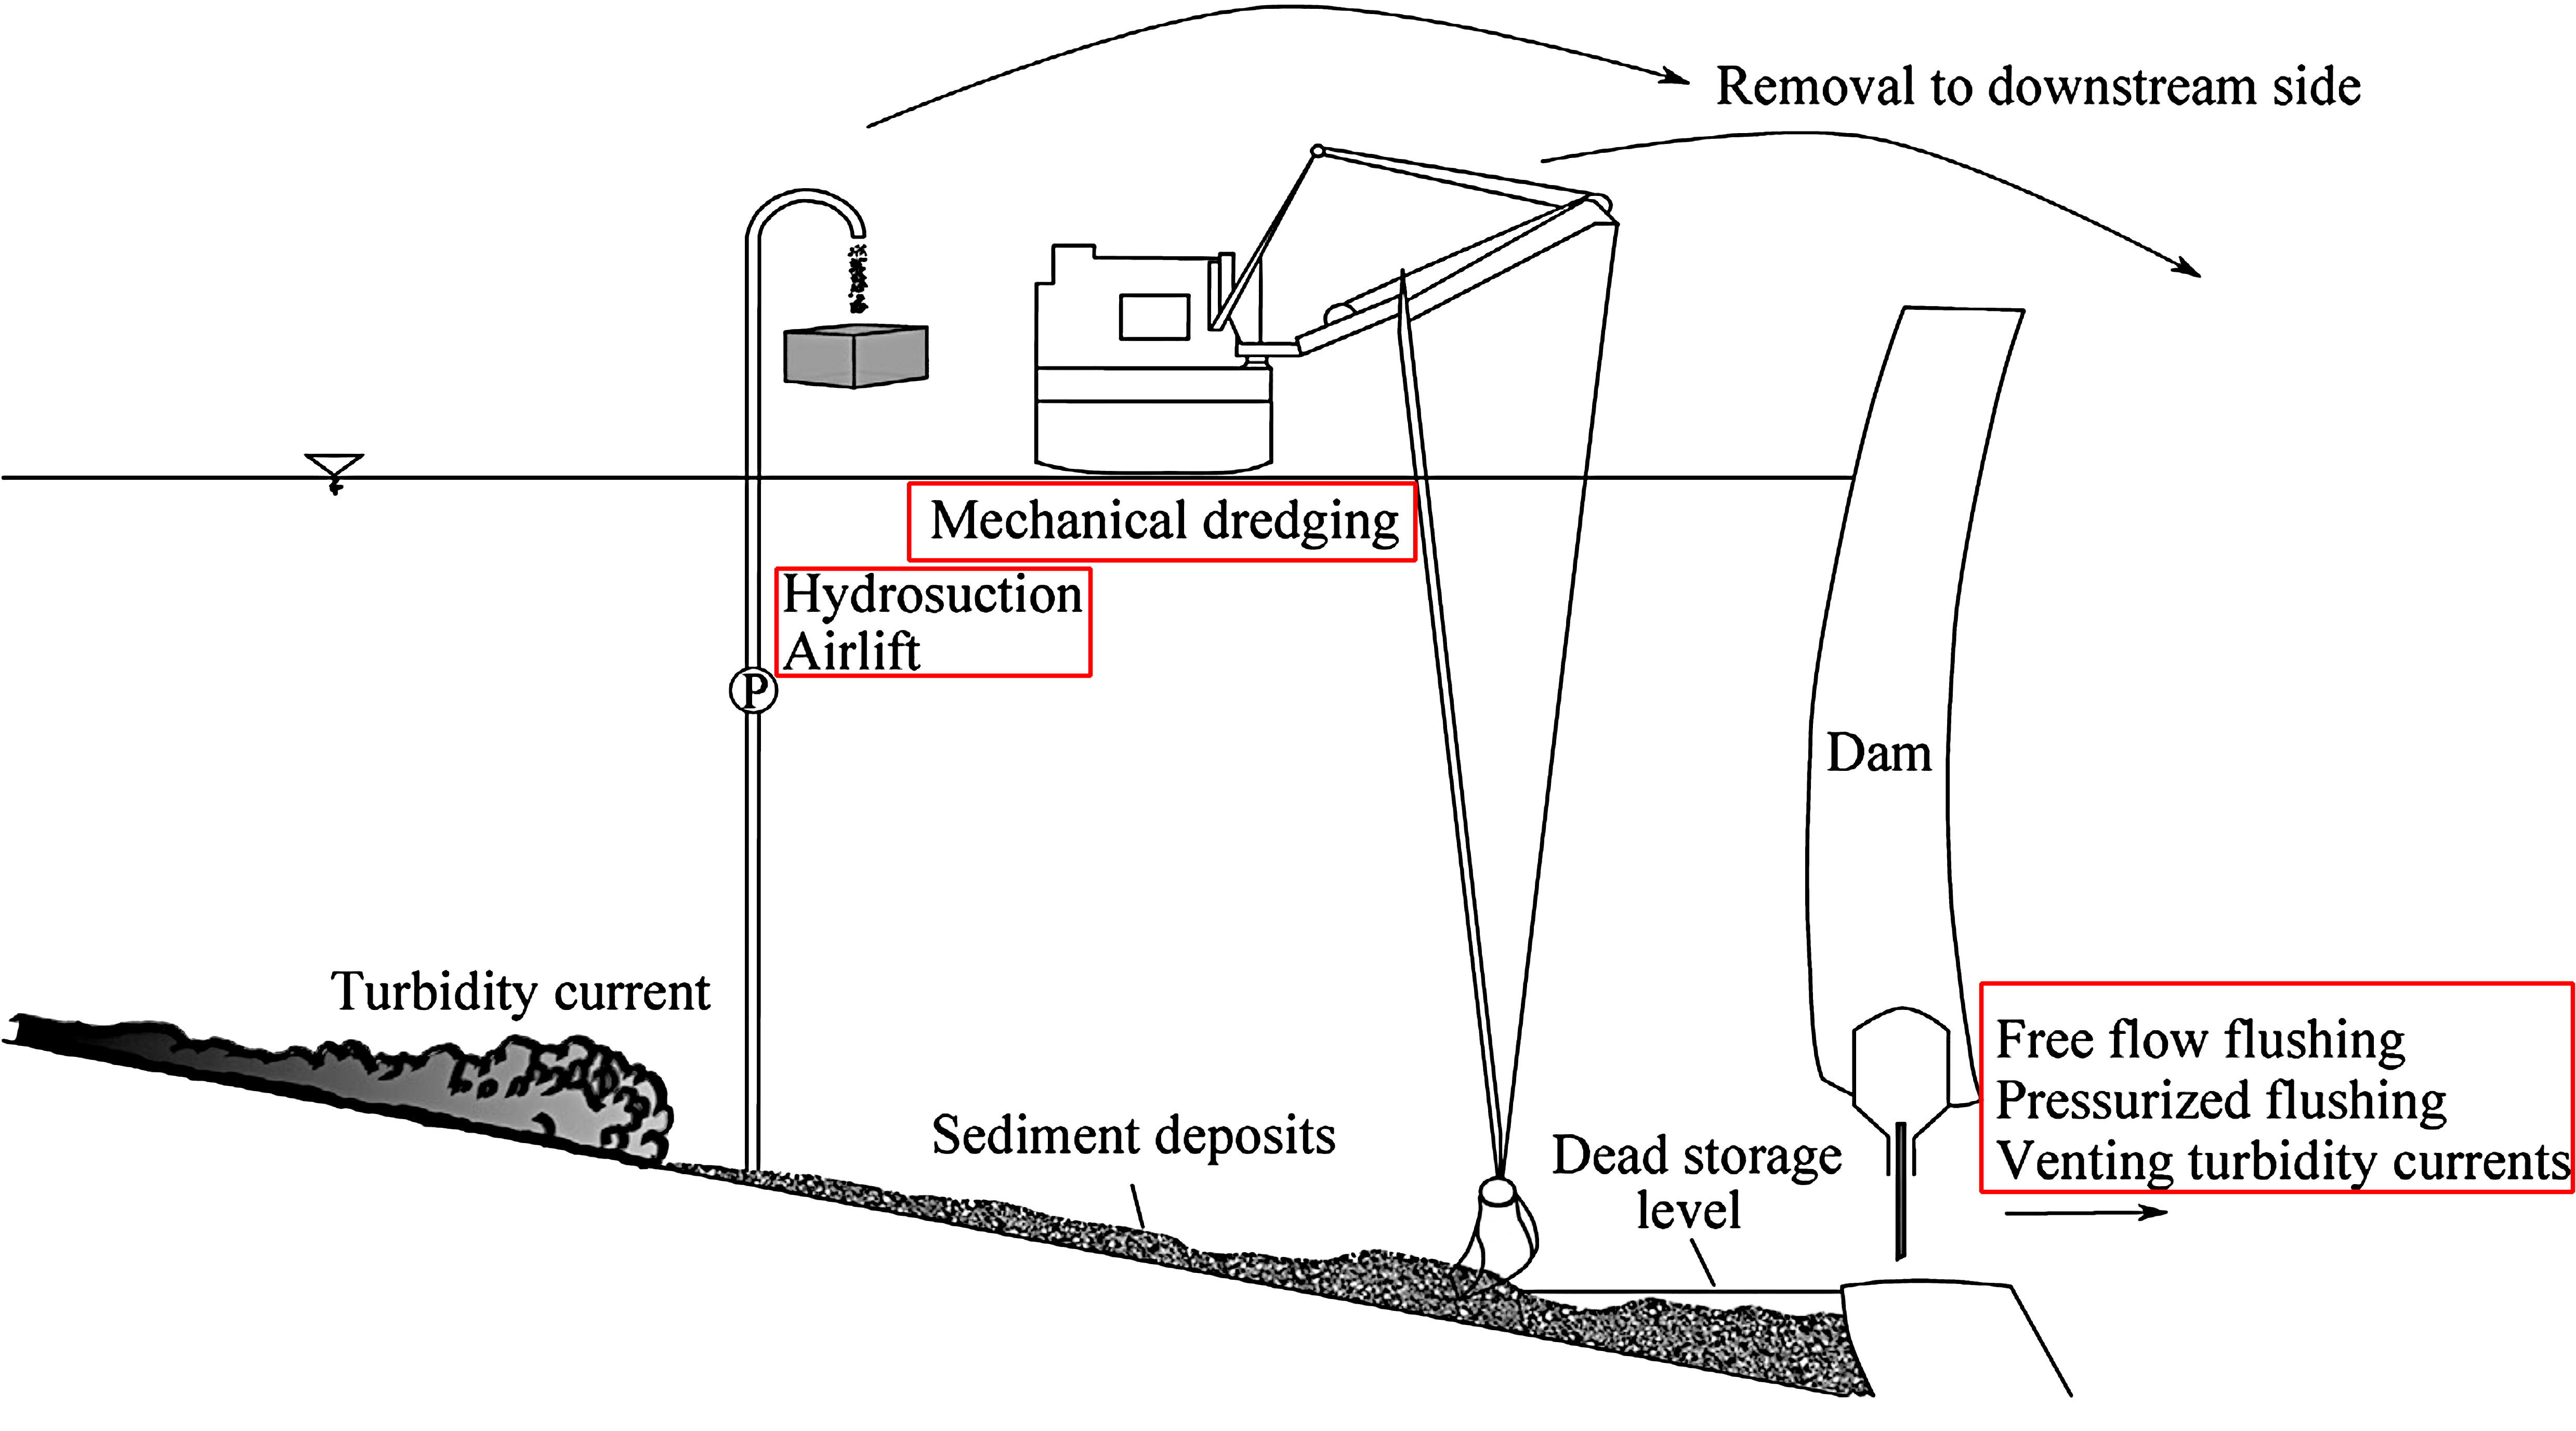
\includegraphics[width=0.78	\paperwidth]{reservoir-sedimentation-mgmt-highlight}};
		\end{scope}}
		\onslide<1->{
		\begin{scope}
			\node[anchor=south west, xshift=0.0\paperwidth, yshift=0.3\paperheight] {
				\begin{minipage}{0.95\textwidth}
					\begin{itemize}
						\item[\faHandORight]\ Airlift / hydrosuction
						\item[\faHandORight]\ Mechanical dredging
						\item[\faHandORight]\ Flushing (free flow, pressurized, venting) \& re-suspension
						\item[\faHandORight]\ Sediment bypass tunnels
					\end{itemize}
				\end{minipage}
			};
		\end{scope}}
		\onslide<1-1>{
			\node[anchor=south west, xshift=0.33\paperwidth, yshift=2.13cm, text=black, text width=0.5\paperwidth,align=left]{\tiny \textcolor{gray}{Source: Chamoun \textit{et al.} / SCCER-SoE (2018)}};}
	\end{tikzpicture}
\end{frame}

\begin{frame}{\secname\vspace{0.1cm}\\\textcolor{anthrazit!80!white}{\subsecname}}
	\begin{center}
		\movie[externalviewer]{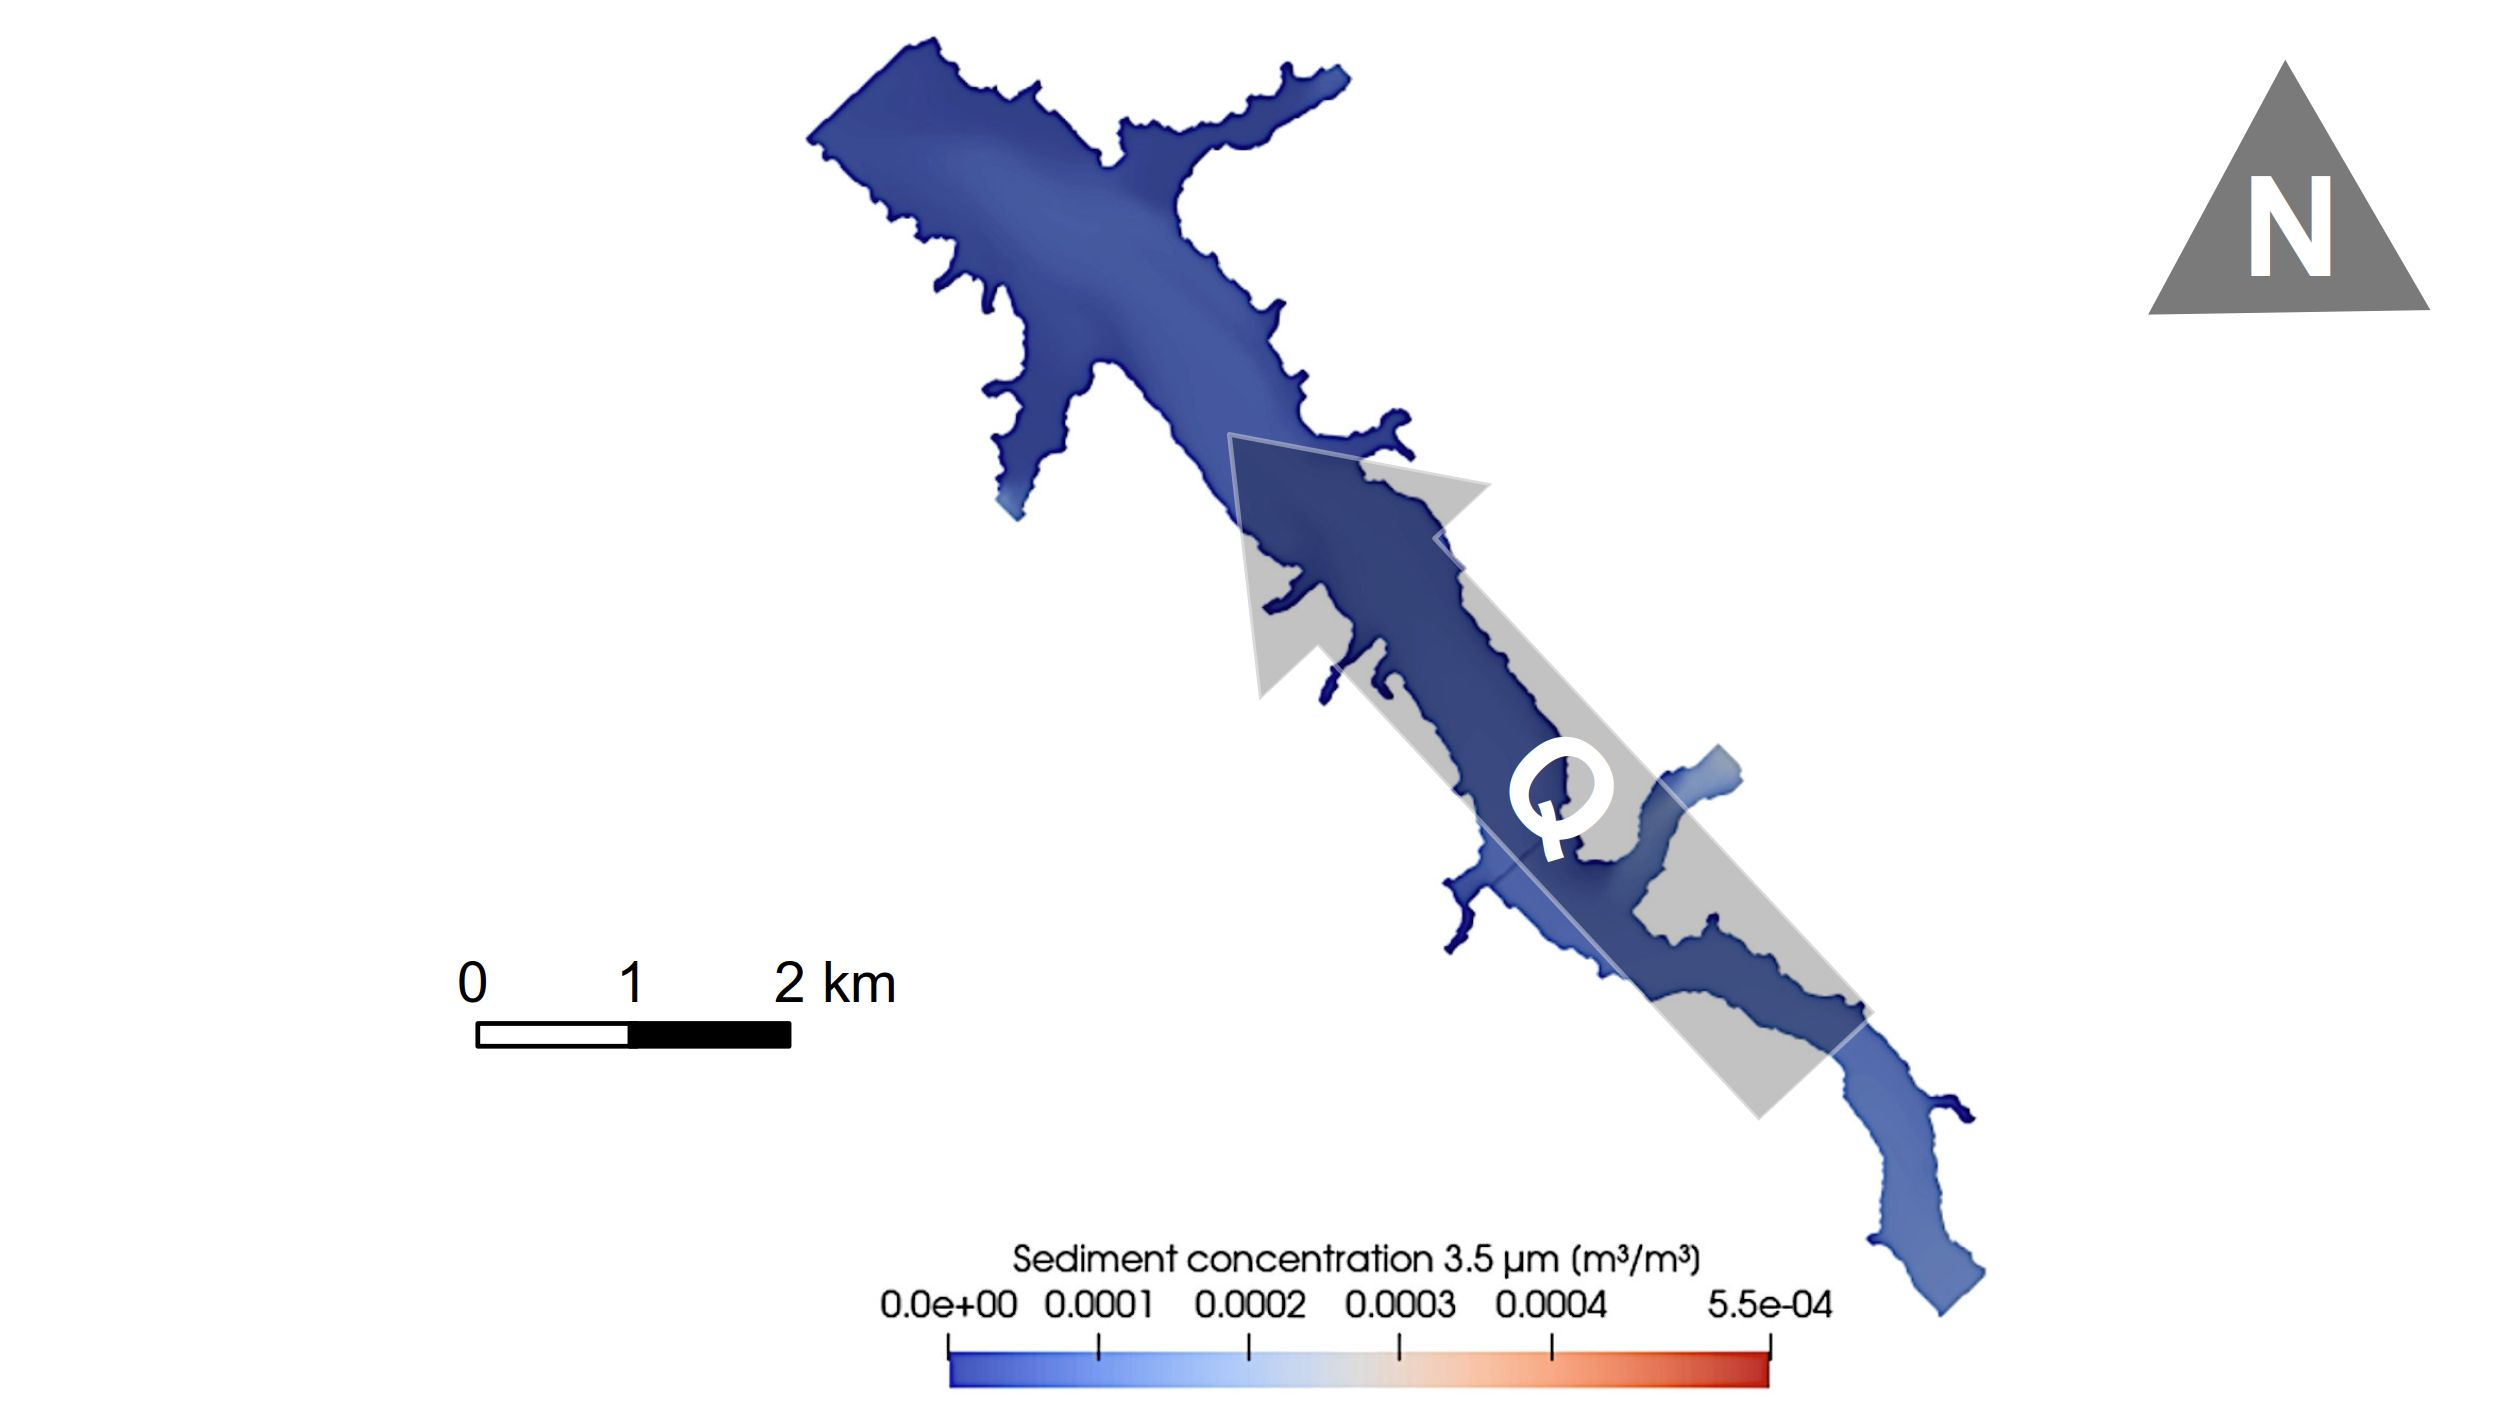
\includegraphics[width=0.95\textwidth,keepaspectratio]{videos/thumbnail-sed-conc.jpg}}{videos/sed-conc.avi}\\
		\textit{Fine particle transport through the Banja reservoir 2016--2019\\
			\textcolor{gray}{(\sscURL{Mouris \textit{et al.}, 2023a}{https://doi.org/10.1007/s40808-023-01712-7}, \sscURL{Mouris \textit{et al.}, 2023b}{https://www.nature.com/articles/s41598-023-47501-1})}}
	\end{center}
\end{frame}

\section{Vertical \& Lateral Connectivity {
\includegraphics[height=15pt]{connectivity-yz-small}}}

\subsection{Vertical Disconnectivity: Riverbed Clogging}

\begin{frame}{\secname\vspace{0.1cm}\\\textcolor{anthrazit!80!white}{\subsecname}}
	\begin{tikzpicture}
		\clip (0,0) rectangle (\paperwidth,\paperheight);
		\onslide<1->{
		\begin{scope}
				\node[anchor=south west, xshift=0.0\paperwidth, yshift=0.62\paperheight] {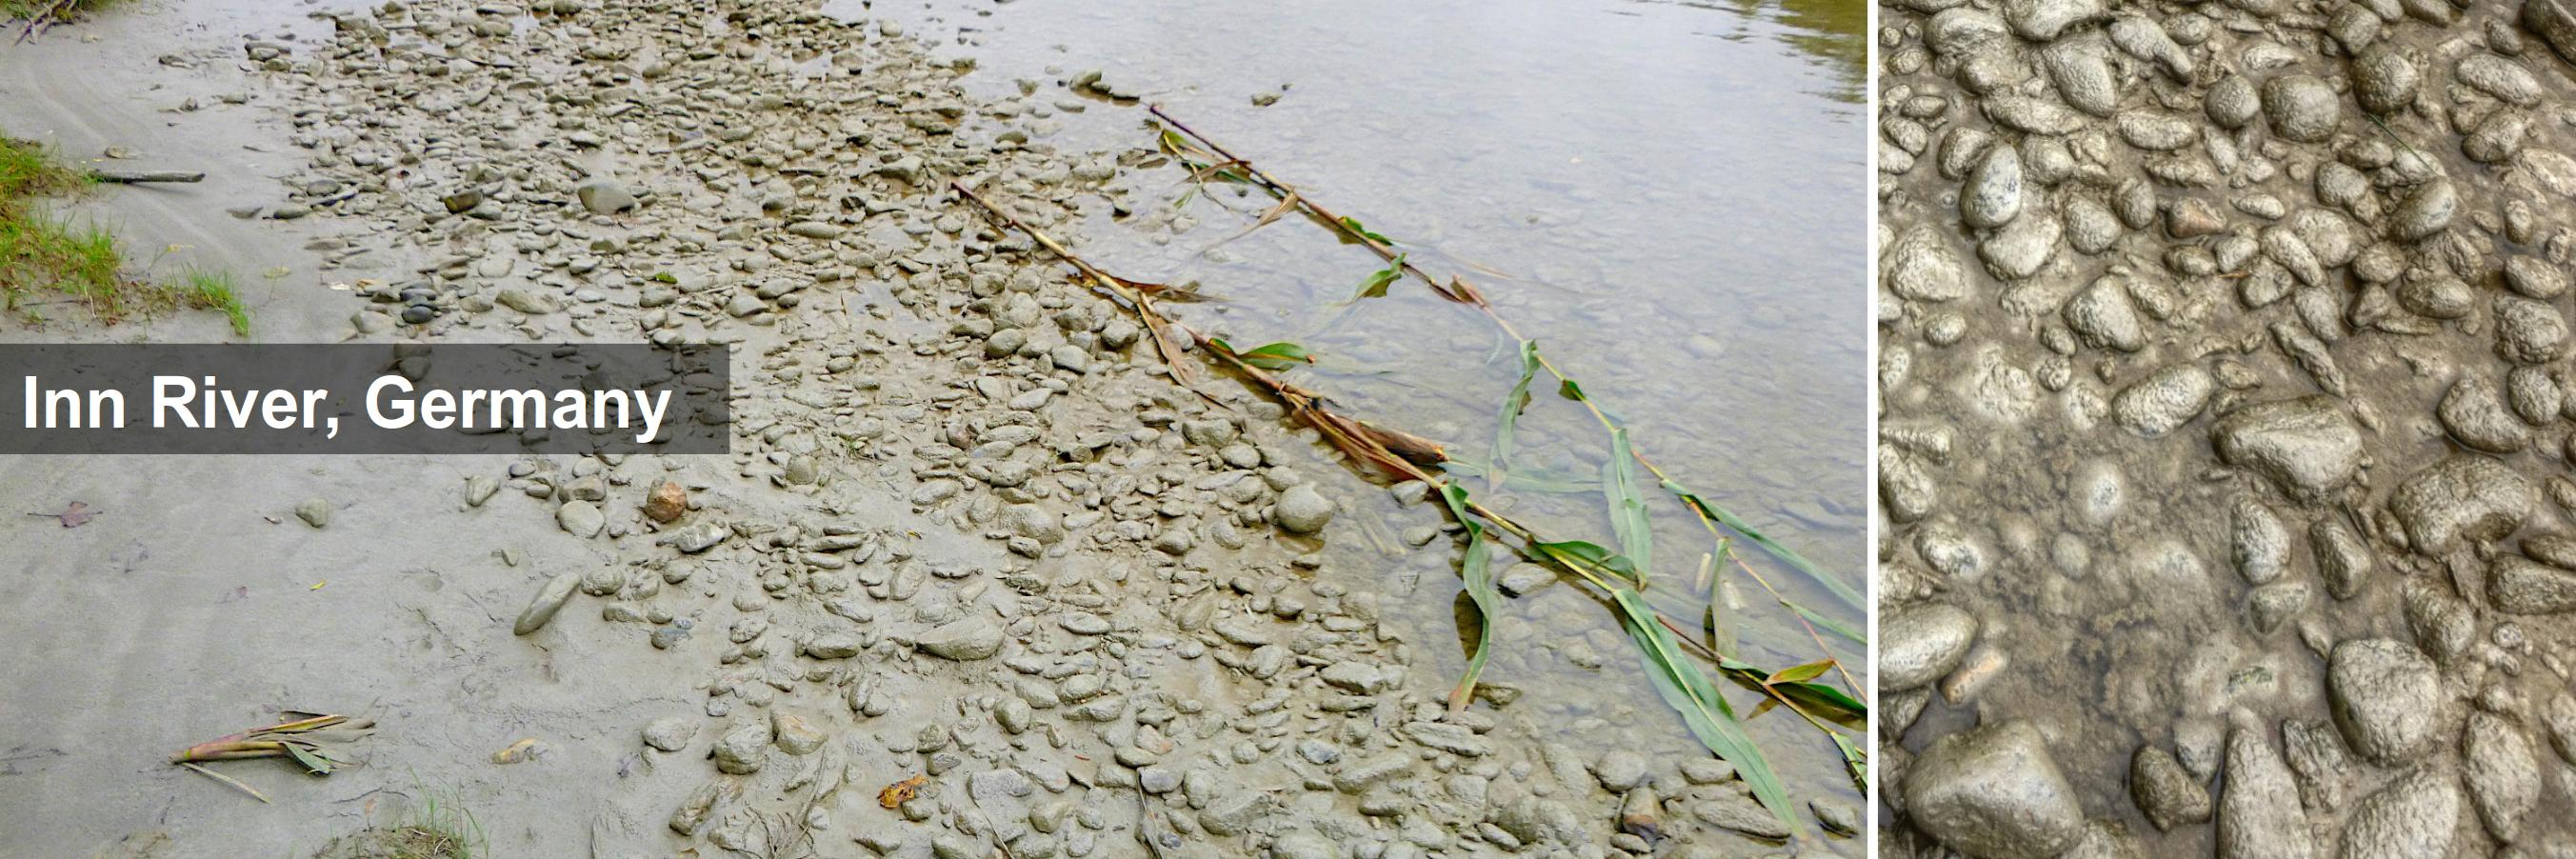
\includegraphics[width=0.91\paperwidth]{inn-clogging}};
		\end{scope}}
		\onslide<2-2>{
		\begin{scope}
			\node[anchor=south west, xshift=0.0\paperwidth, yshift=0.3\paperheight] {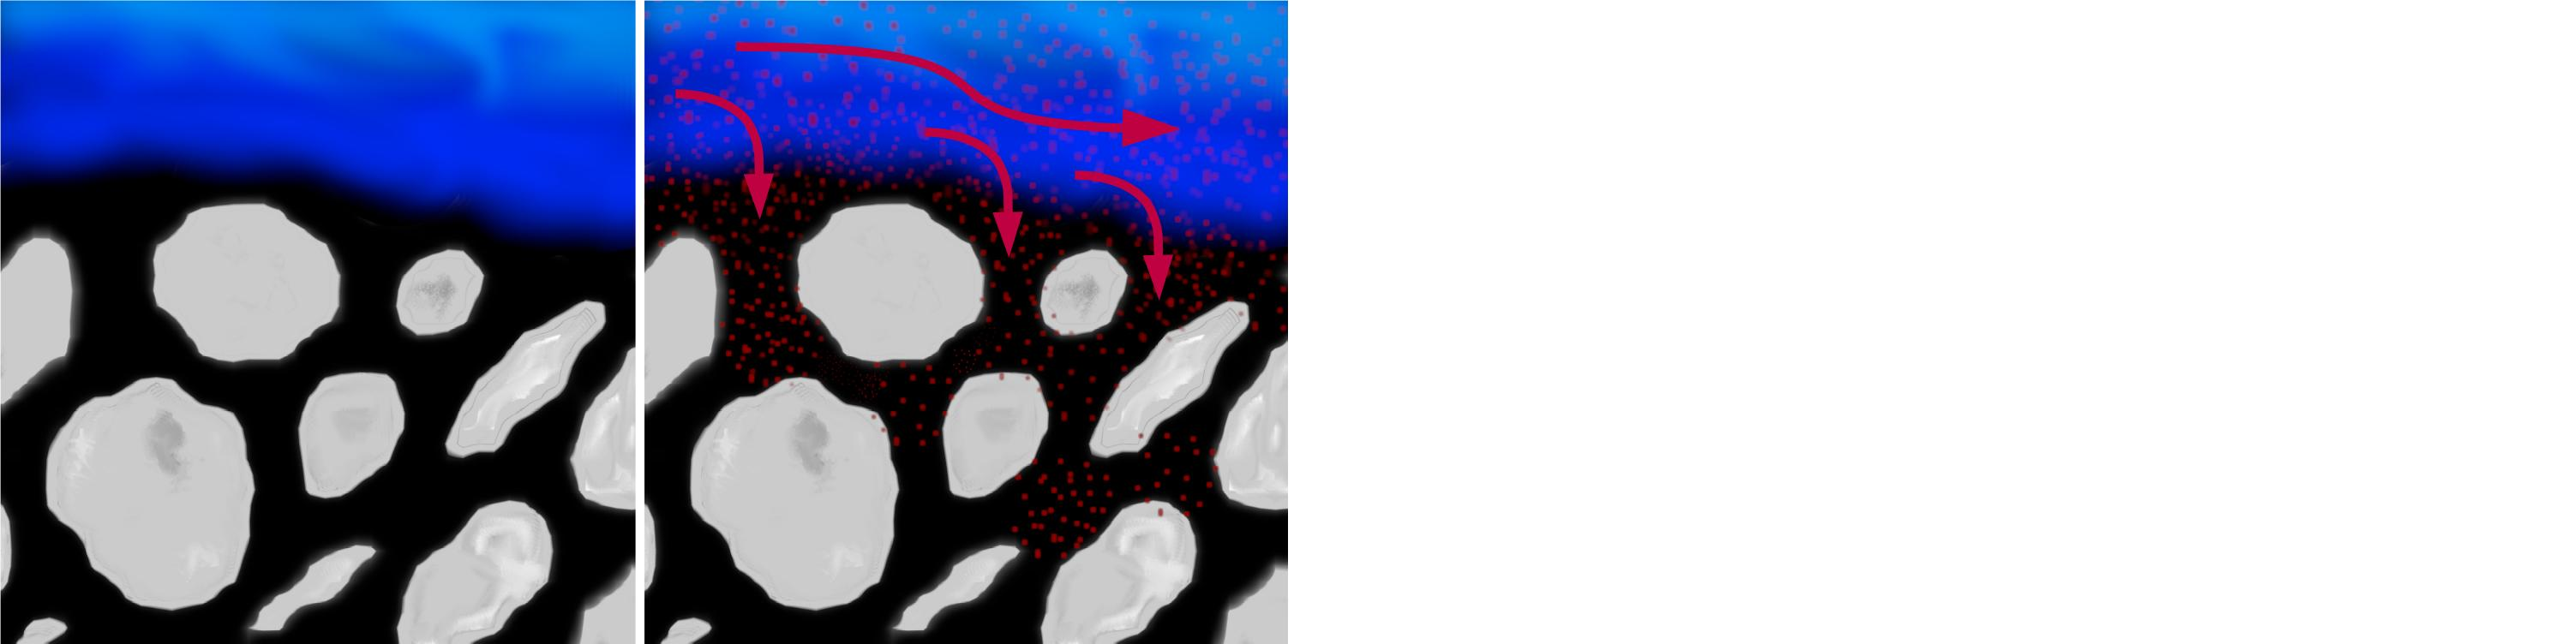
\includegraphics[width=0.91\paperwidth]{new-clogging-assembley-0}};
		\end{scope}}
		\onslide<3->{
			\begin{scope}
				\node[anchor=south west, xshift=0.0\paperwidth, yshift=0.3\paperheight] {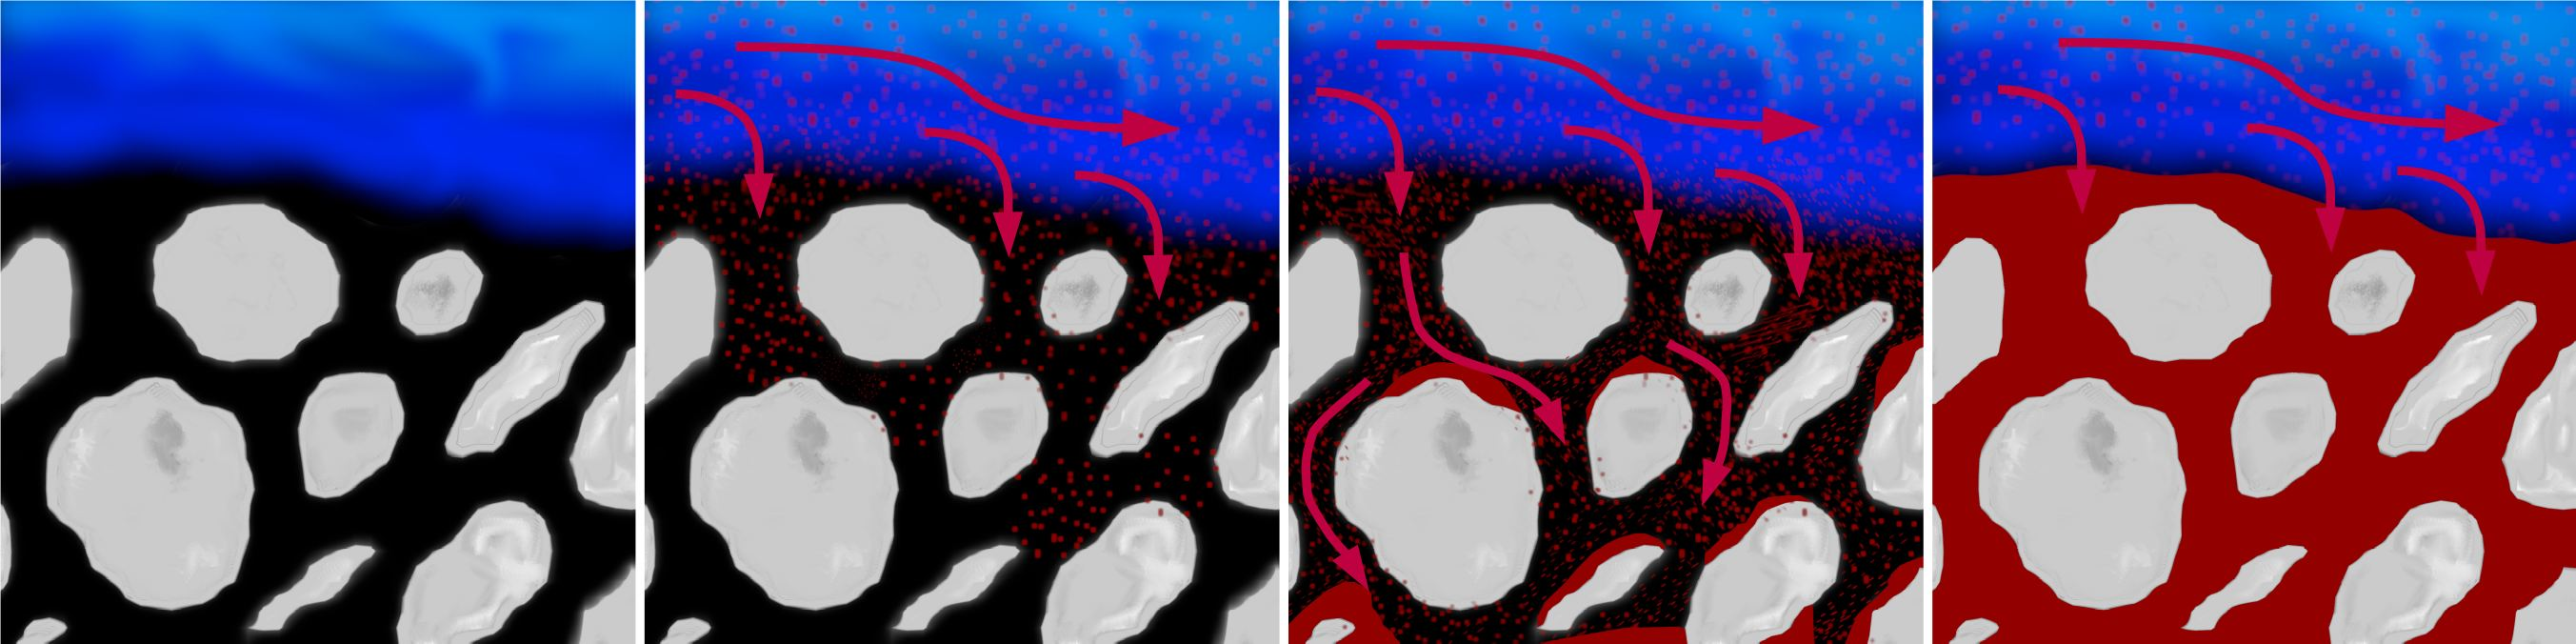
\includegraphics[width=0.91\paperwidth]{new-clogging-assembley-1}};
		\end{scope}}
		\onslide<2->{
		\node[anchor=south west, xshift=0.33\paperwidth, yshift=0.225\paperheight, text=black, text width=0.5\paperwidth,align=left]{\tiny Image concept adapted from \sscURL{Schälchli (1993)}{https://ethz.ch/content/dam/ethz/special-interest/baug/vaw/vaw-dam/documents/das-institut/mitteilungen/1990-1999/124.pdf}};}
	\end{tikzpicture}
\end{frame}

\subsection{Riverbed Clogging Measurement Methods}

\begin{frame}{\secname\vspace{0.1cm}\\\textcolor{anthrazit!80!white}{\subsecname}}\vspace{-0.8cm}
	\begin{columns}[T]
		\begin{column}{.5\textwidth}
			\sscFig{multipac}{The Multi-Parameter Approach for
				assessing riverbed Clogging (MultiPAC -- \sscURL{Negreiros \textit{et al.}, 2023}{https://onlinelibrary.wiley.com/doi/abs/10.1002/rra.4145}; \sscURL{Seitz, 2020}{http://dx.doi.org/10.18419/opus-11249}. Imagery: \sscURL{Schwindt \textit{et al.}, 2023}{https://www.sciencedirect.com/science/article/pii/S1470160X23011871})}
		\end{column}\hspace{-0.5cm}
		\begin{column}{.4313\textwidth}\vspace{0.77cm}
			\onslide<1->{
				\sscFig{sfm-freeze-core-19}{MultiPAC measurements at the Inn}\vspace{-0.5cm}
			}
			\onslide<2->{
				\faHandORight\ \textbf{Grain sizes, porosity, interstitial dissolved oxygen concentration (IDOC), hydraulic conductivity}}
		\end{column}
	\end{columns}
	% \textbf{Water temperature, filter velocity (for hydraulic conductivity), pH value,\\\hspace{0.4cm} interstitial dissolved oxygen}}
\end{frame}

\subsection{Engineering Solutions to Reinstate Vertical Connectivity Locally}
\begin{frame}{\secname\vspace{0.1cm}\\\textcolor{anthrazit!80!white}{\subsecname}}
	\begin{tikzpicture}
		\clip (0,0) rectangle (\paperwidth,\paperheight);
		\onslide<1->{
		\begin{scope}
				\node[anchor=south west, xshift=0.0\paperwidth, yshift=0.295\paperheight] {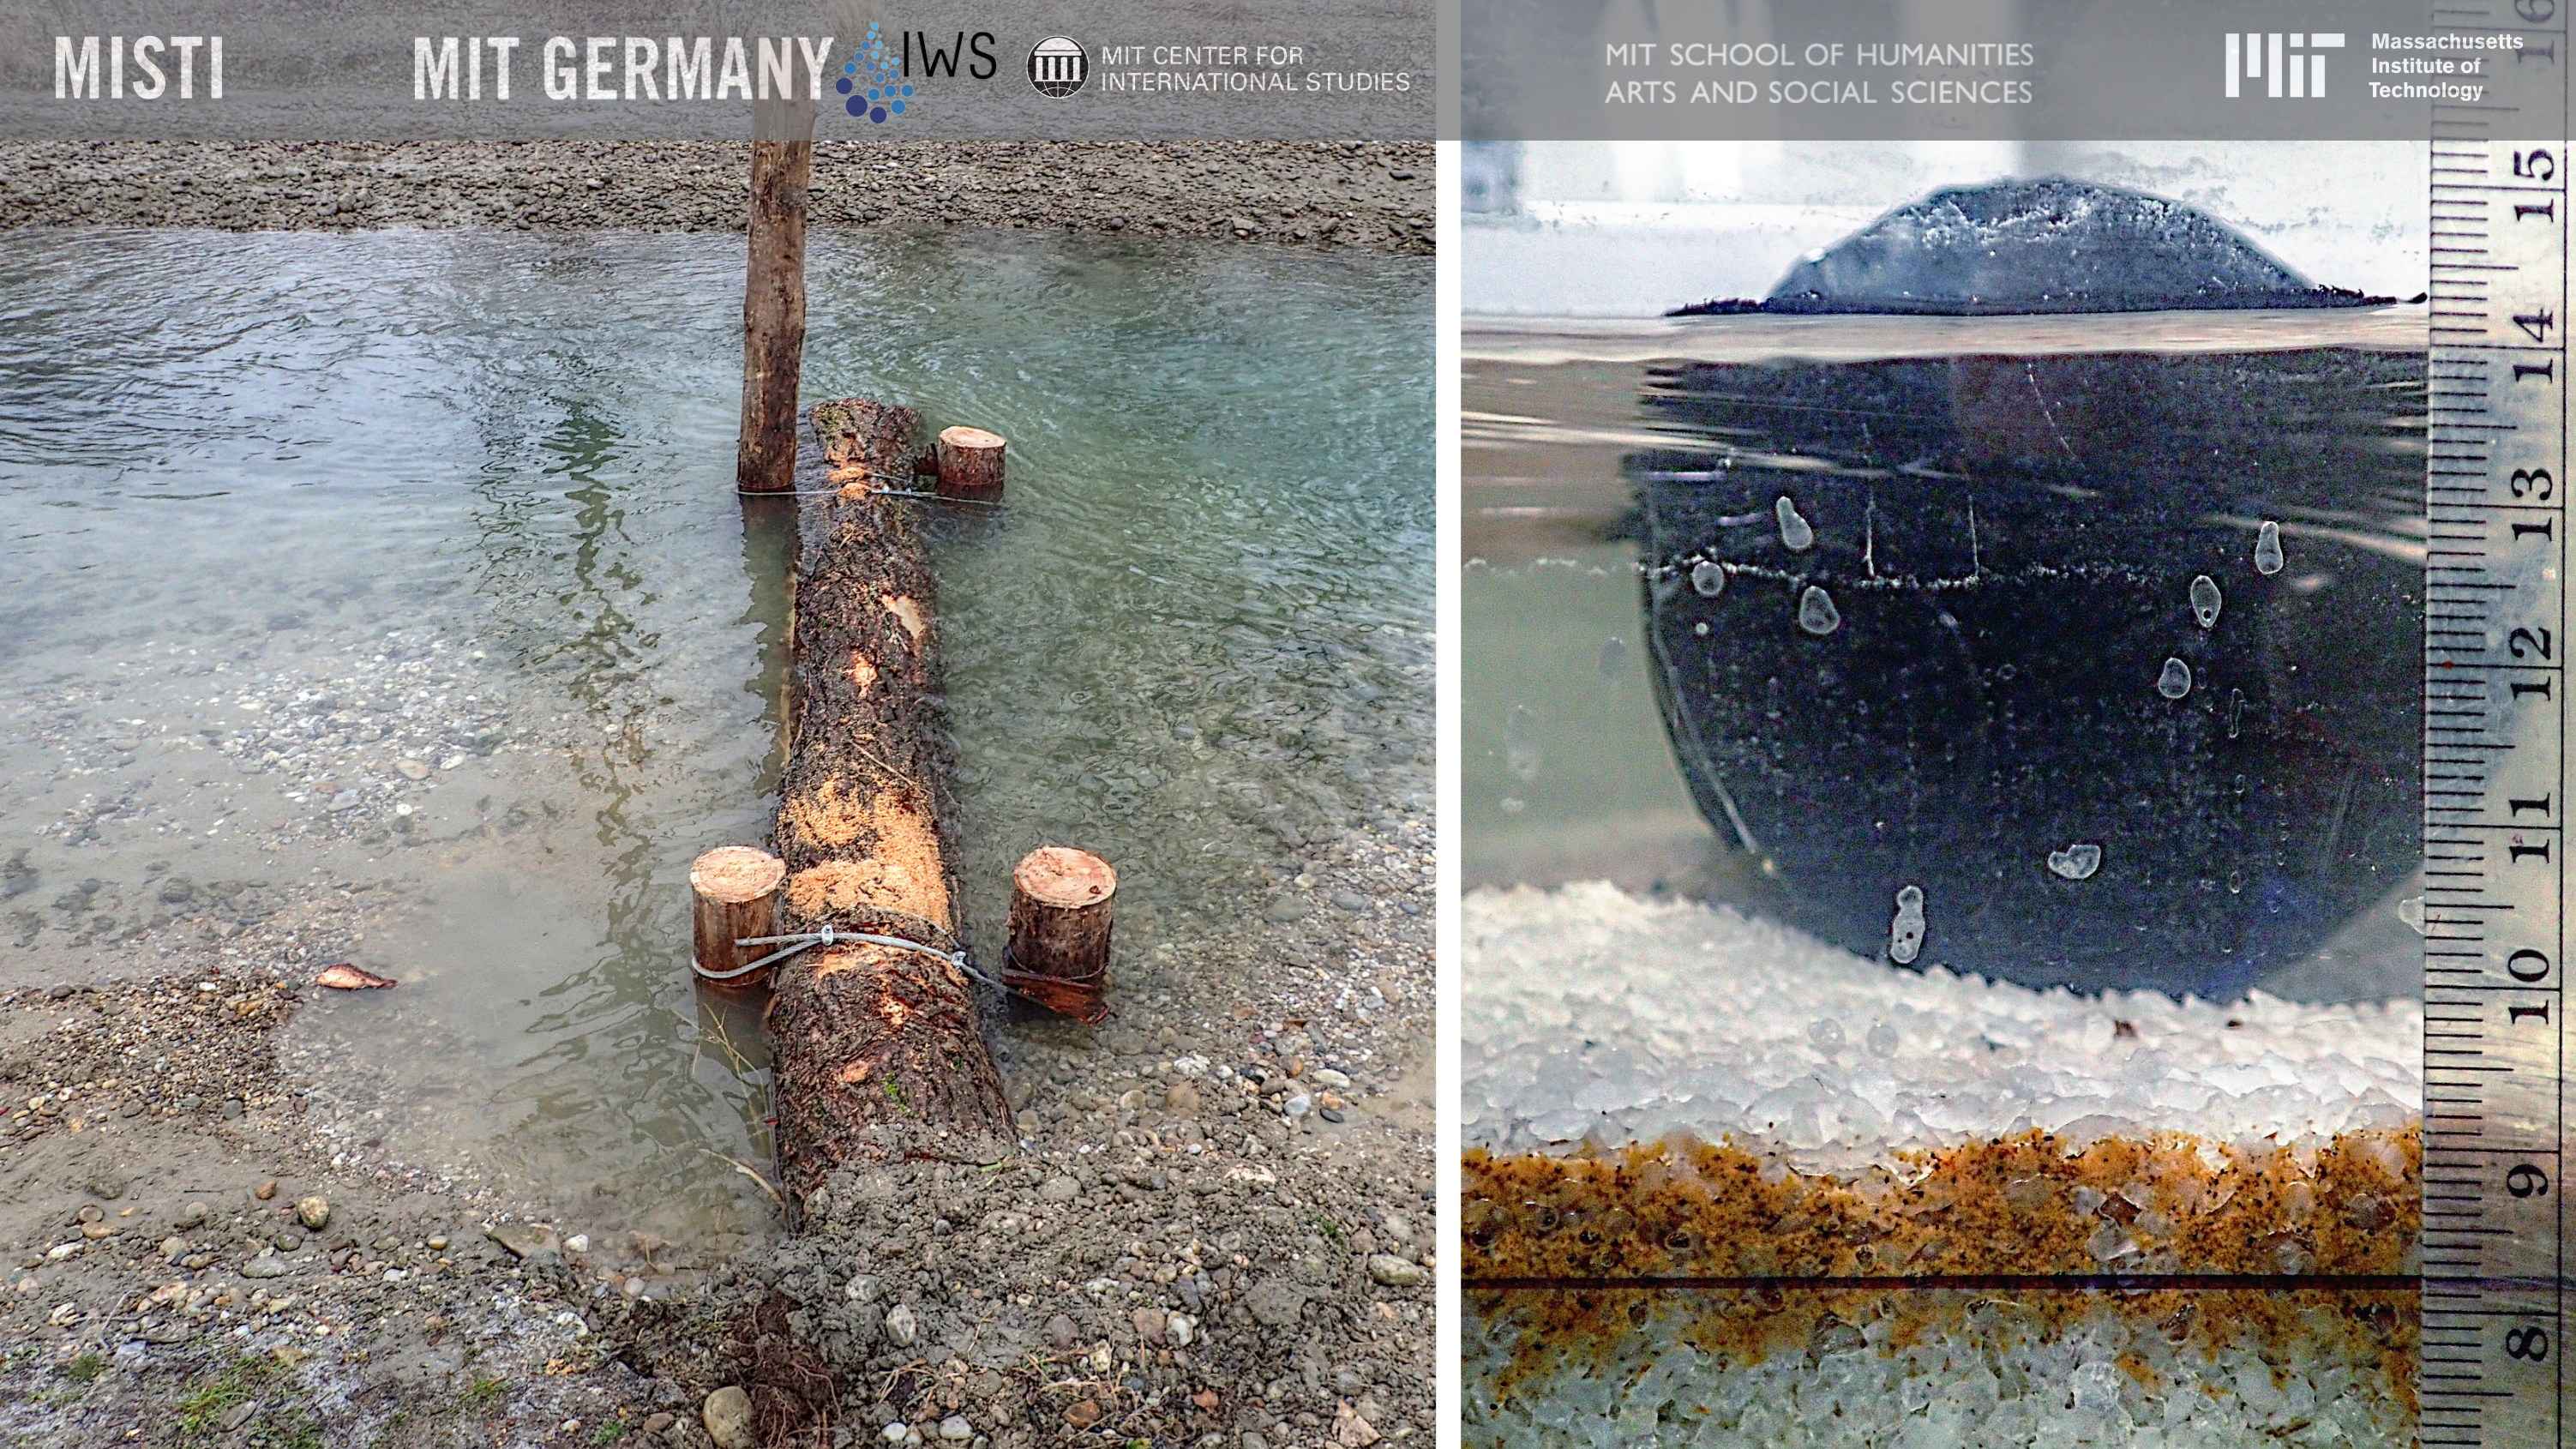
\includegraphics[width=0.86\paperwidth]{lwm-experiment}};
		\end{scope}}
	%	\onslide<1->{
	%		\node[anchor=south west, xshift=0.33\paperwidth, yshift=0.225\paperheight, text=black, text width=0.5\paperwidth,align=left]{\tiny Images adapted from Schwindt \textit{et al.} (2023, subm.)};}
	\end{tikzpicture}
\end{frame}


\begin{frame}{\secname\vspace{0.1cm}\\\textcolor{anthrazit!80!white}{\subsecname}}
	\begin{tikzpicture}
		\clip (0,0) rectangle (\paperwidth,\paperheight);
		\onslide<1->{
		\begin{scope}
				\node[anchor=south west, xshift=0.0\paperwidth, yshift=0.25\paperheight] {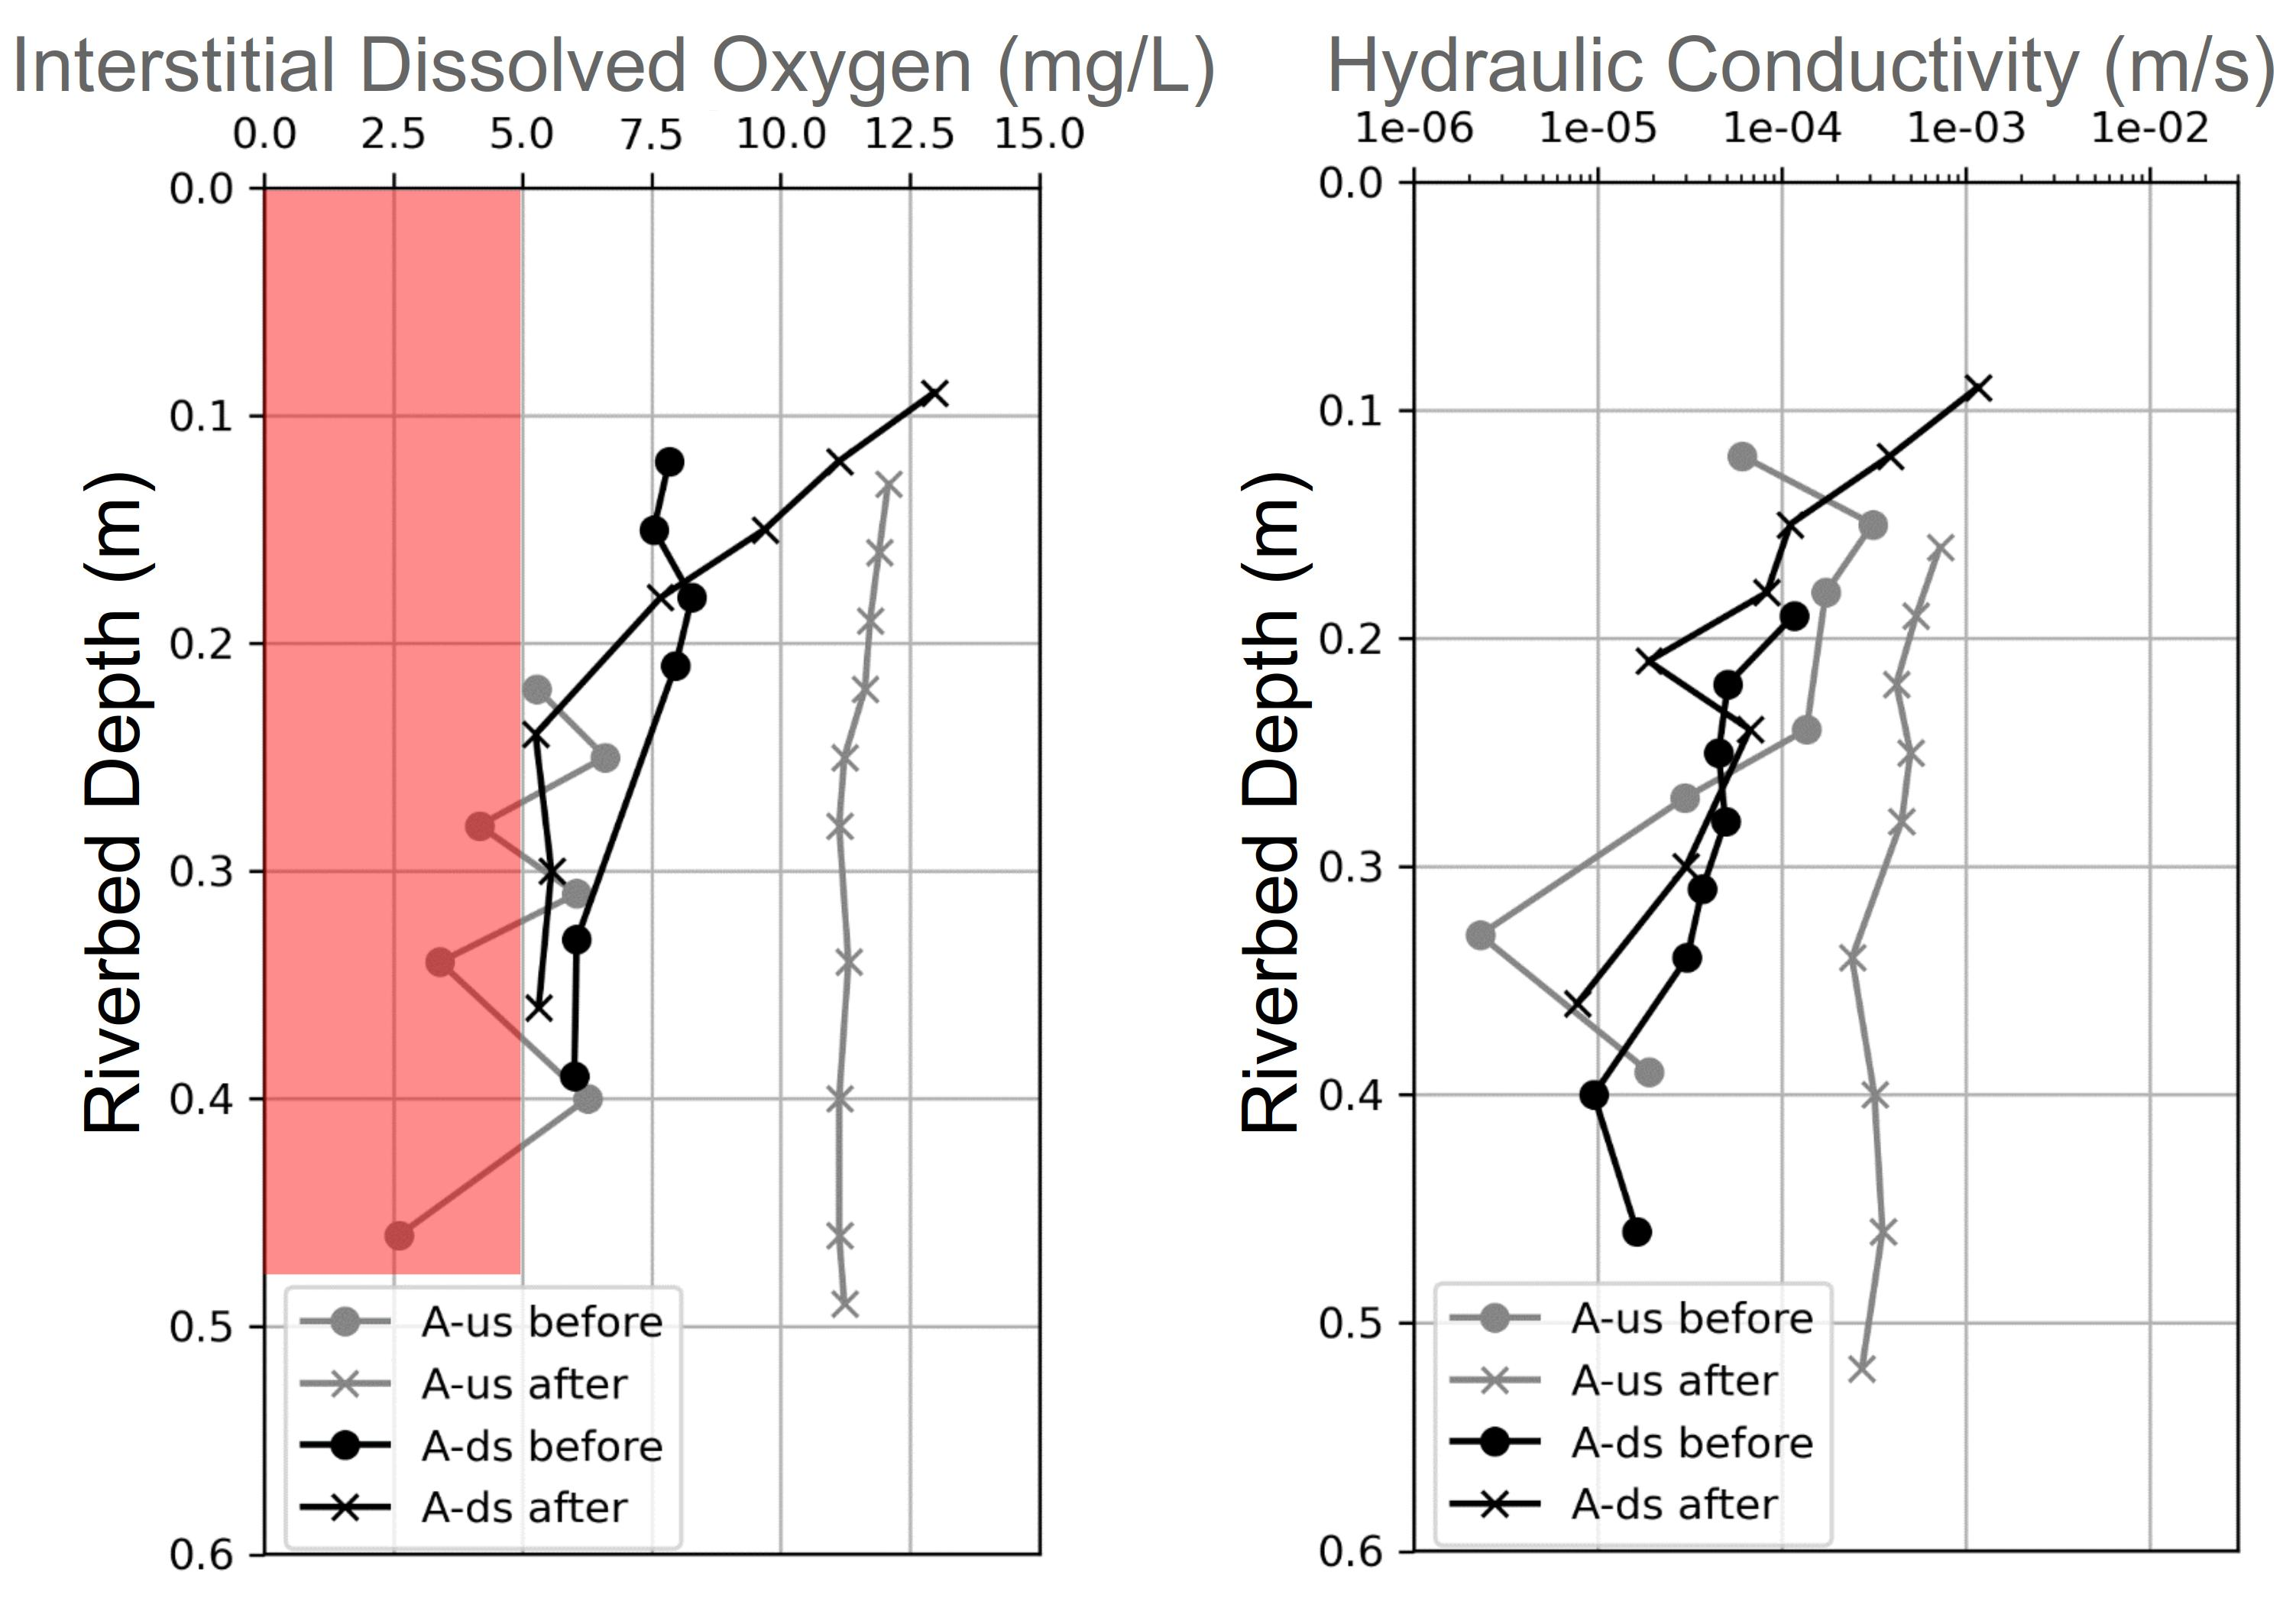
\includegraphics[width=0.8\paperwidth]{idoc-kf-results}};
		\end{scope}
		}
		\onslide<1->{
			\node[anchor=south west, xshift=0.33\paperwidth, yshift=0.225\paperheight, text=black, text width=0.5\paperwidth,align=left]{\tiny Images adapted from \sscURL{Schwindt \textit{et al.}, 2023}{https://www.sciencedirect.com/science/article/pii/S1470160X23011871}};
			}
	\end{tikzpicture}
\end{frame}

{
\usebackgroundtemplate{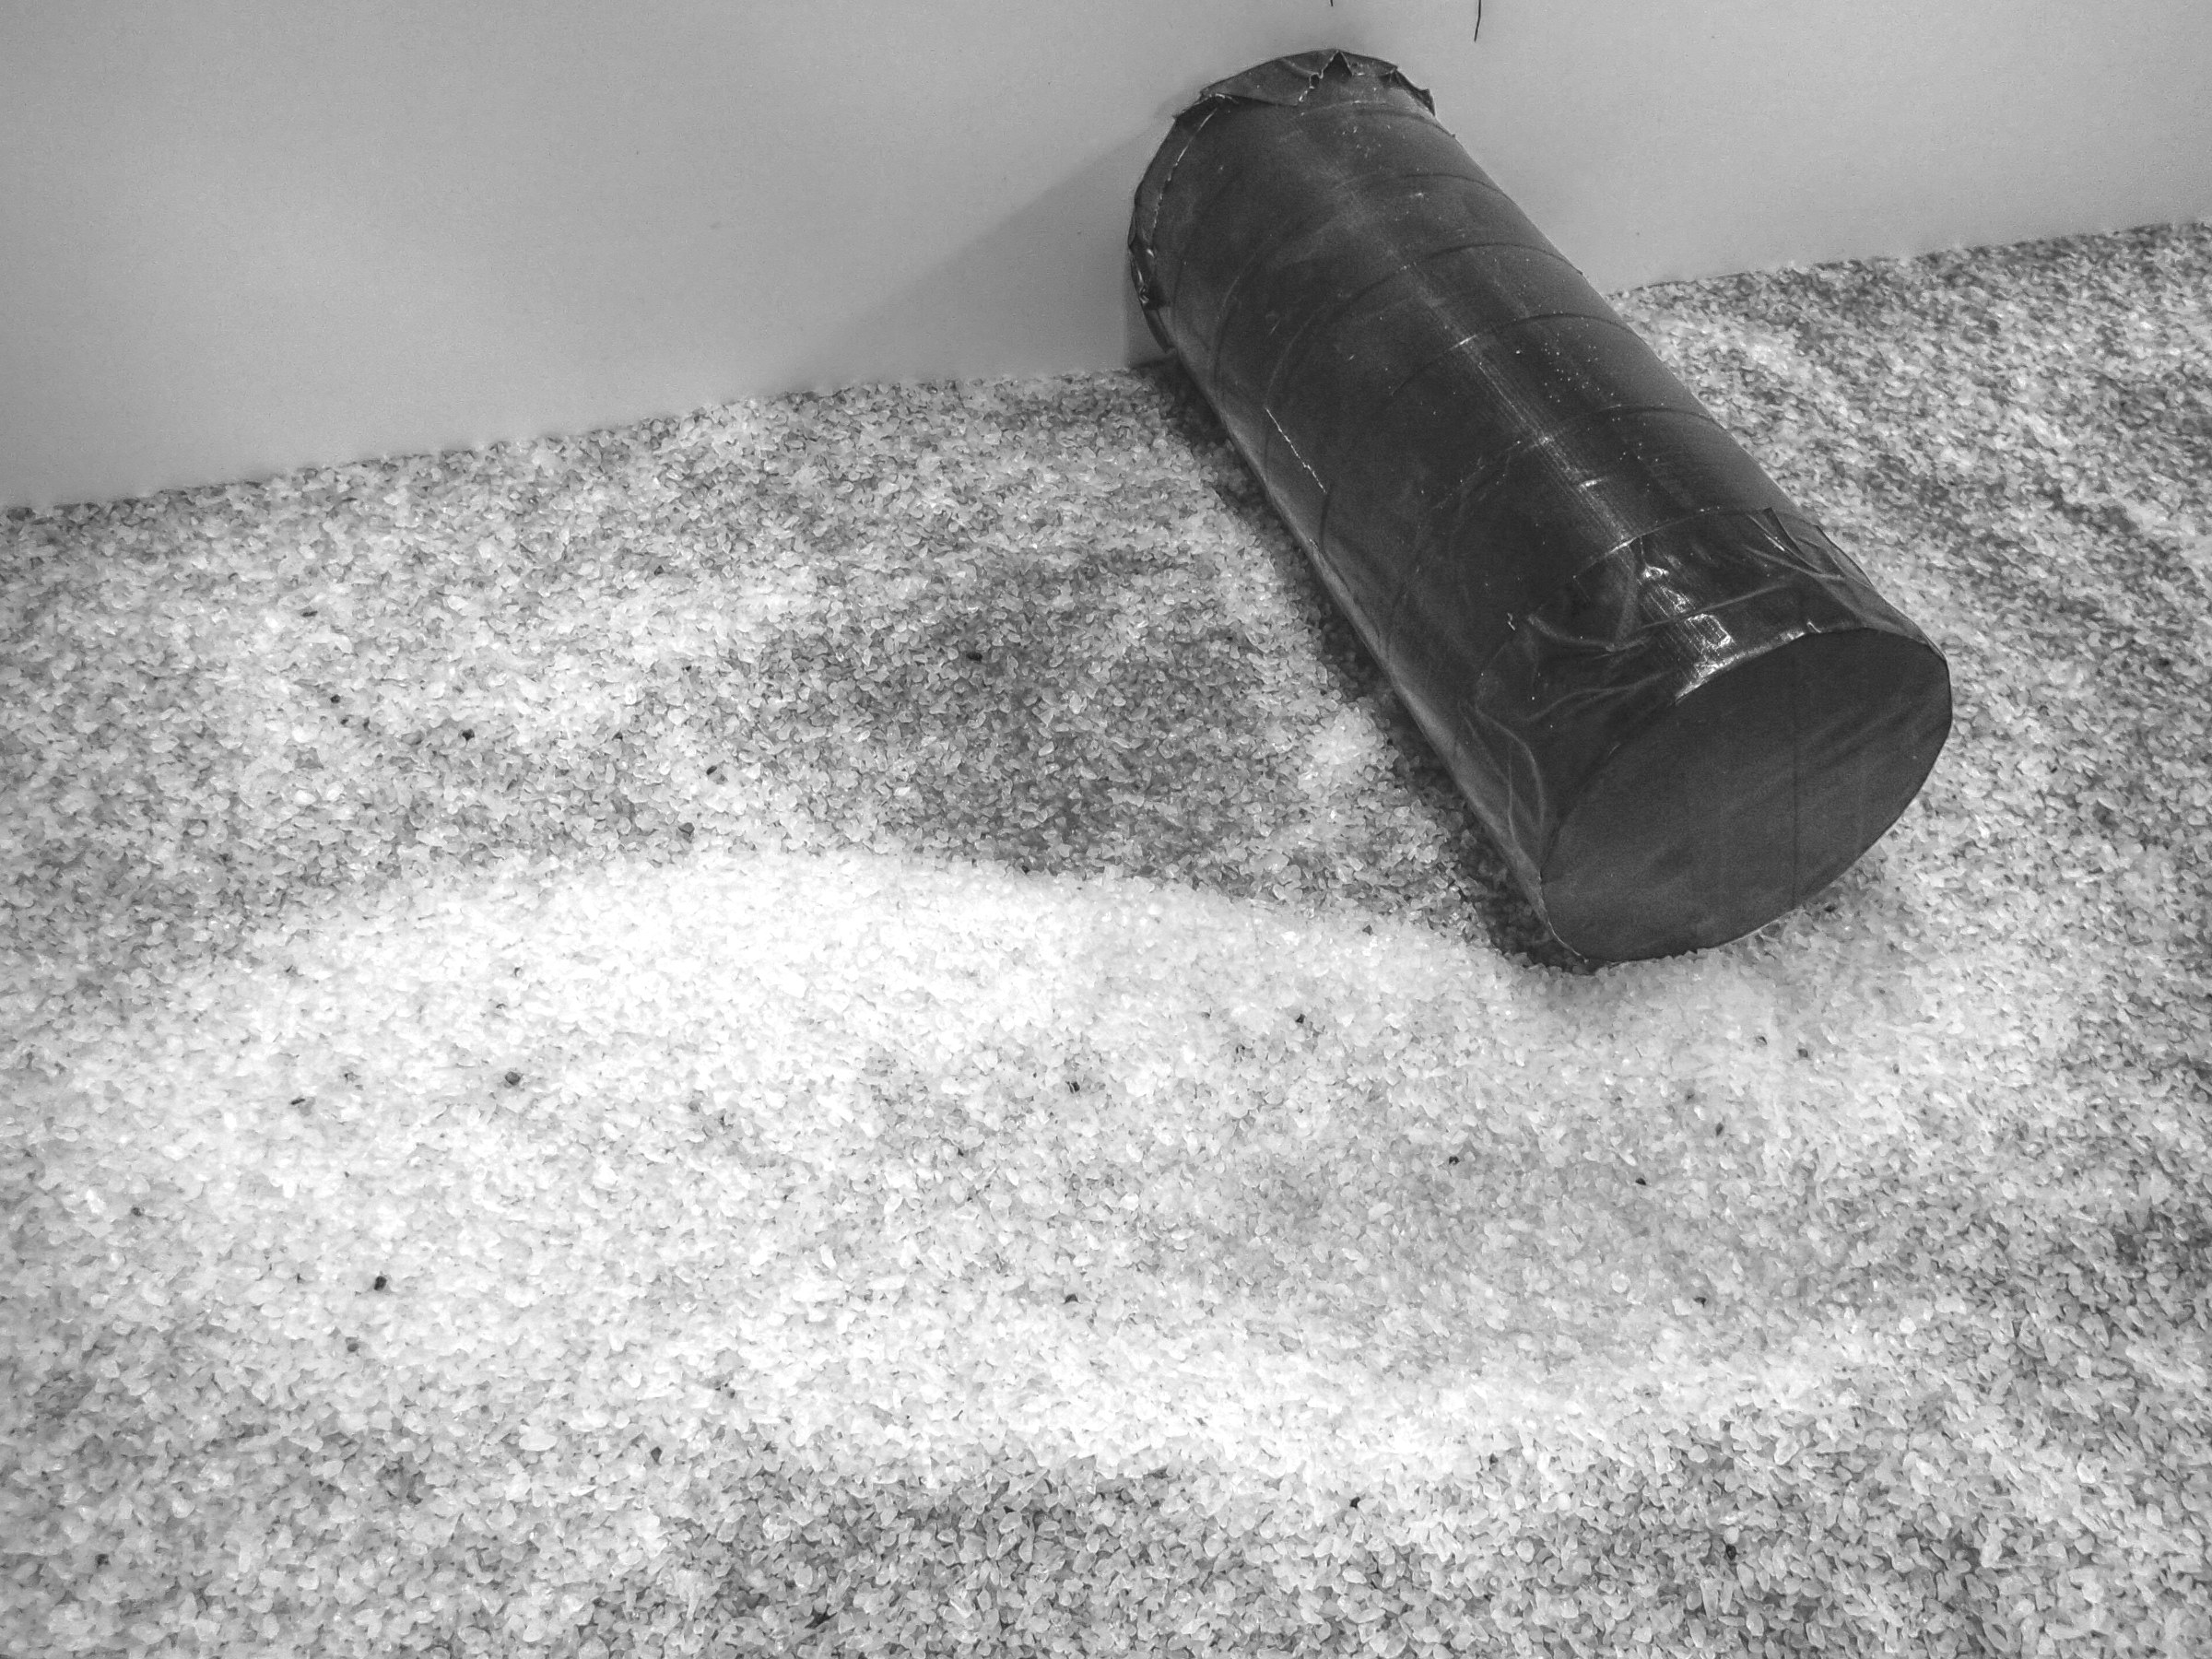
\includegraphics[width=\paperwidth]{test2-observations-18}}%
\begin{frame}[plain]{}{\secname}
	\vspace{3cm}
	\onslide<1->{
		\begin{tcolorbox}[colbacktitle=hellblau!80!black, colback=hellblau!10!white, fonttitle=\bfseries, standard jigsaw,colframe=blue_light, bottom=0mm, middle=0mm, boxsep=0.2mm, opacityframe=0.5, opacityfill=0.85, opacitybacktitle=0.95, title filled, title={Insights from the Nepf Lab}, size=fbox]
			\vspace{0.25cm}
			\begin{itemize}
				\item[\faChevronCircleRight]\ Emergent logs have higher declogging effect
				\item[\faChevronCircleRight]\ Elevated declogging in the wake of submerged logs
			\end{itemize}
			\vspace{0.25cm}
			{\small
				\begin{flushright}
				  \sscURL{Schalko/Ponce, Lassar, Schwindt, Haun, Nepf 2024}{https://www.nature.com/articles/s41598-023-47501-1}
				\end{flushright}
			}
		\end{tcolorbox}\smallskip}
\end{frame}}

%\begin{frame}{\secname\vspace{0.1cm}\\\textcolor{anthrazit!80!white}{\subsecname}}
%	\begin{tikzpicture}
%		\clip (0,0) rectangle (\paperwidth,\paperheight);
%			\begin{scope}
%				\begin{tcolorbox}[colbacktitle=hellblau!80!black, colback=hellblau!15!white, fonttitle=\bfseries, standard jigsaw,colframe=blue_light, bottom=0mm, middle=0mm, boxsep=0.2mm, opacityframe=0.5, opacityfill=0.75, opacitybacktitle=0.95, title filled, title={Insights from the Nepf Lab}, size=fbox]
%					\vspace{0.25cm}	 
%					\begin{itemize}
%						\item[\faChevronCircleRight]\ Emergent logs have higher declogging effect
%						\item[\faChevronCircleRight]\ Elevated declogging in the wake of submerged logs
%					\end{itemize}
%					\vspace{0.25cm}
%					{\tiny Images adapted from \sscURL{Schalko/Ponce \textit{et al.}, 2024}{https://www.nature.com/articles/s41598-023-47501-1}}
%				\end{tcolorbox}\smallskip
%			\end{scope}
%
%	\end{tikzpicture}
%\end{frame}


\subsection{Combined Vertical and Lateral Connectivity}
\begin{frame}{\secname\vspace{0.1cm}\\\textcolor{anthrazit!80!white}{\subsecname}}
	Reconnecting the y-axis: bank removal
	\begin{tikzpicture}
		\clip (0,0) rectangle (\paperwidth,\paperheight);
		\onslide<1->{
			\begin{scope}
				\node[anchor=south west, xshift=0.\paperwidth, yshift=0.295\paperheight] {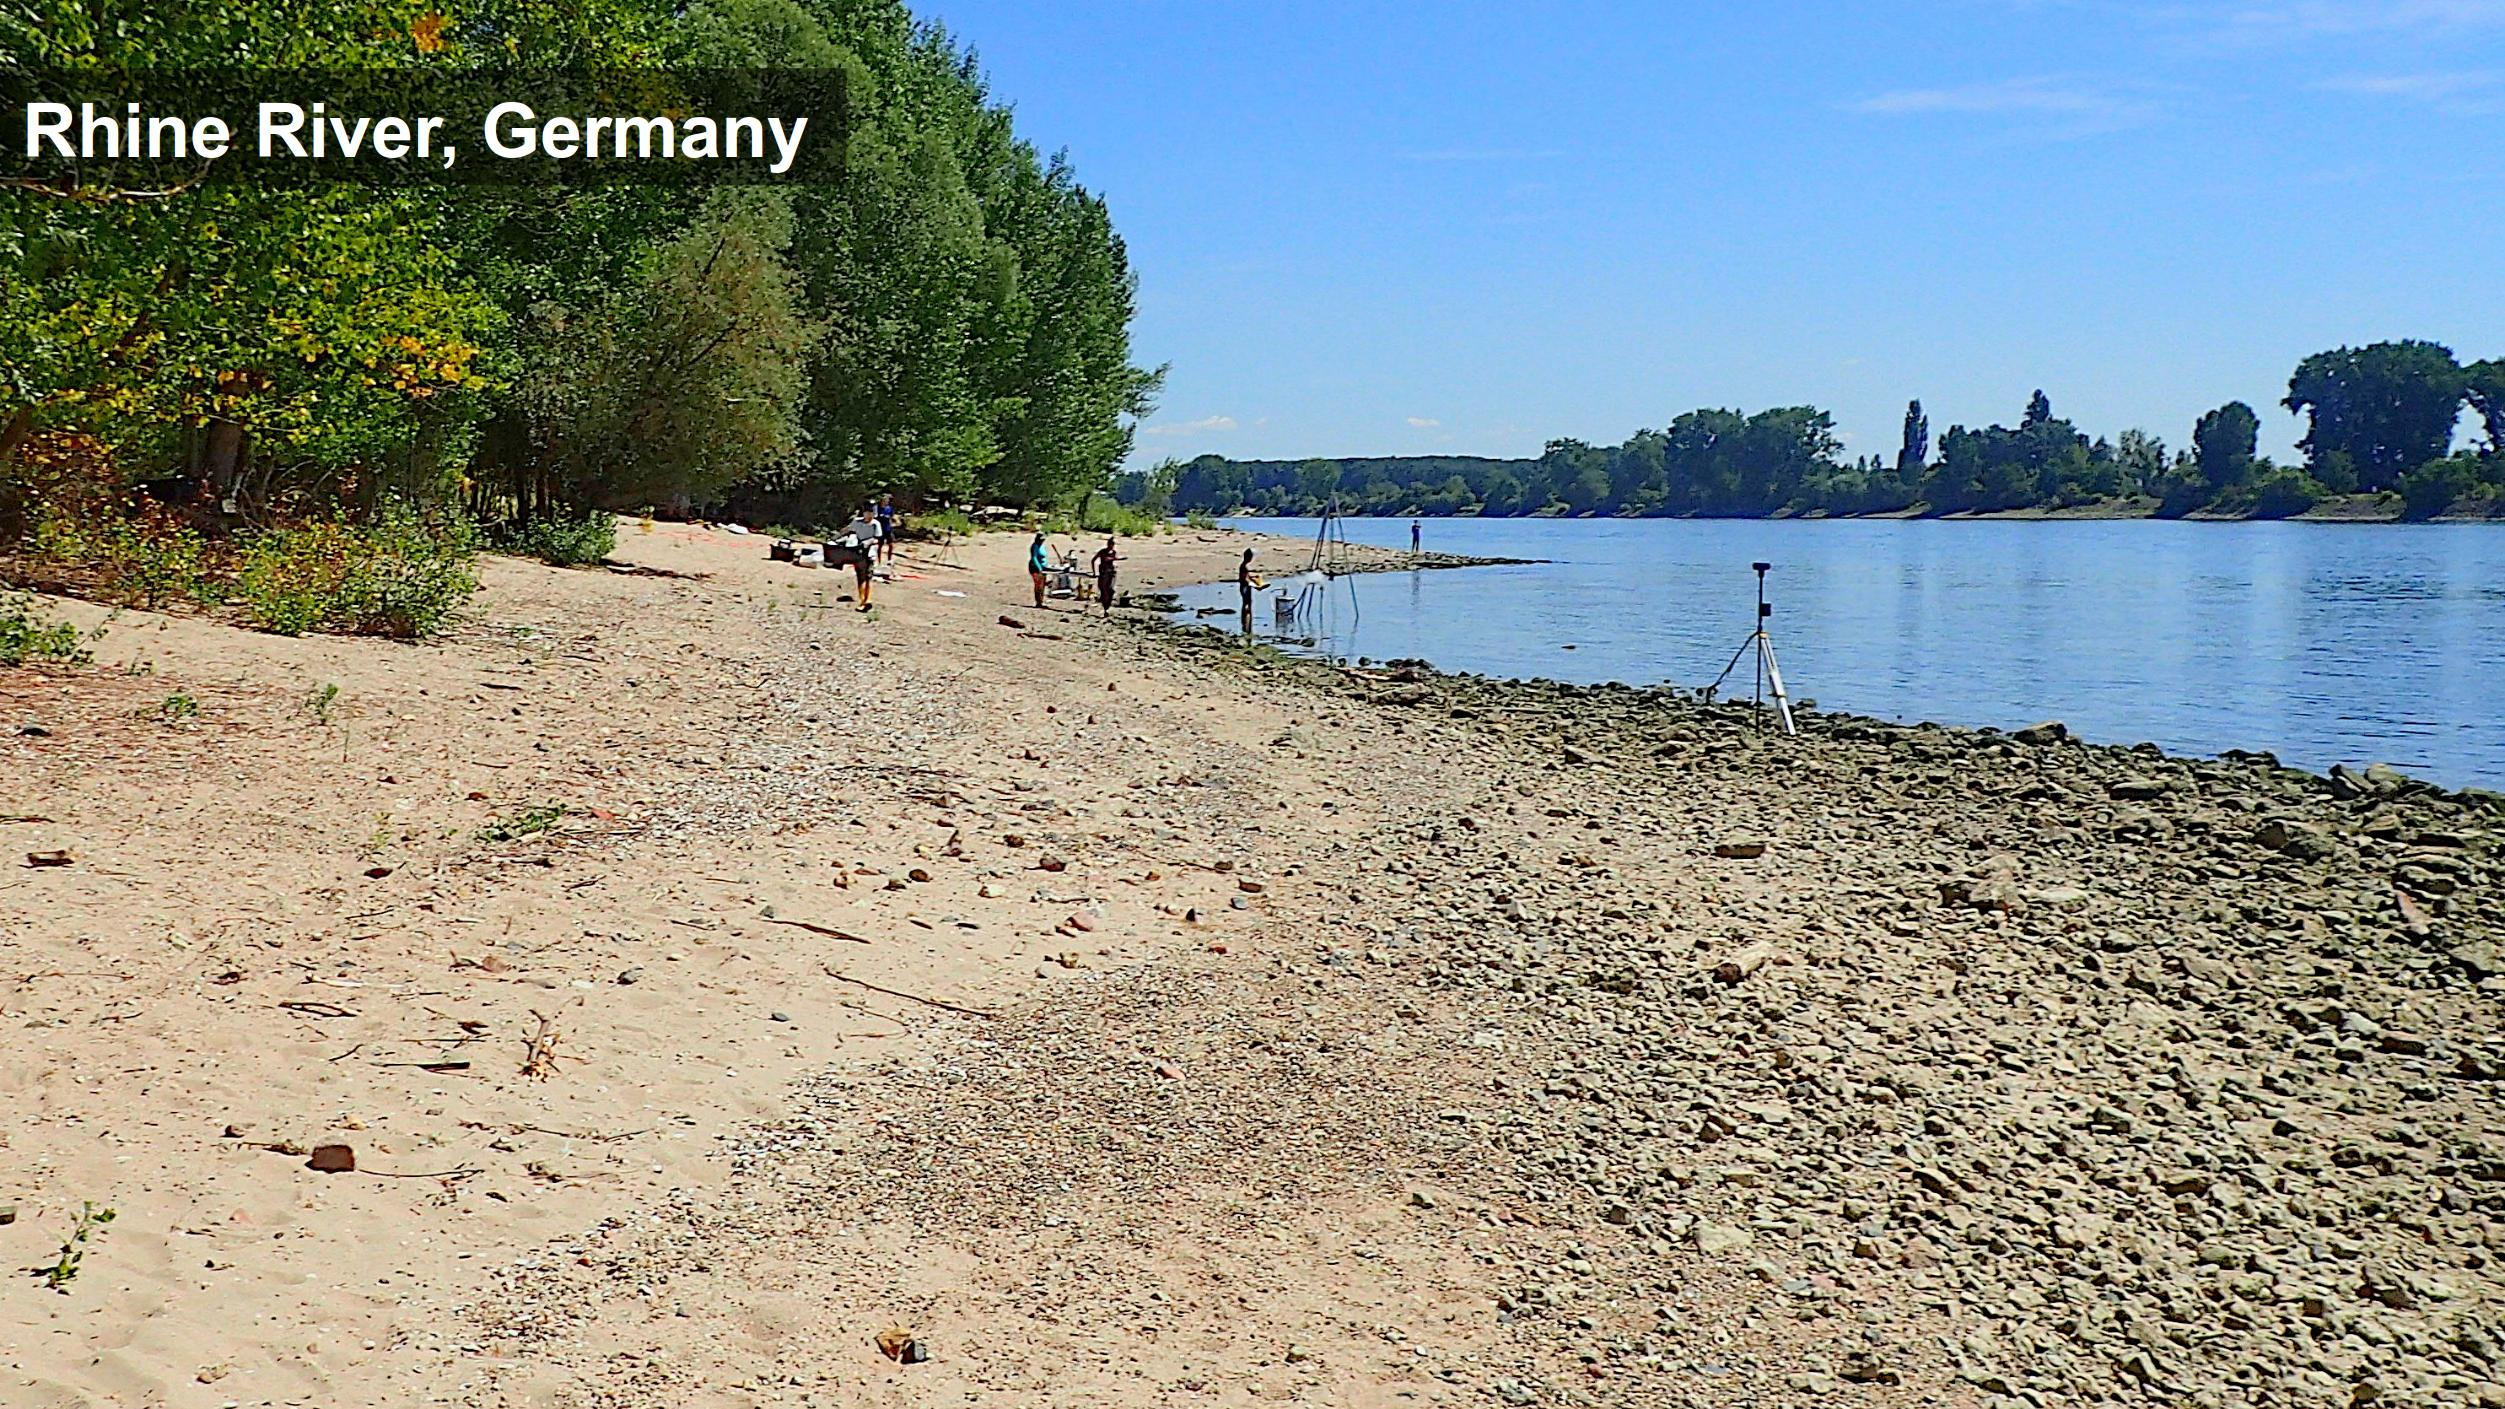
\includegraphics[width=0.86\paperwidth]{rhine-bank-removal-0}};
		\end{scope}}
		\onslide<2->{
			\begin{scope}
				\node[anchor=south west, xshift=0.\paperwidth, yshift=0.295\paperheight] {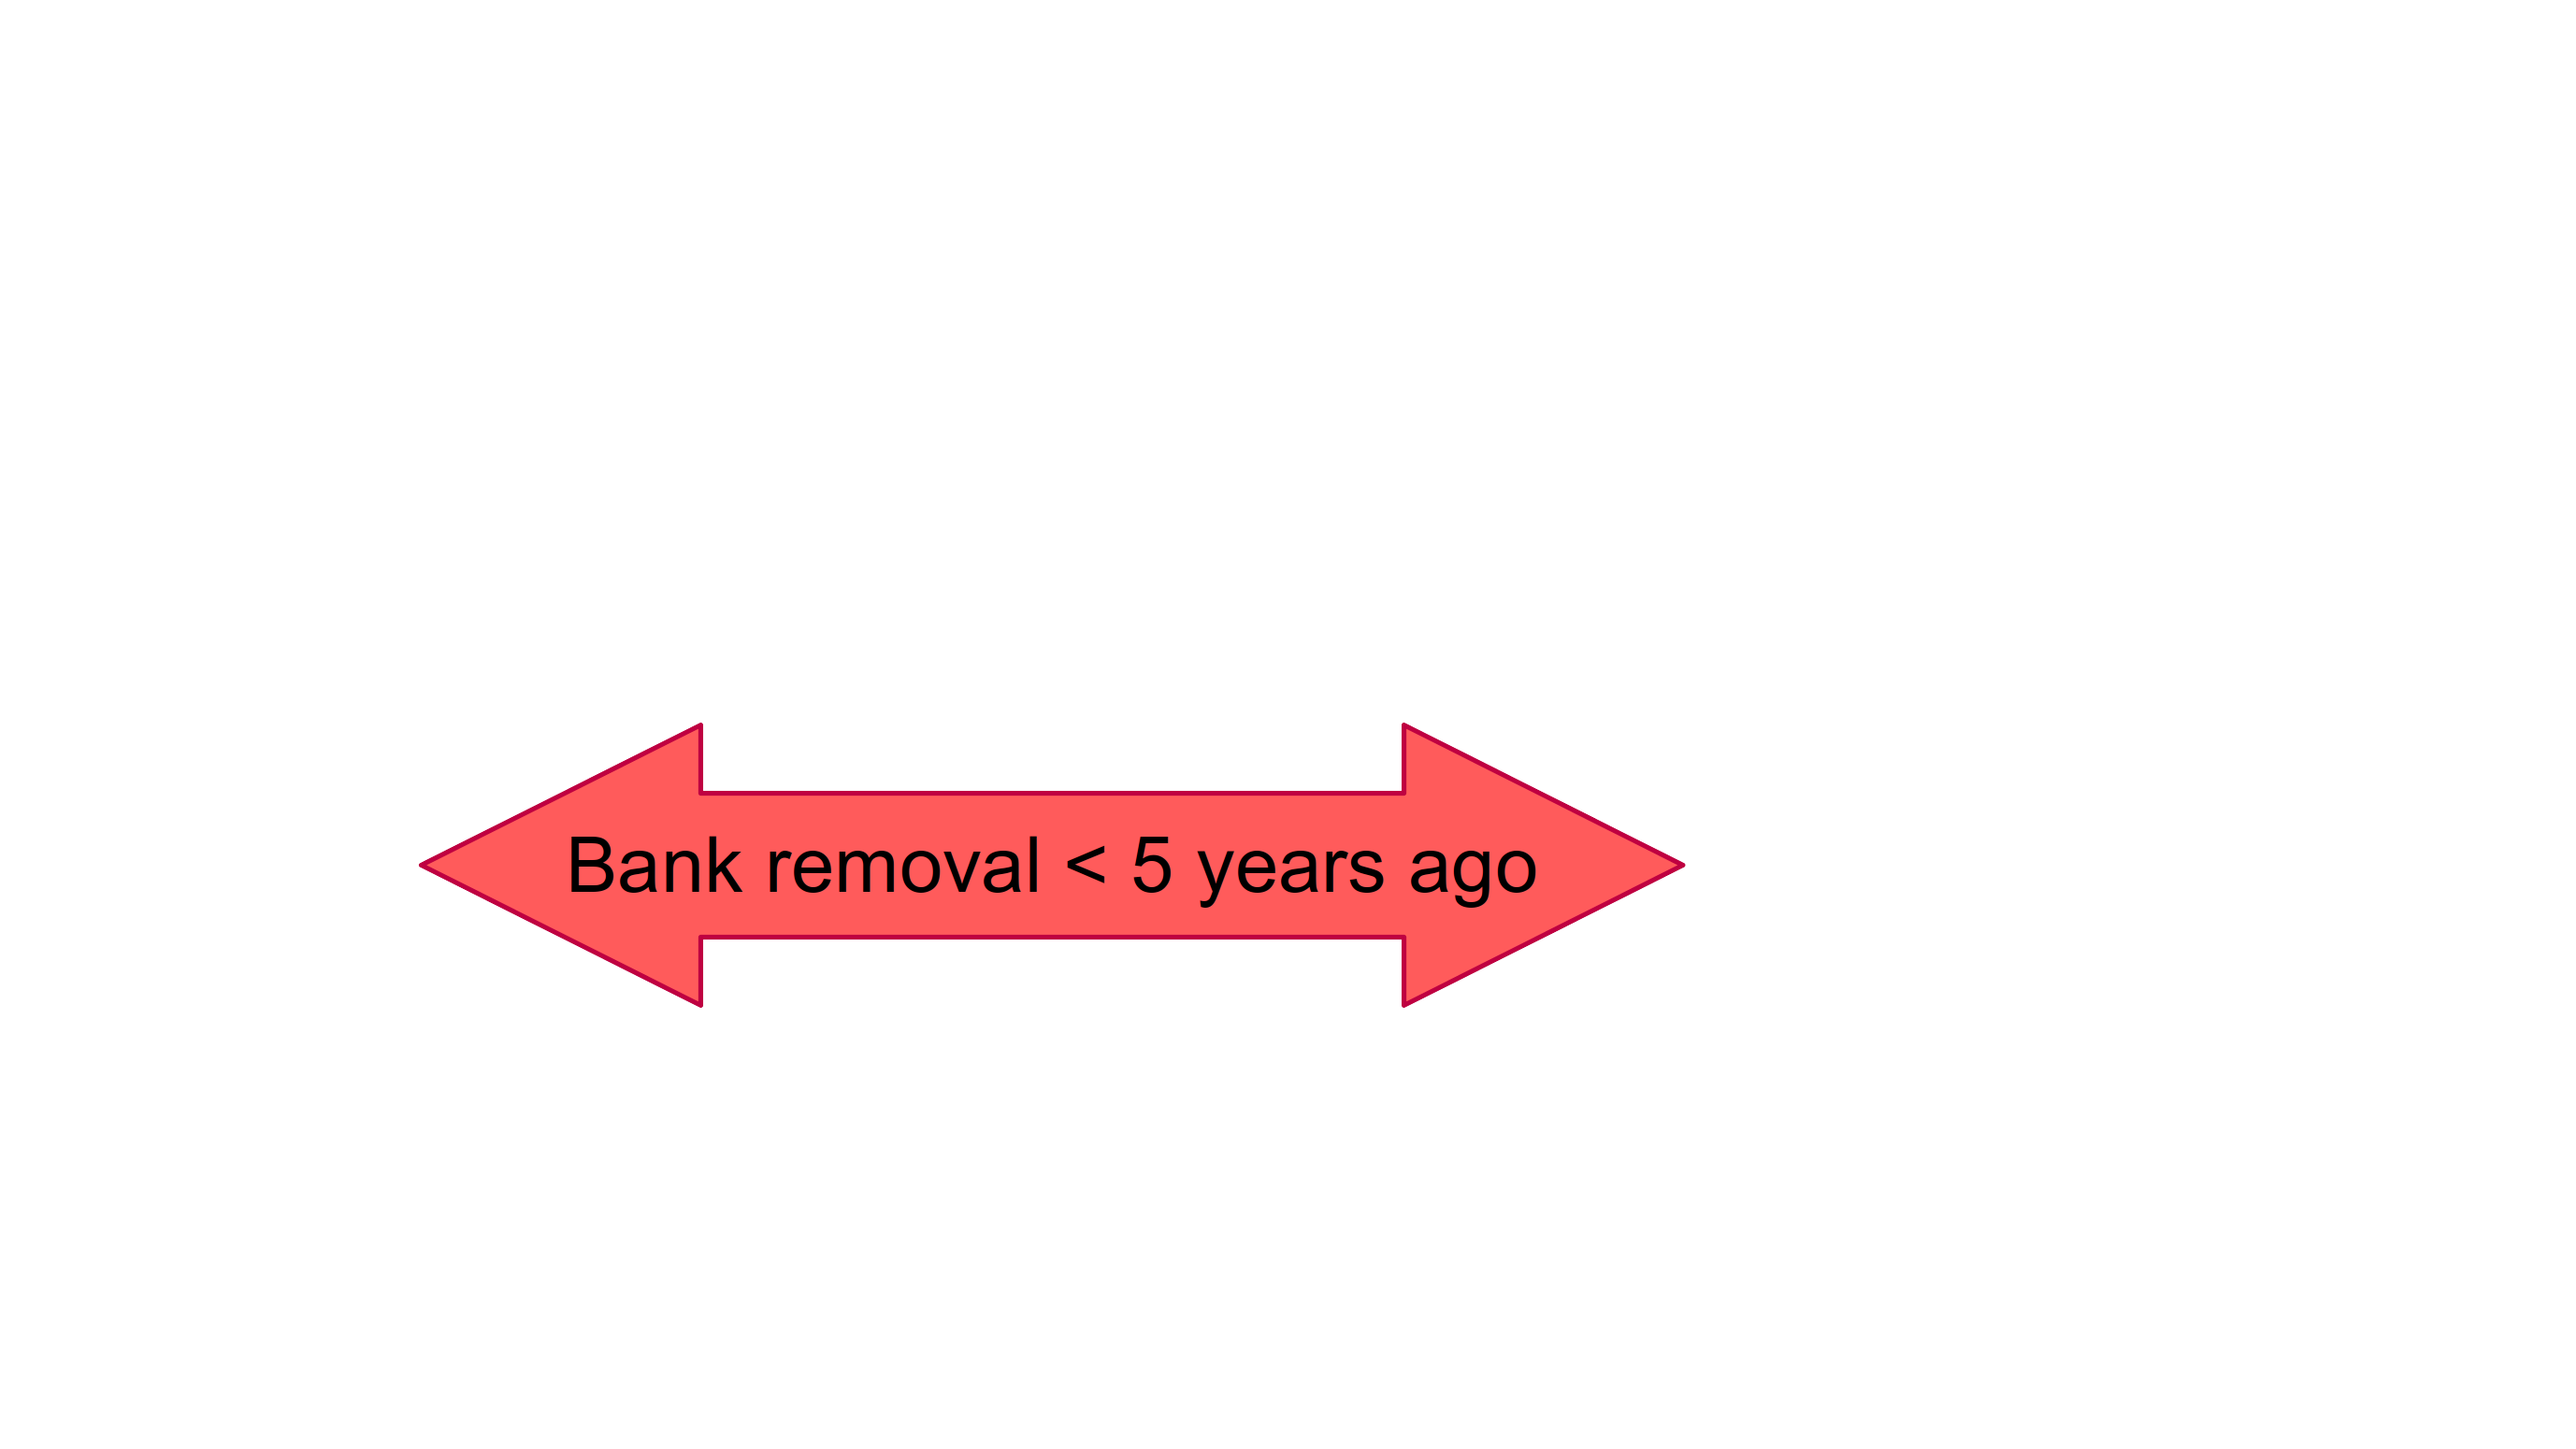
\includegraphics[width=0.86\paperwidth]{rhine-bank-removal-1}};
		\end{scope}}
	\end{tikzpicture}
\end{frame}

\begin{frame}{\secname\vspace{0.1cm}\\\textcolor{anthrazit!80!white}{\subsecname}}
	\begin{tikzpicture}
		\clip (0,0) rectangle (\paperwidth,\paperheight);
		\onslide<1->{
		\begin{scope}
			\node[anchor=south west, xshift=0.0\paperwidth, yshift=0.27\paperheight] {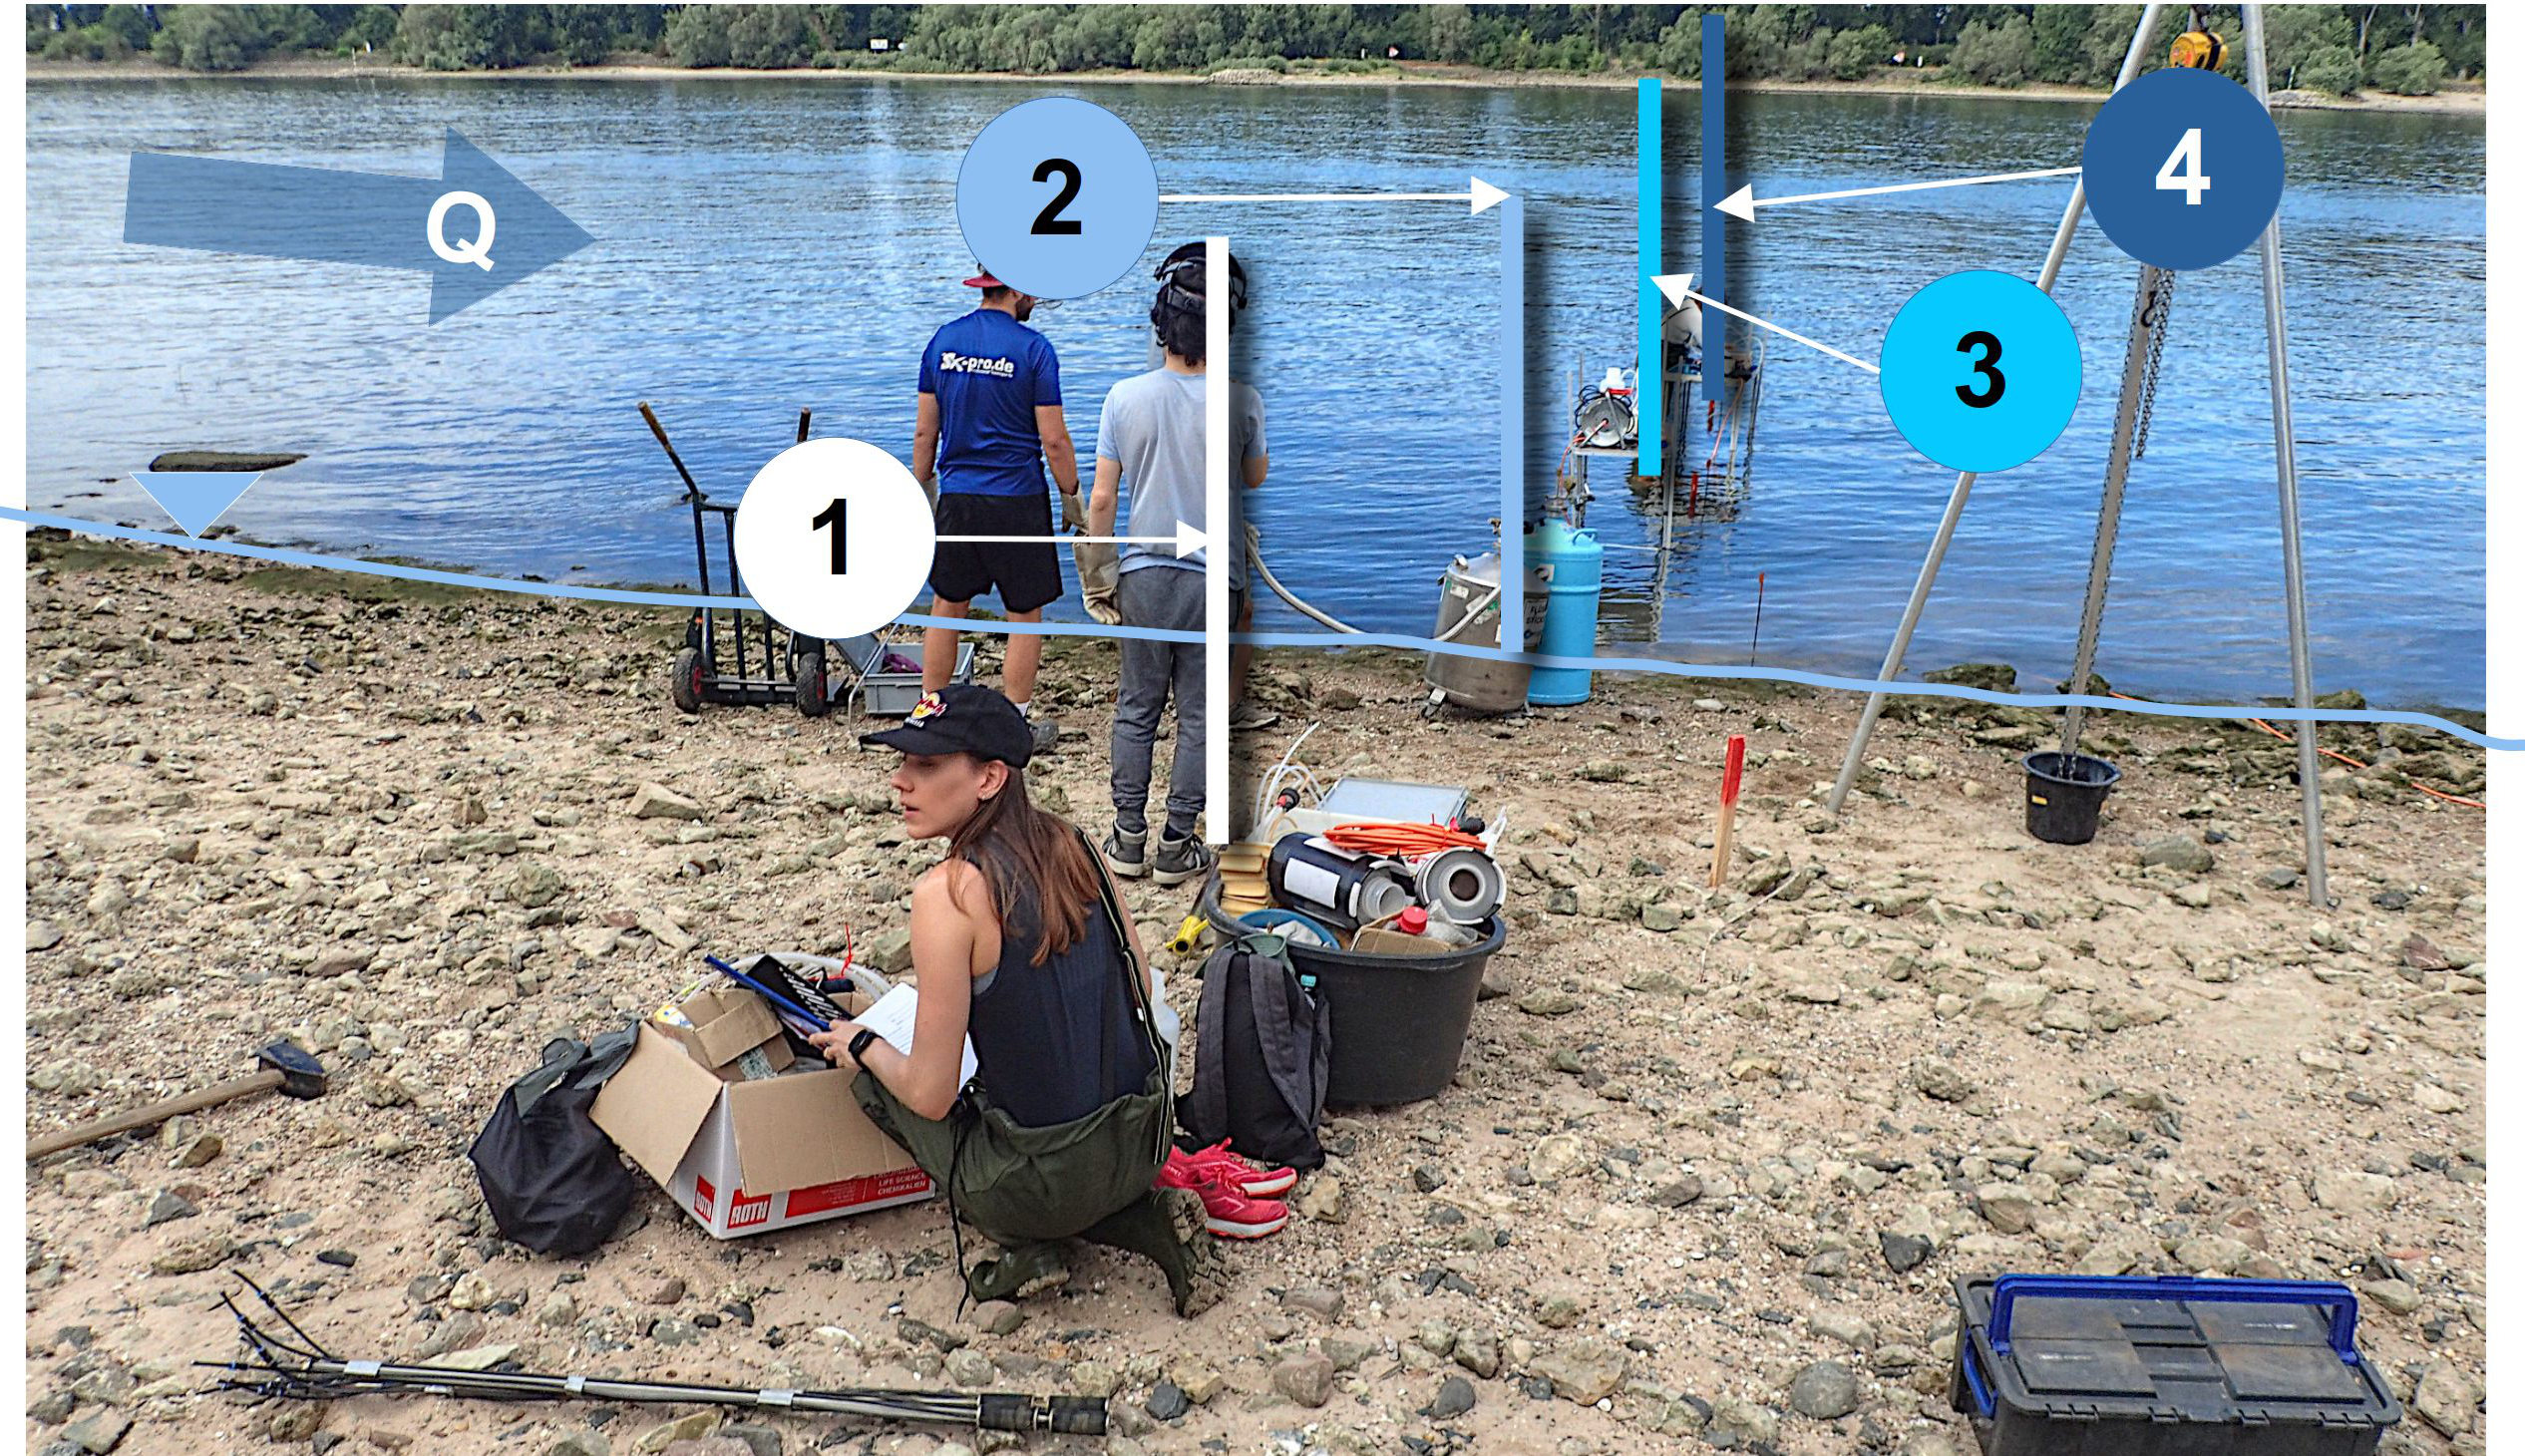
\includegraphics[width=0.88\paperwidth]{multipac-rhine}};
		\end{scope}}
	\end{tikzpicture}
\end{frame}



\begin{frame}{\secname\vspace{0.1cm}\\\textcolor{anthrazit!80!white}{\subsecname}}
	\begin{tikzpicture}
		\clip (0,0) rectangle (\paperwidth,\paperheight);
		\onslide<1->{
			\begin{scope}
				\node[anchor=south west, xshift=0.0\paperwidth, yshift=0.31\paperheight] {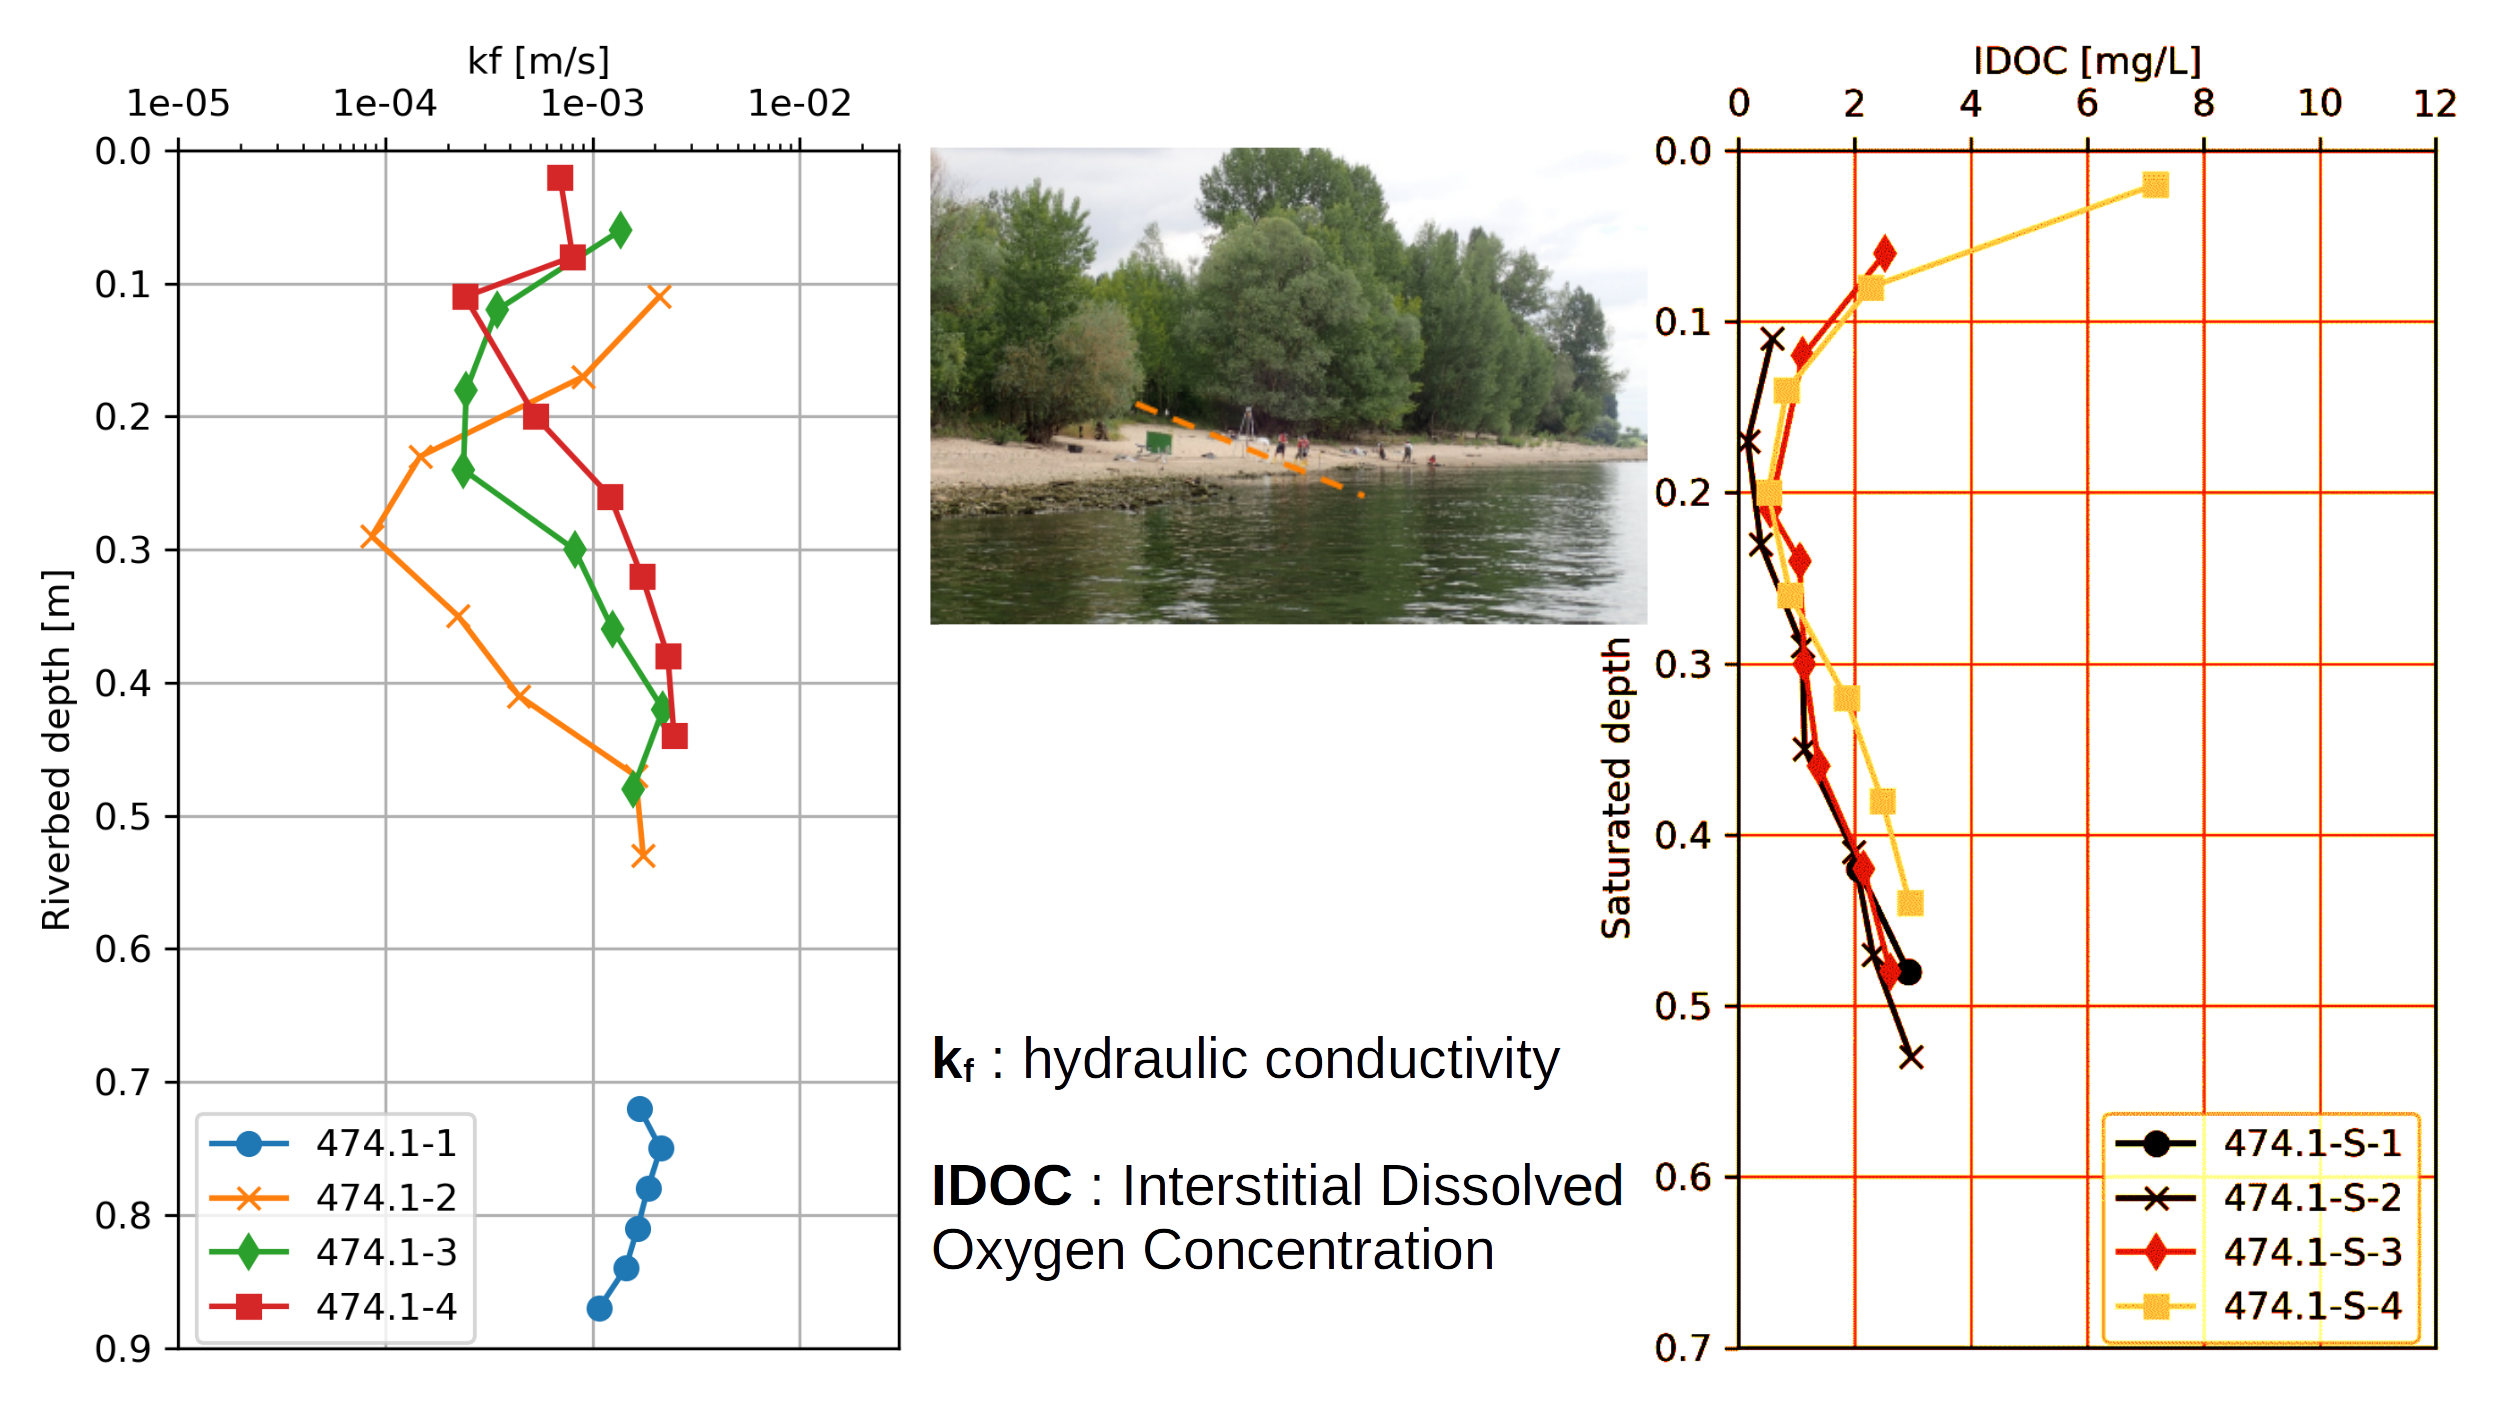
\includegraphics[width=0.9\paperwidth]{rhine-profiles-full}};
		\end{scope}}
	\end{tikzpicture}
\end{frame}


\begin{frame}{\secname\vspace{0.1cm}\\\textcolor{anthrazit!80!white}{\subsecname}}
	\begin{tikzpicture}
		\clip (0,0) rectangle (\paperwidth,\paperheight);
		\onslide<1->{
			\begin{scope}
				\node[anchor=south west, xshift=0.0\paperwidth, yshift=0.31\paperheight] {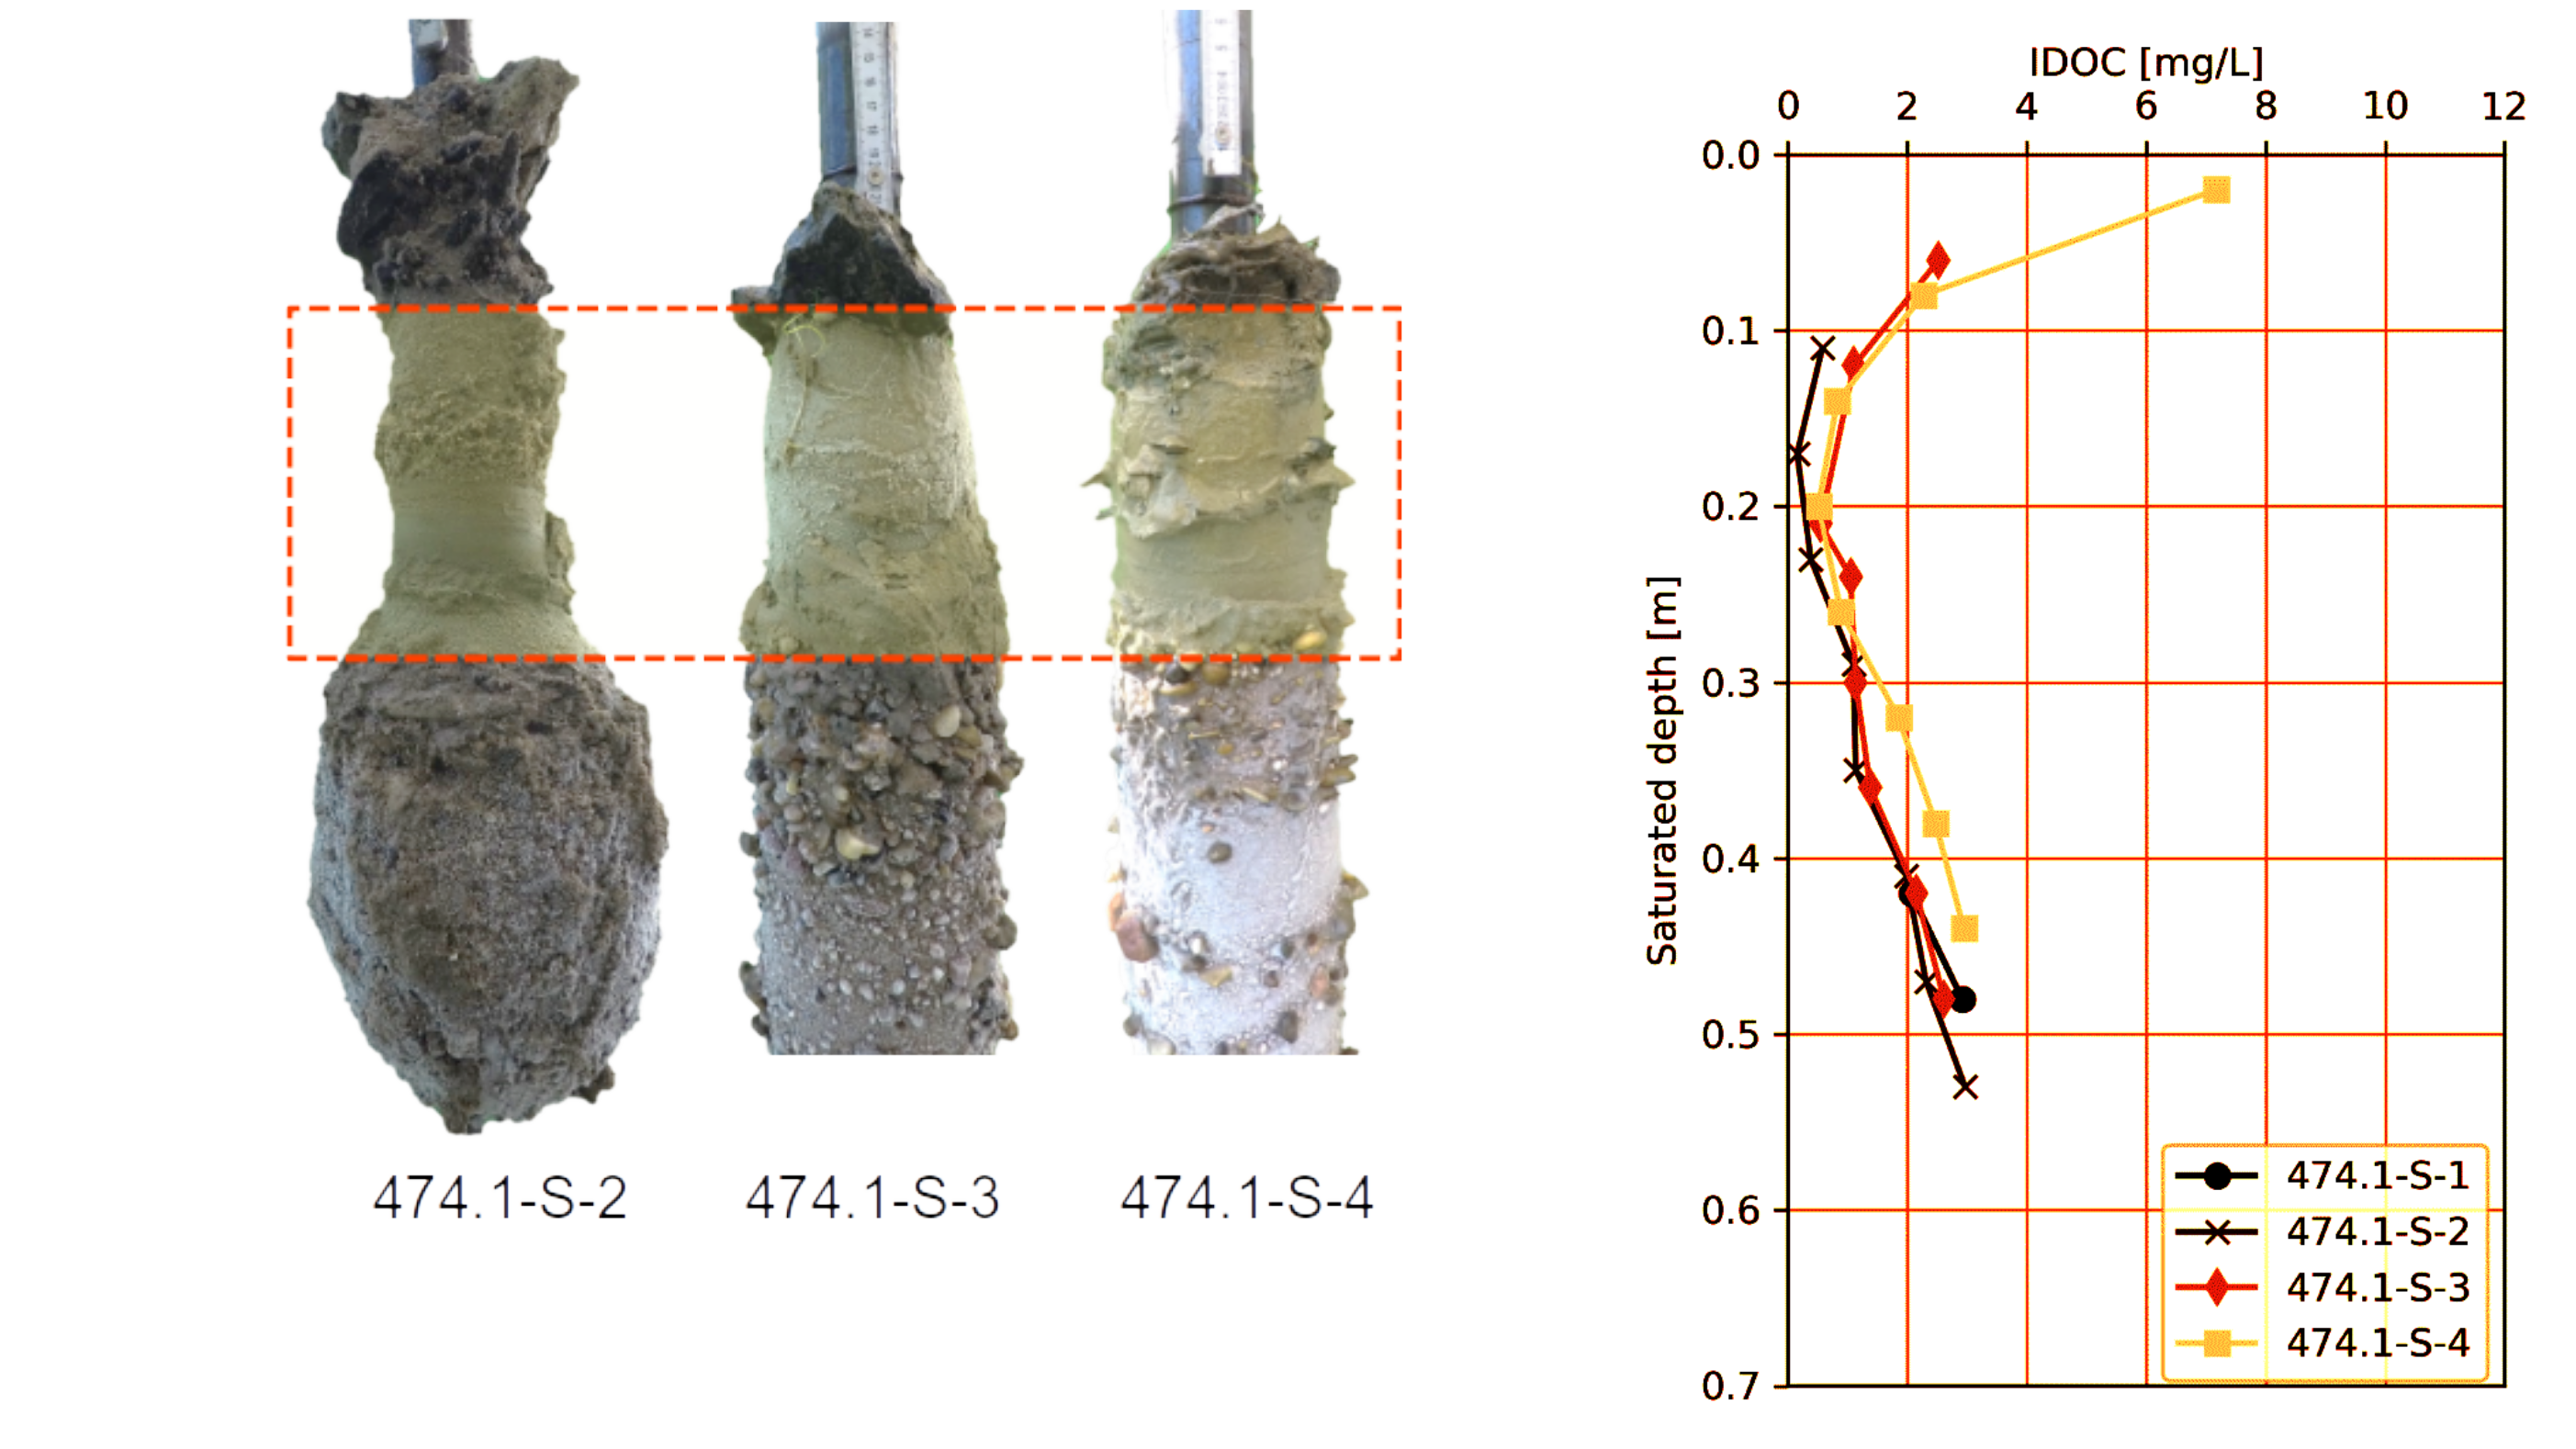
\includegraphics[width=0.9\paperwidth]{rhine-profiles-analysis}};
		\end{scope}}
	\end{tikzpicture}
\end{frame}


\begin{frame}{\secname\vspace{0.1cm}\\\textcolor{anthrazit!80!white}{\subsecname}}
	\begin{tikzpicture}
		\clip (0,0) rectangle (\paperwidth,\paperheight);
		\onslide<1->{
		\begin{scope}
				\node[anchor=south west, xshift=0.0\paperwidth, yshift=0.31\paperheight] {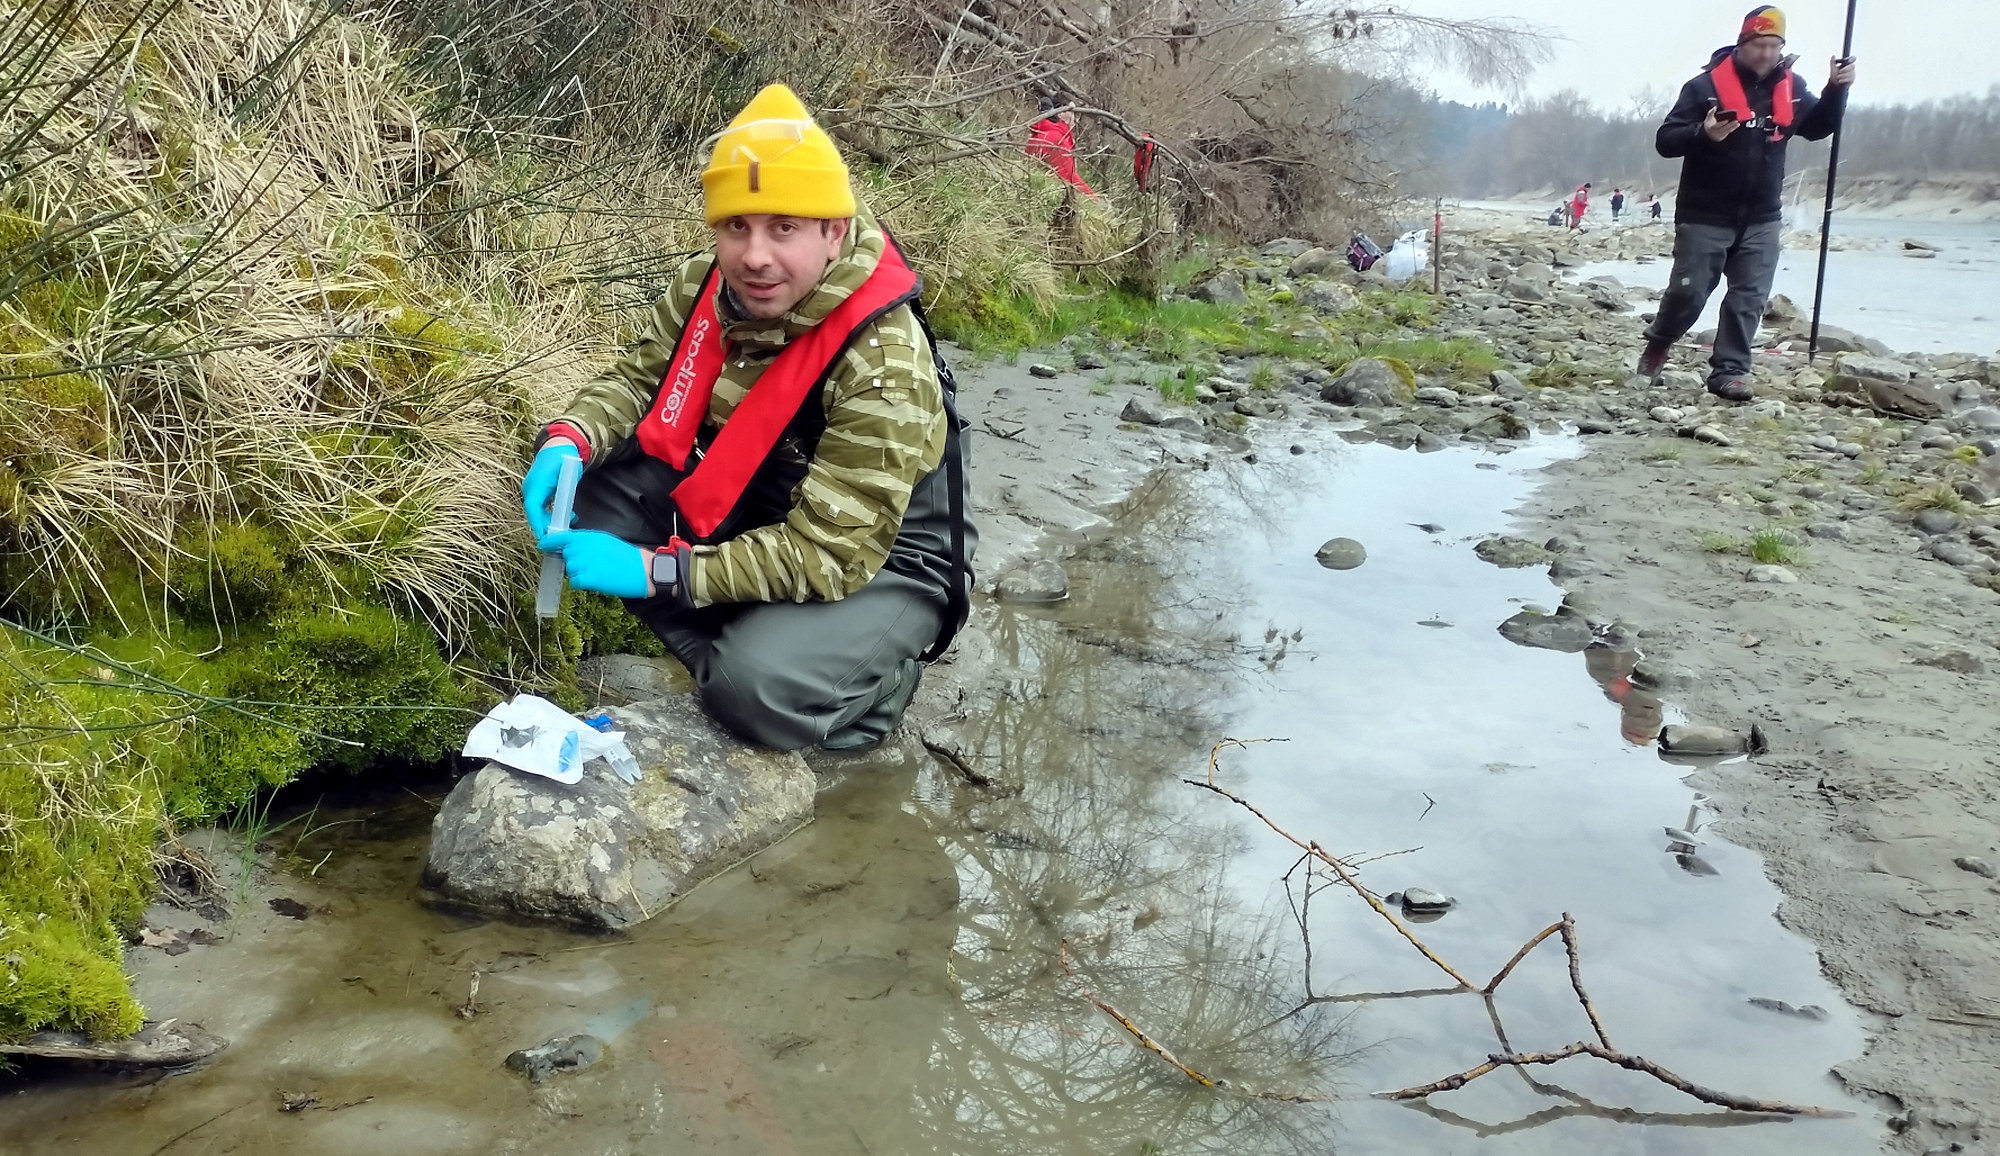
\includegraphics[width=0.88\paperwidth]{inn-new-campaign}};
		\end{scope}
		\begin{scope}
			\node[anchor=south west, xshift=0.0\paperwidth, yshift=0.31\paperheight] {
\includegraphics[width=0.88\paperwidth]{inn-new-campaign-overlay}};
		\end{scope}}
	\end{tikzpicture}
\end{frame}

\section{Wrap-up {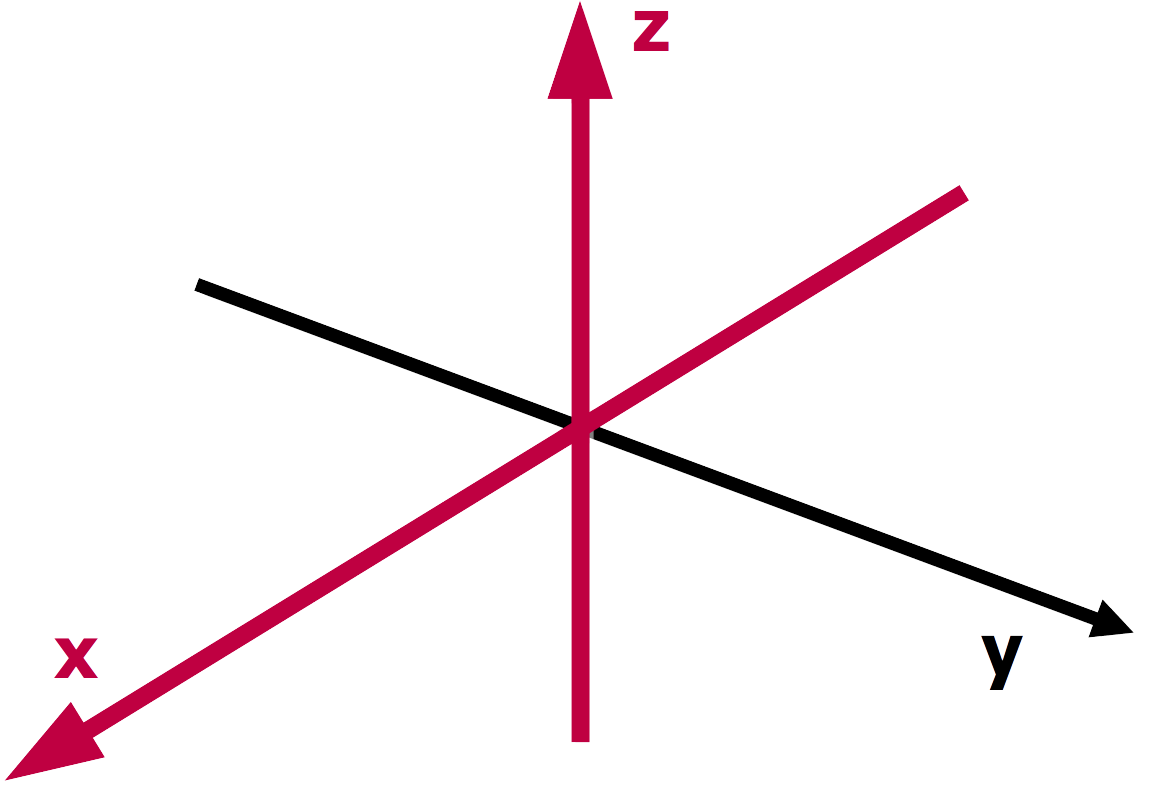
\includegraphics[height=15pt]{connectivity-xz-small}}}

{
\usebackgroundtemplate{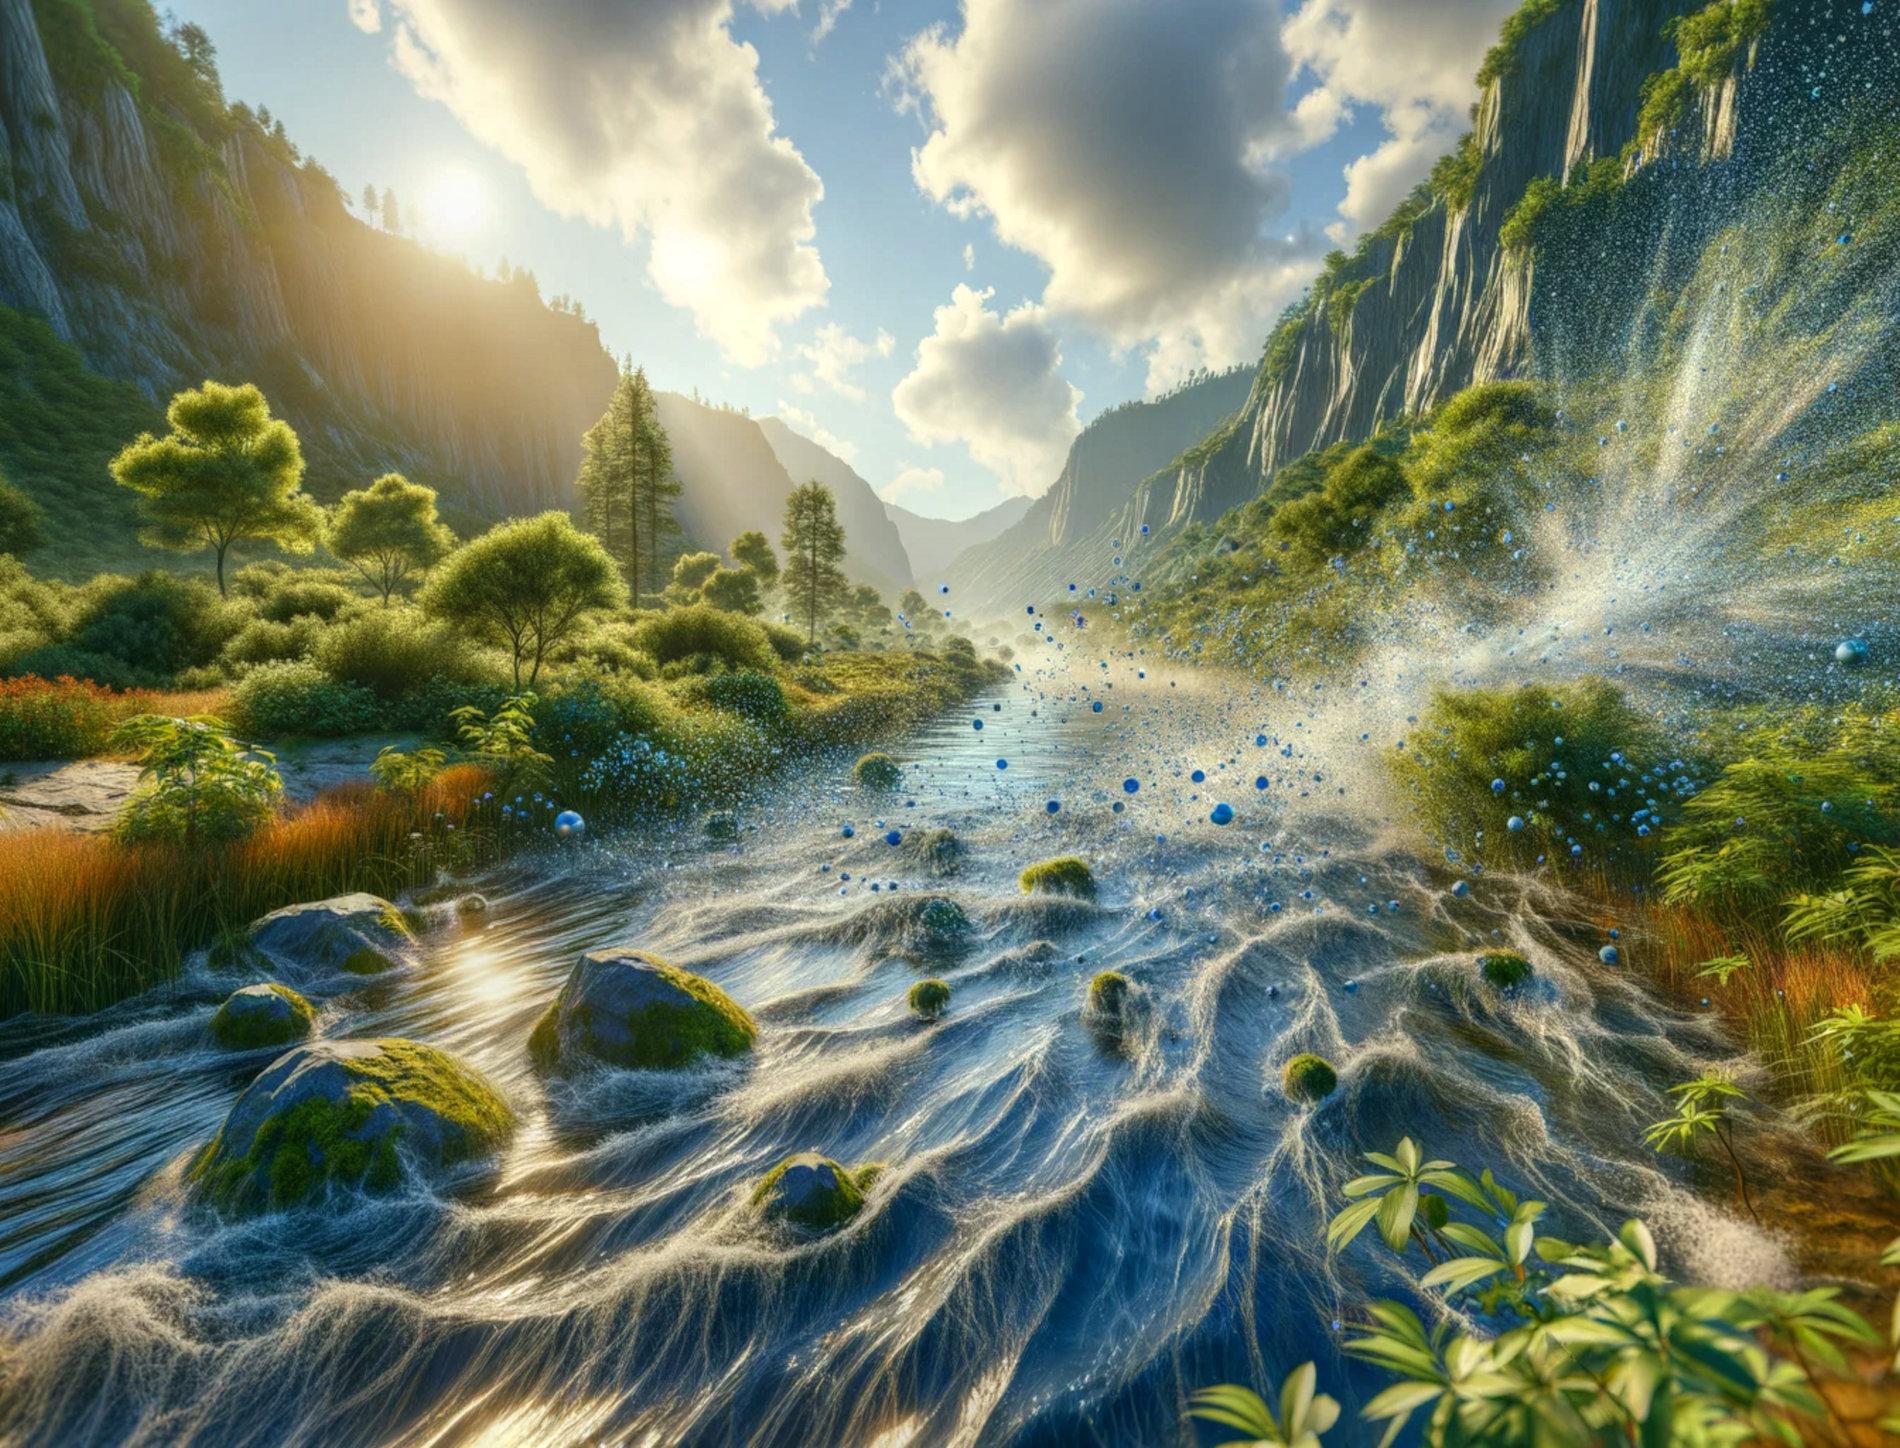
\includegraphics[width=\paperwidth]{final-background43.jpg}}%
\begin{frame}[plain]{}{\secname}
	\vspace{2.cm}
		\begin{tcolorbox}[colbacktitle=hellblau!80!black, colback=hellblau!10!white, fonttitle=\bfseries, standard jigsaw,colframe=blue_light, bottom=0mm, middle=0mm, boxsep=0.2mm, opacityframe=0.5, opacityfill=0.65, opacitybacktitle=0.75, title filled, title={\faGraduationCap\ Conclusions}, size=fbox]
			\vspace{0.25cm}
			\begin{itemize}			
				\item[\faChainBroken] Dams block primarily coarse sediment \& let pass very fine sediment\\
				$\rightarrow$ Downstream of dams: coarse sediment-hungry rivers only get fine sediment\\
				$\rightarrow$ Vertical disconnection (riverbed clogging) \& lateral disconnection \vspace{0.1cm}
				\item[\faLightbulbO] Numerical modeling provides predictive guidance for local actions, but calibration is challenging
				\item[\faLightbulbO] Local actions: improved sediment continuity in mountain rivers \& large wood placement
			\end{itemize}
			\vspace{0.1cm}
			\movie[externalviewer]{
\includegraphics[width=0.6\textwidth,keepaspectratio]{videos/blank-wide.png}}{videos/ue-fishpass-clip.mp4}
		\end{tcolorbox}
		\smallskip
\end{frame}
}



%%%%%%%%%%%%%%%%%%%%%%%%%%%%%%%%% final slide %%%%%%%%%%%%%%%%%%%%%%%%%%%%%%%%%%
% Two options: white and blue bg
%\thankyou{Thank you for your attention}{theme/logos/hyinfo.jpg}
\thankyou{Thank you}{Dr. sc. (PhD) Sebastian Schwindt}{sebastian.schwindt@iws.uni-stuttgart.de\\{\tiny https://www.iws.uni-stuttgart.de}}{+49 (0)711 685 64 789}{theme/logos/iws-logo.png}
	
\end{document}
